\documentclass[11pt]{article}

\usepackage[utf8]{inputenc}

\usepackage{mathpazo}
\usepackage{amssymb,amsthm}
\usepackage[fleqn]{amsmath}
\usepackage{bigints}
\usepackage[svgnames]{xcolor}
\usepackage{graphicx}
%\usepackage{animate}
\usepackage{media9}
\usepackage{manfnt}
\usepackage{textcomp}
\usepackage{hyperref}
\usepackage[breakable,theorems,skins]{tcolorbox}

\graphicspath{{asy/}}

%lengths
\unitlength 1cm
\textheight 22cm
\textwidth 17cm
\oddsidemargin -0.5cm
\evensidemargin -0.5cm
\topmargin -1.5cm
\topskip 0cm
\headheight 0.5cm
\headsep 1cm
\marginparwidth 1.2cm
\newlength\doubleind
\addtolength{\doubleind}{\leftmargini}
\addtolength{\doubleind}{\leftmarginii}

%MathNumbering
\makeatletter
\@addtoreset{equation}{section}
\renewcommand{\theequation}{\thesection.\@arabic\c@equation}
\newcommand\Nopagebreak{\@nobreaktrue\nopagebreak}
%\renewcommand{\theequation}{\@arabic\c@equation}
\makeatother

\newcommand\boldinline[1]{\paragraph{#1}}
\newcommand\boldsubsection[1]{\subsection*{#1}}
\newcommand\boldsubsubsection[1]{\subsubsection*{#1}}

\def\exstart{\hangindent\leftmargini\textup{1.}\hspace{\labelsep}}


%Theorems
\tcbset{
	defstyle/.style={enhanced, top=3pt, bottom=3pt, colframe=black, coltitle=black, arc=5pt, boxrule=1.5pt, left*=0pt, right*=0pt, theorem style=plain, terminator sign={.\ \ \ }, fonttitle=\bfseries\upshape, fontupper=\upshape, colback=blue!8!white, grow sidewards by=8pt, drop fuzzy shadow},
	exstyle/.style={enhanced, breakable, beforeafter skip balanced=10pt, coltitle=black, theorem style=plain, terminator sign={.\ \ \ }, fonttitle=\bfseries\upshape, fontupper=\upshape, blanker, borderline west={4pt}{-8pt}{orange!75!white}},
	thmstyle/.style={enhanced, top=3pt, bottom=3pt, colframe=black, coltitle=black, arc=5pt, boxrule=1.5pt,left*=0pt, right*=0pt, theorem style=plain, terminator sign={.\ \ \ }, fonttitle=\bfseries\upshape, fontupper=\slshape, colback=green!12!white, grow sidewards by=8pt, drop fuzzy shadow},
	exercisestyle/.style={enhanced, breakable, beforeafter skip balanced=10pt, coltitle=black, theorem style=plain, terminator sign={.\ \ \ }, fonttitle=\bfseries\upshape, fontupper=\upshape, blanker, borderline west={4pt}{-8pt}{purple!75!white}, title={Exercises\ \ \ }},
	proofstyle/.style={enhanced, breakable, beforeafter skip balanced=10pt, blanker, borderline west={4pt}{-8pt}{green!50!white}},
	asidestyle/.style={enhanced, breakable, beforeafter skip balanced=10pt, blanker, borderline west={4pt}{-8pt}{black!50!white}},
	exercisestyle2/.style={enhanced, breakable, beforeafter skip balanced=10pt, coltitle=black, theorem style=plain, terminator sign={.\ \ \ }, fonttitle=\bfseries\upshape, fontupper=\upshape, blanker, borderline west={4pt}{-8pt}{purple!75!white}, title={Exercises\ \thesubsection.\ \ \ }},
	exercisestyle4/.style={enhanced, breakable, beforeafter skip balanced=10pt, coltitle=black, theorem style=plain, terminator sign={.\ \ \ }, fonttitle=\bfseries\upshape, fontupper=\upshape, blanker, borderline west={4pt}{-8pt}{purple!75!white}, title={Exercises\ \thesection.\ \ \ }},
	exercisestyle3/.style={enhanced, breakable, beforeafter skip balanced=10pt, coltitle=black, theorem style=plain, terminator sign={.\ \ \ }, fonttitle=\bfseries\upshape, fontupper=\upshape, blanker, borderline west={4pt}{-8pt}{purple!75!white}, title={Exercise\quad}},
	}

\tcolorboxenvironment{proof}{breakable,proofstyle}


\newenvironment{proofpic}{%\topsep\relax
  \trivlist
  \item[\hskip\labelsep
        \itshape
    Proof.]\ignorespaces
}{\endtrivlist}


\newtcbtheorem[number within=section]{defn}{Definition}{defstyle}{defn}
\newtcbtheorem[use counter from=defn]{example}{Example}{exstyle}{ex}
\newtcbtheorem[use counter from=defn]{examples}{Examples}{exstyle}{ex}
\newtcbtheorem[use counter from=defn]{thm}{Theorem}{thmstyle}{thm}
\newtcbtheorem[use counter from=defn]{lemm}{Lemma}{thmstyle}{lemm}
\newtcbtheorem[use counter from=defn]{cor}{Corollary}{thmstyle}{cor}
\newtcbtheorem[use counter from=defn]{axiom}{Axiom}{defstyle}{axiom}
\newtcbtheorem[use counter from=defn]{axioms}{Axioms}{defstyle}{axioms}
\newtcbtheorem[use counter from=defn]{conj}{Conjecture}{thmstyle}{conj}

\newtcolorbox{aside}{asidestyle}
\newtcolorbox{exercises*}{exercisestyle}
\newtcolorbox{exercises}{exercisestyle2}
\newtcolorbox{exercisessec}{exercisestyle4}
\newtcolorbox{exercise}{exercisestyle3}
                      
\newenvironment{enumeratea}{
	\begin{enumerate}
	  \renewcommand{\labelenumi}{(\alph{enumi})}}
	{\end{enumerate}}

%lengths/commands
\def\lstsp{\hspace{\labelsep}}
\renewcommand{\qedsymbol}{\rule[-8pt]{0.5em}{0.5em}}
\def\marks#1{\hfill{\scriptsize{(#1)}}\par}
\def\dmarks#1{\tag*{\scriptsize{(#1)}}}
\def\prelistskip{\vspace*{-6pt}}
\def\preinitdisp{\setlength{\abovedisplayskip}{-15pt}}
\def\postinitdisp{\setlength{\abovedisplayskip}{12pt plus 3pt minus 9pt}}
\def\ang#1{#1\text{°}}
\def\st{\textsuperscript{st}}
\def\nd{\textsuperscript{nd}}
\def\rd{\textsuperscript{rd}}
\def\th{\textsuperscript{th}}
\def\AM{\,{a.m.}}
\def\PM{\,{p.m.}}
\def\BC{{\,\textsc{bc}}}
\def\AD{{\textsc{ad}\,}}

%mathrm
\def\I{\mathrm{I}}
\def\rL{\mathrm{L}}
\def\rU{\mathrm{U}}
\newcommand{\rO}{\mathrm{O}}
\newcommand{\rM}{\mathrm{M}}
\newcommand{\rS}{\mathrm{S}}
\newcommand{\rT}{\mathrm{T}}
\newcommand{\rSO}{\mathrm{SO}}
\newcommand{\rSL}{\mathrm{SL}}
\newcommand{\rSp}{\mathrm{Sp}}
\newcommand{\rGL}{\mathrm{GL}}
\newcommand{\rSU}{\mathrm{SU}}

%bbb
\def\C{\mathbb{C}}
\def\E{\mathbb{E}}
\def\F{\mathbb{F}}
\def\II{\mathbb{I}}
\def\K{\mathbb{K}}
\def\N{\mathbb{N}}
\def\Q{\mathbb{Q}}
\def\pr{\mathbb{P}}
\def\R{\mathbb{R}}
\def\Z{\mathbb{Z}}

%bold/linalg
\def\V#1{\mathbf{#1}}
\def\va{{\V a}}
\def\vb{{\V b}}
\def\vc{{\V c}}
\def\vd{{\V d}}
\def\ve{{\V e}}
\def\vf{{\V f}}
\def\vi{{\V i}}
\def\vj{{\V j}}
\def\vk{{\V k}}
\def\vn{{\V n}}
\def\vp{{\V p}}
\def\vq{{\V q}}
\def\vr{{\V r}}
\def\vs{{\V s}}
\def\vt{{\V t}}
\def\vu{{\V u}}
\def\vv{{\V v}}
\def\vw{{\V w}}
\def\vx{{\V x}}
\def\vy{{\V y}}
\def\vz{{\V z}}
\def\vB{{\V B}}
\def\vE{{\V E}}
\def\vF{{\V F}}
\def\vG{{\V G}}
\def\vN{{\V N}}
\def\vR{{\V R}}
\def\vT{{\V T}}

\def\ip#1{\left\langle #1\right\rangle}
\def\nm#1{\left| #1\right|}
\def\Nm#1{\nm{\nm{#1}}}
\def\lst#1#2{{#1}_1,\ldots,{#1}_{#2}}
\def\vect#1#2{\lst{\V{#1}}{#2}}
\def\lincom#1#2#3{{#1}_1\V{#2}_1+\cdots+{#1}_{#3}\V{#2}_{#3}}
\def\lincomsc#1#2#3{{#1}_1{#2}_1+\cdots+{#1}_{#3}{#2}_{#3}}
\def\proj{\operatorname{proj}}
\def\cl#1{\overline{#1}}
\def\hcf{\operatorname{hcf}}
\def\leg#1#2{\left(\frac{#1}{#2}\right)}
\def\lcm{\operatorname{lcm}}
\def\dom{\operatorname{dom}}
\def\Rank{\operatorname{rank}}
\def\Null{\operatorname{null}}
\def\quotient#1#2{{}^{\textstyle {#1}}\!\big/_{\textstyle \!{#2}}}
\def\spmod{\negthickspace\negthickspace\mod}
\def\Cov{\operatorname{Cov}}
\def\deg{\operatorname{deg}}
\def\ddeg{\operatorname{deg}}
\def\Arg{\operatorname{Arg}}

\def\twovec#1#2{\begin{pmatrix}#1\\#2\end{pmatrix}}
\def\stwovec#1#2{\left(\begin{smallmatrix}#1\\#2\end{smallmatrix}\right)}
\def\threevec#1#2#3{\begin{pmatrix}#1\\#2\\#3\end{pmatrix}}
\def\sthreevec#1#2#3{\left(\begin{smallmatrix}#1\\#2\\#3\end{smallmatrix}\right)}
\def\fourvec#1#2#3#4{\begin{pmatrix}#1\\#2\\#3\\#4\end{pmatrix}}
\def\sfourvec#1#2#3#4{\left(\begin{smallmatrix}#1\\#2\\#3\\#4\end{smallmatrix}\right)}
\newenvironment{smatrix}{\left(\begin{smallmatrix}}{\end{smallmatrix}\right)}

\def\lin#1{\overleftrightarrow{#1}}
\def\ray#1{\overrightarrow{#1}}
\def\rayv#1{\overrightarrow{\underline{#1}}}

%caligraphic
\def\cL{\mathcal{L}}
\def\cP{\mathcal{P}}
\def\cA{\mathcal{A}}
\def\cU{\mathcal{U}}
\def\cC{\mathcal{C}}
\def\cS{\mathcal{S}}
\def\cN{\mathcal{N}}
\def\cB{\mathcal{B}}
\def\cR{\mathcal{R}}
\def\cE{\mathcal{E}}


%gothic
\def\fc{\mathfrak{c}}
\def\fg{\mathfrak{c}}
\def\fo{\mathfrak{o}}
\def\fso{\mathfrak{so}}
\def\fsl{\mathfrak{sl}}

%shortcuts
\def\vphi{\varphi}
\def\vep{\varepsilon}

%calculus
\def\D{\mathrm{d}}
\def\dint{\displaystyle\int}
\def\at#1#2{\left.#1\right|_{#2}}
\newcommand{\diff}[2][]{\frac{\D #1}{\D #2}}
\newcommand{\diffat}[3][]{\left.\diff[#1]{#2}\right|_{#3}}
\newcommand{\partials}[2][]{\frac{\partial #1}{\partial #2}}
\newcommand{\partialsat}[3][]{\left.\partials[#1]{#2}\right|_{#3}}
\newcommand{\jacobian}[2]{\frac{\partial(#1)}{\partial(#2)}}
\newcommand{\jacthree}[6]{\begin{vmatrix}
				#1_#4&#1_#5&#1_#6\\
				#2_#4&#2_#5&#2_#6\\
				#3_#4&#3_#5&#3_#6
				\end{vmatrix}}
				
\def\df{{\D f}}
\def\dg{{\D g}}
\def\dr{{\D r}}
\def\ds{{\D s}}
\def\dt{{\D t}}
\def\du{{\D u}}
\def\dv{{\D v}}
\def\dw{{\D w}}
\def\dx{{\D x}}
\def\dy{{\D y}}
\def\dz{{\D z}}
\def\dA{{\D A}}
\def\dS{{\D S}}
\def\dV{{\D V}}
\def\dvn{\D{\V n}}
\def\dvr{\D{\V r}}
\def\dvx{\D{\V x}}
\def\dvS{\D{\V S}}
\def\dth{{\D\theta}}

%operators
\def\laplace#1{\cL\left\{#1\right\}}
\def\ad{\operatorname{ad}}
\def\tr{\operatorname{tr}}
\def\orb{\mathrm{orb}}
\let\divsymbol\div
%\def\div{\operatorname{div}}
\def\Div{\operatorname{div}}
\def\grad{\operatorname{grad}}
\def\curl{\operatorname{curl}}
\def\Hess{\operatorname{Hess}}
\def\Span{\operatorname{Span}}
\def\image{\operatorname{Im}}
\def\id{\operatorname{id}}
\DeclareMathOperator{\Stab}{Stab}
\DeclareMathOperator{\Fix}{Fix}
\DeclareMathOperator{\stab}{stab}
\DeclareMathOperator{\Aut}{Aut}
\DeclareMathOperator{\End}{End}
\DeclareMathOperator{\Int}{Int}
\DeclareMathOperator{\Inn}{Inn}
\def\Var{\operatorname{Var}}
\def\sgn{\mathrm{sgn}}
\def\diag{\operatorname{diag}}
\def\notimplies{\mathrel{{\ooalign{\hidewidth$\not\phantom{=}$\hidewidth\cr$\implies$}}}}
\usepackage{polynom}

\parindent0pt

\def\lin#1{\overleftrightarrow{#1}}
\def\ray#1{\overrightarrow{#1}}
\def\rayv#1{\overrightarrow{\underline{#1}}}
\def\arc#1{\overset{\raisebox{-3pt}[-5pt]{\smash{\rotatebox{90}{$)$}}}}{#1}}

\includeonly{
1axioms/axioms,
2euclid/euclid,
3analytic/analytic,
4hyper/hyper,
5fractals/fractals,
%TrigFormulas/trigformulas,
}

\allowdisplaybreaks

\begin{document}

\pagenumbering{arabic}
\thispagestyle{empty}
\graphicspath{{1axioms/asy/}}

\title{Math 161 - Notes}
\author{Neil Donaldson}
\date{Spring 2024}
\maketitle


\section{Geometry and the Axiomatic Method}\label{chap:axioms}

\subsection{The Early Origins of Geometry: Thales and Pythagoras}\label{sec:thales}


We begin with a condensed overview of geometric history. The word \emph{geometry} comes from the ancient Greek \emph{geo} (Earth), and \emph{metros} (measure). Measurement (of distance, area, height, angle) had obvious practical benefits with regard to construction, taxation, commerce and navigation. Astronomy provided a related cultural driver of ancient geometry.

\begin{description}
	\item[Ancient times] (pre-500\,\BC) Egypt, Mesopotamia, China, India: basic rules for measuring lengths, areas and volumes of simple shapes. Applications: surveying, tax collection, construction, religious practice, astronomy, navigation. Typically worked examples without general formulæ/abstraction.
	
	\item[Ancient Greece] (from c.\,600\,\BC) Philosophers such as Thales and Pythagoras began the process of \emph{abstraction.} General statements (theorems) formulated and proofs attempted. Concurrent development of early scientific reasoning.
	
	\item[Euclid of Alexandria] (c.\,300\,\BC) Collected and expanded earlier work, especially that of the Pytha\-goreans. His compendium the \emph{Elements} is one of the most important books in Western history and remained a standard school textbook in to the 1900's. The \emph{Elements} is an early exemplar of the axiomatic method at the heart of modern mathematics.
	
	\item[Later Greek Geometry] Archimedes' (c.\,270--212\,\BC) work on area and volume included techniques similar to those of modern calculus. %Apollonius studies conics (ellipses, parabolæ and hyperbolæ).
	Ptolemy (c.\,\AD\,100--170) writes the \emph{Almagest}, a treatise on astronomy which covers the foundations of trigonometry.
	
	\item[Post-Greek Geometry] During the European Dark Ages, geometric understanding was developed and enhanced by Indian and Islamic mathematicians who particularly developed trigonometry and algebra.
	
	\item[Analytic Geometry] In mid 1600's France, Descartes and Fermat melded algebra with geometry with the advent of co-ordinate systems (axes).
 	
	\item[Modern Development] Non-Euclidean geometries help provide the mathematical foundation for Einstein's relativity and the study of curvature. Following Klein (1872), modern geometry is highly dependent on group theory.
\end{description}



\boldinline{Thales of Miletus (c.\,624--546\,\BC)}

Thales was an olive trader from Miletus, a city-state on the west coast of modern Turkey. Through trading and travelling, he absorbed mathematical ideas from nearby cultures including Egypt and Mesopotamia. Here are five results partly attributable to Thales.
\begin{enumerate}\itemsep0pt
  \item A circle is bisected by a diameter.
  \item The base angles of an isosceles triangle are equal.
  \item The pairs of angles formed by two intersecting lines are equal.
  \item Two triangles are congruent if they have two angles and the included side equal.
  \item An angle inscribed in a semicircle is a right angle.
\end{enumerate}
The last is still known as \emph{Thales' Theorem.} Thales' arguments were not rigorous by modern standards. His real innovation was to state \emph{abstract, general principles}: \emph{any} circle is bisected by \emph{any} of its diameters. The Greek word $\theta\varepsilon\omega\rho\varepsilon\omega$ (\emph{theoreo}), from which we get \emph{theorem,} has several meanings: `to look at,' `speculate,' or `consider.' Thales' results were supposed to be clear just by looking at a picture.
\begin{center}
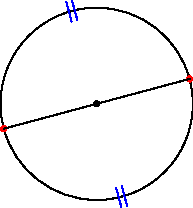
\includegraphics[scale=0.9]{thales-1}
\qquad\qquad
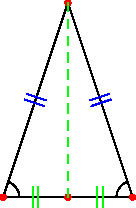
\includegraphics[scale=0.9]{thales-2}
\qquad\qquad
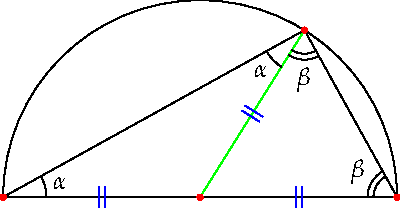
\includegraphics[scale=0.9]{thales-5}\label{thm:thales}
\end{center}
The pictures show Thales' Theorems 1, 2 and 5. Arguments for Theorems 1 and 2 could be as simple as `fold.' Theorem 5 follows from the observation that the \textcolor{Green}{radius} of the circle splits the large triangle into two isosceles triangles: Theorem 2 says that these have equal base angles (labelled), now check that $\alpha+\beta$ is half the angles in a triangle, namely a right-angle.


\boldinline{Pythagoras of Samos (570–-495\,\BC)}

Pythagoras grew up on Samos, an island in the Aegean Sea not far from Miletus. He also travelled widely, eventually settling in Croton, southern Italy, around 530\,\BC{} where he founded a philosophical school devoted to the study of number, music and geometry. It has been claimed that the Pythagoreans first classified the regular (Platonic) solids and developed the musical relationship between the length of a vibrating string and its pitch. While it is difficult to verify such assertions, the Pythagorean obsession with number and the `music of the universe' certainly inspired later mathematicians and philosophers---particularly Euclid, Plato and Aristotle---who believed they were refining and clarifying this earlier work.\smallbreak

Of course, Pythagoras is best known for the result that bears his name.

\begin{thm}{Pythagoras}{}
The square on the hypotenuse of a right triangle equals the sum of the squares on the remaining sides.
\end{thm}

Two important clarifications are needed for modern readers.
\begin{enumerate}\itemsep0pt
  \item By \emph{square,} the Greeks meant an honest square! There is no algebra, no numerical lengths, and the equation $a^2+b^2=c^2$ won't be seen for another 2000 years.
  \item The word \emph{equals} means \emph{equal area,} though without a numerical concept of such: the large square can be subdivided into pieces which may be rearranged to produce the two squares on the remaining sides.
\end{enumerate}

\goodbreak

The result suddenly seems less easy! The pictures below provide a simple visualization.

\begin{center}
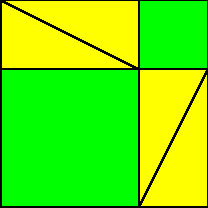
\includegraphics[width=0.3\linewidth]{pythag}
\qquad\qquad\qquad\qquad
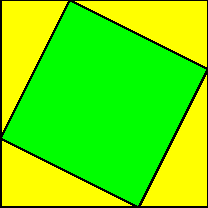
\includegraphics[width=0.3\linewidth]{pythag2}\medbreak
A simple proof of Pythagoras' Theorem
\end{center}
The problem with this `proof' is that it relies on \emph{subtracting} the areas of the four congruent triangles from a very large square, whereas the Greeks idea of area was essentially \emph{additive.} Book I of Euclid's \emph{Elements} seems to have been structured precisely to correct this and provide a rigorous constructive proof. Indeed it is possible (though very ugly!) to apply the 47 results leading up to and including his proof of Pythagoras, in such as way as to explicitly subdivide the hypotenuse square and rearrange it into the two smaller squares as required.\smallbreak


Much has been written about Pythagoras' Theorem, including many, many proofs.\footnote{Including a \href{https://www.maa.org/press/periodicals/convergence/mathematical-treasure-james-a-garfields-proof-of-the-pythagorean-theorem}{proof} by former US President James Garfield: would that current presidents were so learned\ldots} It is often claimed that Pythagoras himself first proved the result, but this is generally considered incorrect: the `proof' most often attributed to the Pythagoreans is based on contradictory ideas about numbers which were debunked by the time of Aristotle. Moreover, other cultures, particularly ancient China,\footnote{In China, Pythagoras' Theorem is known as the \emph{gou gu,} which refers to the two non-hypotenuse sides of the triangle.} are known to have used the result, at least in example form, several hundred years before Pythagoras. Regardless, an argument over attribution is fruitless without first agreeing on what constitutes a proof. This means that we need to spend some time considering Axiomatic Systems\ldots 


\begin{exercises}{}{}
\exstart Let the side-lengths of the above triangles be $a,b,c$. Can you rephrase the proof algebraically?
\begin{enumerate}\setcounter{enumi}{1}
	\item A theorem of Euclid states:
	\begin{quote}
	The square on the parts equals the sum of the squares on each part plus twice the rectangle on the parts
	\end{quote}
	By referencing the above picture, state Euclid's result using modern \emph{algebra.}\par
	(\emph{Hint: let $a$ and $b$ be the `parts'\ldots})
\end{enumerate}
\end{exercises}

\clearpage



\subsection{Axiomatic Systems}

%A primary motivation for Euclid's writing of the first book of the \emph{Elements} was to rigorously prove Pythagoras' Theorem. In so doing, he essentially invented the modern axiomatic method. %Before considering Euclid's approach, we describe the revolutionary structure Euclid followed, that of a \emph{deductive} or \emph{axiomatic system.}

Arguably the most revolutionary aspect of the \emph{Elements} was its axiomatic presentation.

\begin{defn}{}{}
An \emph{axiomatic system} comprises four types of object.\vspace{-5pt}
\begin{enumerate}\itemsep0pt
  \item \emph{Undefined terms}: Concepts accepted without definition/explanation. In basic geometry these would include \emph{line} and \emph{point.}
  \item \emph{Axioms}: Logical statements regarding the undefined terms which are accepted without proof.
  \item \emph{Defined terms}: Concepts defined in terms of 1 \& 2.
  \item \emph{Theorems}: Logical statements deduced from 1--3.
\end{enumerate}
\end{defn}


\begin{examples}{}{models}
Here are two systems viewed informally in this framework. In each case we provide only \emph{examples} of each type of object, not a full description of an axiomatic system.\vspace{-5pt}
\begin{description}\itemsep0pt
	\item[\normalfont\emph{Basic Geometry}]\begin{enumerate}\itemsep2pt
	  \item \emph{Line} and \emph{point.}
	  \item There exists a line joining any two given points.
	  \item A \emph{triangle} may be defined in using three non-collinear points. 
	  \item Thales' and Pythagoras' Theorems.
  \end{enumerate}
	\item[\normalfont\emph{Chess}]\begin{enumerate}\itemsep2pt
	  \item Pieces (as black/white objects) and the board.
	  \item Rules for how each piece moves.
	  \item Concepts such as \emph{check, stalemate} or \emph{en-passant.}
	  \item For example, \emph{Given a particular position, Black can win in 5 moves.}
  \end{enumerate}	
\end{description}
\end{examples}


A \emph{proof} is a logical argument demonstrating the truth of a theorem \emph{within an axiomatic system.} In practice, this is an ideal to which we aspire, and a proof is simply a convincing logical argument.



\begin{defn}{}{}
A \emph{model} is a choice/definition of the undefined terms such that all axioms are true.
\end{defn}

Models are often \emph{abstract} in that they depend on another axiomatic system. In a \emph{concrete} model, the undefined terms are real-world objects (where contradictions are impossible(!)). The big idea is this:
\begin{quote}
\emph{Any theorem proved within an axiomatic system is true in any model of that system.}
\end{quote}
Mathematical discoveries often hinge on the realization that seemingly separate discussions can be described in terms of models of a common axiomatic system.

\begin{example}{}{monoid}
\emph{Monoid}: \ If you've studied group theory, this should seem familiar.\vspace{-5pt}
\begin{quote}
	\begin{enumerate}%\itemsep0pt
	  \item A set $G$ and a binary operation $\ast$.
	  \item (A1)\lstsp Closure:\quad $\forall a,b\in G$, $a\ast b\in G$\\
  	\lstsp(A2)\lstsp Associativity:\quad $\forall a,b,c\in G$, \ $a\ast(b\ast c)=(a\ast b)\ast c$\\
  	\lstsp(A3)\lstsp Identity:\quad $\exists e\in G$ such that $\forall a\in G$, \ $a\ast e=e\ast a=a$
	  \item Concepts such as \emph{square} $a^2=a\ast a$, or \emph{commutativity} $a\ast b=b\ast a$.
	  \item For example, \emph{The identity is unique.}
	\end{enumerate}
\end{quote}
$(G,*)=(\Z,+)$ is an abstract model, where $e=0$. If you really want a concrete model, consider a single dot $\bullet$ on the page, equipped with the operation $\bullet *\bullet =\bullet$!
\end{example}

\goodbreak





\begin{defn}{}{}
Certain properties are desirable in an axiomatic system.
\begin{description}
	\item[\normalfont\emph{Consistency}] The system is free of contradictions.
	\item[\normalfont\emph{Independence}] An axiom is independent if it is not a theorem of the others. An axiomatic system is independent if all its axioms are. 
	\item[\normalfont\emph{Completeness}] Every valid proposition within the theory is \emph{decidable}; can be proved or disproved.
\end{description}
\end{defn}

We unpack these ideas slightly. By necessity, our descriptions are vague; many notions need to be clarified (e.g.\ what is meant by a \emph{valid proposition}) before these ideas can be made rigorous.
\begin{description}\itemsep0pt
	\item[\normalfont\emph{Consistency}] May be demonstrated by exhibiting a \emph{concrete model.} An \emph{abstract model} demonstrates \emph{relative consistency}, dependent on the consistency of the underlying system. An inconsistent system is essentially useless.
	\item[\normalfont\emph{Independence}] To demonstrate the independence of an axiom, exhibit two models; one in which all axioms are true, the other in which only the considered axiom is false. 
	\item[\normalfont\emph{Completeness}] This is very unlikely to hold for most useful axiomatic systems in mathematics, though \href{https://en.wikipedia.org/wiki/Complete_theory}{examples} do exist. To show incompleteness, an \emph{undecidable}\footnote{A famous example of an undecidable statement from standard set theory is the \emph{Continuum Hypothesis,} which states that there is no uncountable set with cardinality strictly smaller than that of the real numbers.} statement is required, which can be viewed as a new independent axiom of an enlarged system. 
	\end{description}


\begin{example*}{\ref{ex:monoid}, cont}{}
The axiomatic system for a monoid is:
\begin{description}\itemsep0pt
	\item[\normalfont\emph{Consistent}] We have a (concrete) model.
	\item[\normalfont\emph{Independent}] Consider three models:
	\begin{itemize}\itemsep0pt
	  \item $(\N,+)$ satisfies axioms A1 and A2 but not A3.
	  \item $(\{e,a,b\},*)$ defined by the following table satisfies A1 and A3 but not A2
	  \[\begin{array}{c||ccc}
	  *&e&a&b\\\hline\hline
	  e&e&a&b\\
	  a&a&e&a\\
	  b&b&b&a
	  \end{array} \qquad \text{e.g.}\quad a*(b*b)=a*a=e\neq a=a*b=(a*b)*b\]
	  \item $(\Z\setminus\{1\},+)$ satisfies axioms A2 and A3 but not A1.
	\end{itemize}
	\item[\normalfont\emph{Incomplete}] The proposition `\emph{A monoid contains at least two elements}' is undecidable \emph{just from the axioms.} For instance, $(\{0\},+)$ and $(\Z,+)$ are models with one/infinitely many elements.\smallbreak
	  We could also ask if all elements have an inverse. That this is undecidable is the same as saying that a new axiom is independent of A1, A2, A3.\smallbreak
	  \lstsp\lstsp\lstsp(A4) \ Inverse:\quad $\forall g\in G,\ \exists g^{-1}\in G$ such that $g\ast g^{-1}=g^{-1}\ast g=e$.\smallbreak
	The new system defined by the four axioms is also consistent and independent; this is the structure of a \emph{group.} Even this is incomplete however; consider a new axiom of commutativity\ldots
\end{description} 
\end{example*}

\goodbreak

\begin{example}{Bus Routes}{}
Here is a loosely defined axiomatic system. Discuss the questions with your classmates.
\begin{description}\itemsep0pt
	\item[\normalfont\emph{Undefined Terms}:] Route, Stop
	\item[\normalfont\emph{Axioms}:]\begin{description}
		\item[\normalfont (A1)] Each route is a list of stops in some order. These are the stops visited by the route.
		\item[\normalfont (A2)] Each route visits at least four distinct stops.
		\item[\normalfont (A3)] No route visits the same stop twice, except the first stop which is also the last stop.
		\item[\normalfont (A4)] There is a stop called downtown that is visited by each route.
		\item[\normalfont (A5)] Every stop other than downtown is visited by at most two routes.
	\end{description}
\end{description}

\begin{enumerate}
  \item Construct a model of this system with three routes. What is the fewest number of stops you can use?
  \item Your answer to 1 shows that this system is: complete, consistent, inconsistent, independent?
  \item Is the following a model for the Bus Routes system? If not, determine which axioms are satisfied by the model and which are not?
  \begin{quote}\def\arraystretch{1.2}
  \begin{tabular}{@{}ll}
    \emph{Stops}:&Downtown, \ Walmart, \ Albertsons, \ Main St., \ CVS, \ Trader Joe's, \ Zoo\\
  	\emph{Route 1}:&Downtown, \ Walmart, \ Main St., \ CVS, \ Zoo, \ Downtown\\
  	\emph{Route 2}:&Main St., \ CVS, \ Zoo, \ Albertsons, \ Downtown, \ Main St.\\
  	\emph{Route 3}:&Walmart, \ Main St., \ Downtown, \ Albertsons, \ Main St., \ Walmart
  \end{tabular}
  \end{quote}
	\item Show that A3 is independent of the other axioms.
	\item Demonstrate that `\emph{There are exactly three routes}' is not a theorem in this system by finding a model in which it is not true.
\end{enumerate}
\end{example}

\vfil

We are only scratching the surface of axiomatics here. If you really want to dive down the rabbit hole, consider taking a class in formal logic or model theory. As an example of the ideas involved, we finish with two results proved in 1931 by the German logician Kurt Gödel.

\begin{thm}{Gödel's incompleteness theorems}{} 
\begin{enumerate}
  \item Any consistent system containing the natural numbers is incomplete.
  \item The consistency of such a system cannot be proved within the system itself.
\end{enumerate}
\end{thm}

Gödel's first theorem tells us that there is no \emph{ultimate} consistent complete axiomatic system. Perhaps this is reassuring; there will always be undecidable statements, so mathematics will never be finished! However, the undecidable statements cooked up by Gödel are analogues of the famous \emph{liar paradox} (`This sentence is false'), so the profundity of this is a matter of debate.\smallbreak
Gödel's second theorem fleshes out the difficulty in proving the consistency of an axiomatic system. If a system is sufficiently complex to describe the natural numbers, its consistency can at best be proved relative to some other axiomatic system; while an inconsistent system might be essentially useless, good luck showing that what you have really is consistent!
\goodbreak

\begin{exercises}{}{}
\exstart Between two players are placed several piles of coins. On each turn a player takes as many coins as they want from \emph{one} pile, as long as they take at least one coin. The player who takes the last coin wins.

\begin{enumerate}\setcounter{enumi}{1}
  \item[]If there are two piles where one pile has more coins than the other, prove that the first player can always win the game.
  \item Consider a system where children in a classroom choose different flavors of ice cream. Suppose we have the following axioms:
  \begin{quote}
  \begin{itemize}%[align=left]
  	\item[(A1)] There are exactly five flavors of ice cream: vanilla, chocolate, strawberry, cookie dough, and bubble gum.
  	\item[(A2)] Given any two distinct flavors, there is exactly one child who likes these.
  	\item[(A3)] Every child likes exactly two flavors of ice cream.
  \end{itemize}
  \end{quote}
  \begin{enumerate}%[align=left]
    \item How many children are in the classroom? Prove your assertion.
    \item Prove that any pair of children likes at most one common flavor.
    \item Prove that for each flavor, there are exactly four children who like that flavor.
	\end{enumerate}
	
% 	\item Here is a very simple and informal list of axioms; terms such as \emph{class, students, pass, grade, etc.,} might be undefined, though this isn't critical for our purposes.
% 	\begin{itemize}%\setlength\itemsep{0pt}
%   	\item[](B1) \ There are exactly 18 students in a class.
% 		\item[](B2) \ Sixteen students pass the class, and two students do not.
% 		\item[](B3) \ Arturo and Bella both get the same grade.
% 	\end{itemize}
% 	\begin{enumerate}
% 	  \item Discuss whether this system is consistent, independent and/or incomplete.
% 	  \item Suppose we add a fourth axiom:\\
% 	  (B4) \ All students have the same name.\\
% 	  What happens? 
% 	\end{enumerate}	
% 	

% \begin{description}
%   \item[]\emph{Consistent}\lstsp With a little effort even a concrete model is possible; just grab 18 students, change names if necessary and assign some grades!
%   \item[]\emph{Non-independent}\lstsp B1 is a theorem of B3.
%   \item[]\emph{Incomplete}\lstsp Do any other students obtain the same grade as Arturo? This is unanswerable from the axioms.
% \end{description}


	\item Consider an axiomatic system that consists of elements in a set $S$ and a set $P$ of pairings of elements $(a,b)$ that satisfy the following axioms:
  \begin{quote}
  \begin{itemize}%[align=left]
  	\item[(A1)] If $(a,b)$ is in $P$, then $(b,a)$ is not in $P$.
  	\item[(A2)] If $(a,b)$ is in $P$ and $(b,c)$ is in $P$, then $(a,c)$ is in $P$.
  \end{itemize}
  \end{quote}
  \begin{enumerate}%[align=left]
    \item Let $S=\{1,2,3,4\}$ and $P=\{(1,2),(2,3),(1,3)\}$. Is this a model for the axiomatic system? Why/why not?
		\item Let $S$ be the set of real numbers and let $P$ consist of all pairs $(x,y)$ where $x<y$. Is this a model for the system? Explain.
		\item Use the results of (a) and (b) to argue that the axiomatic system is incomplete. I.e., think of another independent axiom that could be added to the axioms A1 and A2 for which $S$ and $P$ in part (a) is a model, but for which $S$ and $P$ from part (b) is not a model.
	\end{enumerate}
	
	\item The undefined terms of an axiomatic system are `brewery' and `beer'. Here are some axioms.
  \begin{quote}
	\begin{itemize}%[align=left]
  	\item[(A1)] Every brewery is a non-empty collection of \emph{at least} two beers (every brewery brews at least two beers!).
  	\item[(A2)] Any two distinct breweries have at most one beer in common.
  	\item[(A3)] Every beer belongs to exactly three breweries.
  	\item[(A4)] There exist exactly six breweries.
	\end{itemize}
  \end{quote}
  \begin{enumerate}%[align=left]
    \item Prove the following theorems.
    \begin{enumerate}
      \item There are exactly four beers.
      \item There are exactly two beers in each brewery.
      \item For each brewery, there is exactly one other brewery which has no beers in common.
  	\end{enumerate}
  	\item Prove that the axioms are independent.\par
  	(\emph{When negating A1, you should assume that a brewery is still a collection of beers, but that any such could contain none or one beer})
  \end{enumerate}
\end{enumerate}
\end{exercises}
\graphicspath{{2euclid/asy/},{2euclid/pics/}}

\section{Euclidean Geometry}\label{chap:euclid}

\subsection{Euclid's Postulates and Book I of the Elements}\label{sec:euclid}

Euclid's \emph{Elements} (c.\,300\,\BC) formed a core part of European and Arabic curricula until the mid 20\th{} century. Several examples are shown below.
\begin{center}
	\newlength{\heighttt}
	\setlength{\heighttt}{100pt}
	\begin{minipage}[b]{0.35\linewidth}
		\centering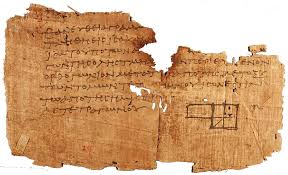
\includegraphics[height=\heighttt]{euclid1}\\
		Earliest Fragment c.\,\AD\,100
	\end{minipage}
	\begin{minipage}[b]{0.3\linewidth}
		\centering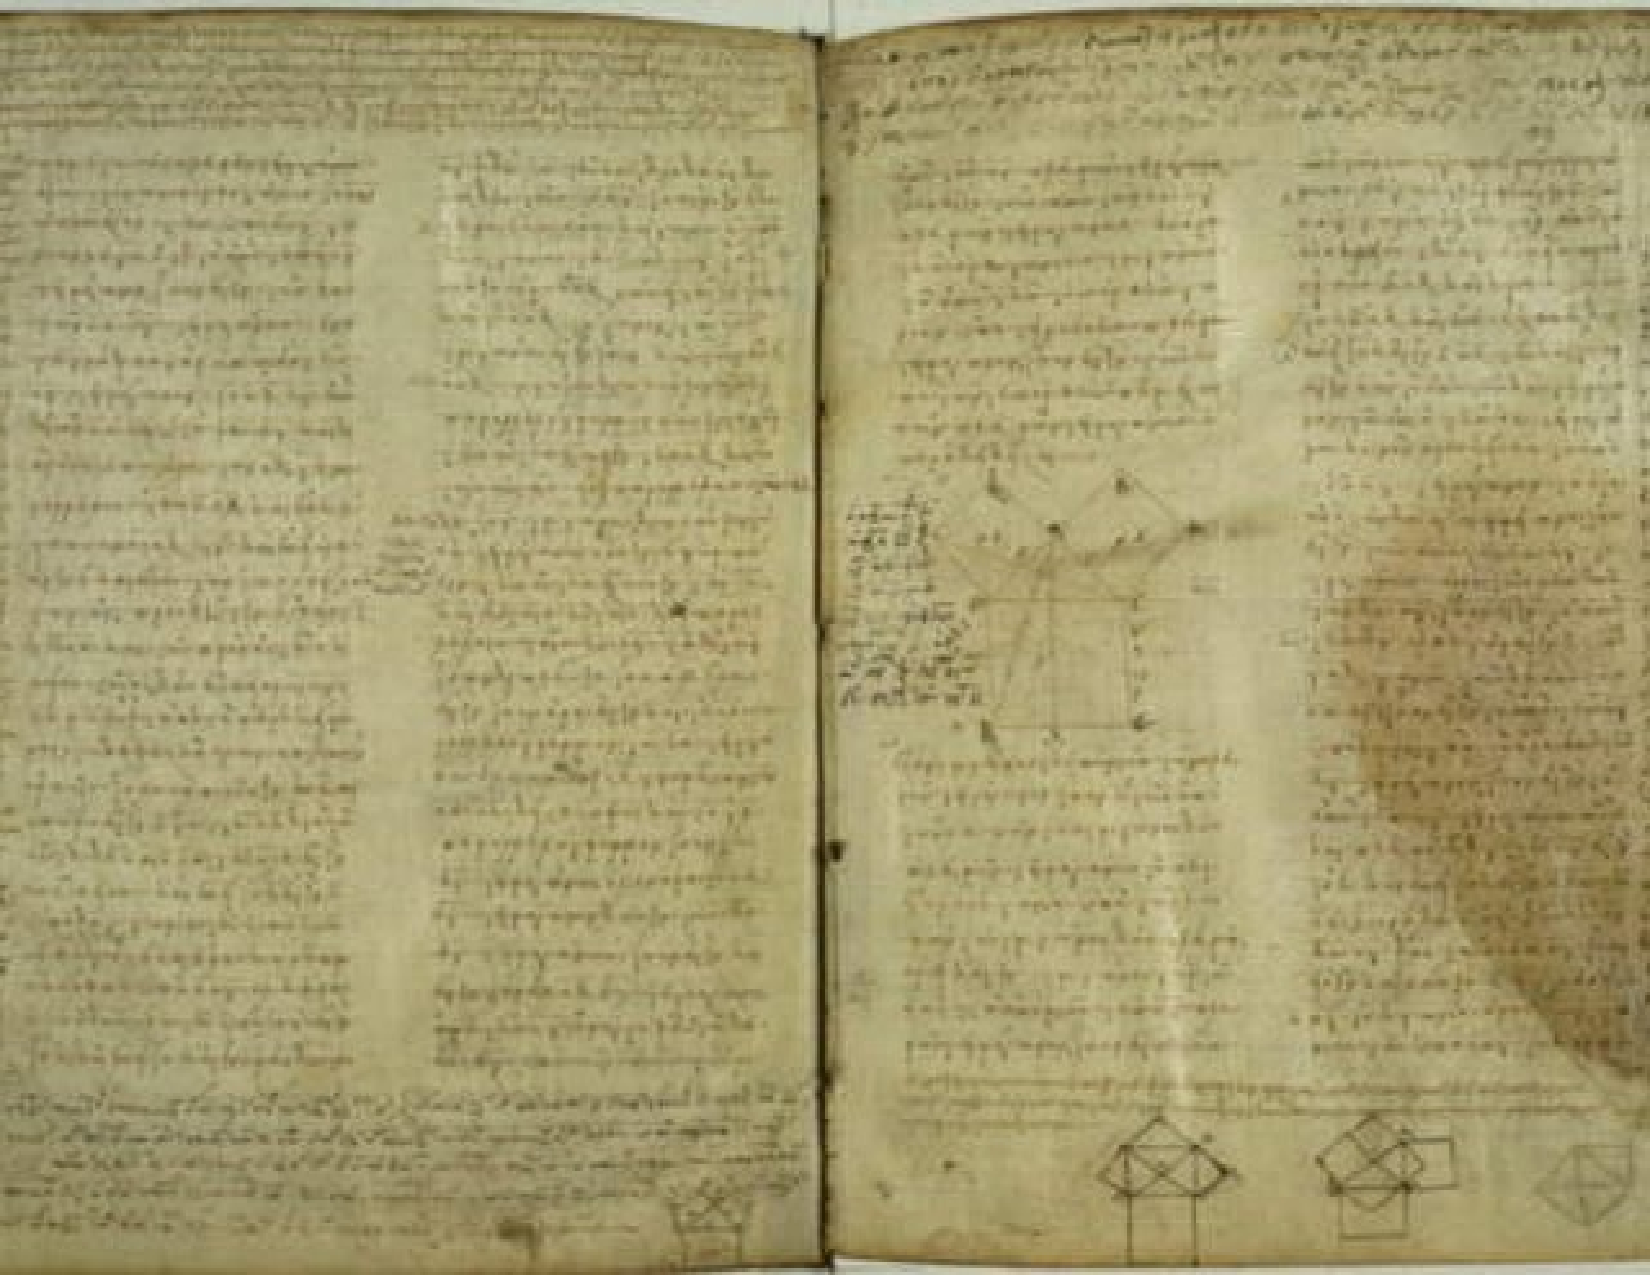
\includegraphics[height=\heighttt]{euclid2}\\
		Full copy, Vatican, 9\th\,C
	\end{minipage}
	\begin{minipage}[b]{0.33\linewidth}
		\centering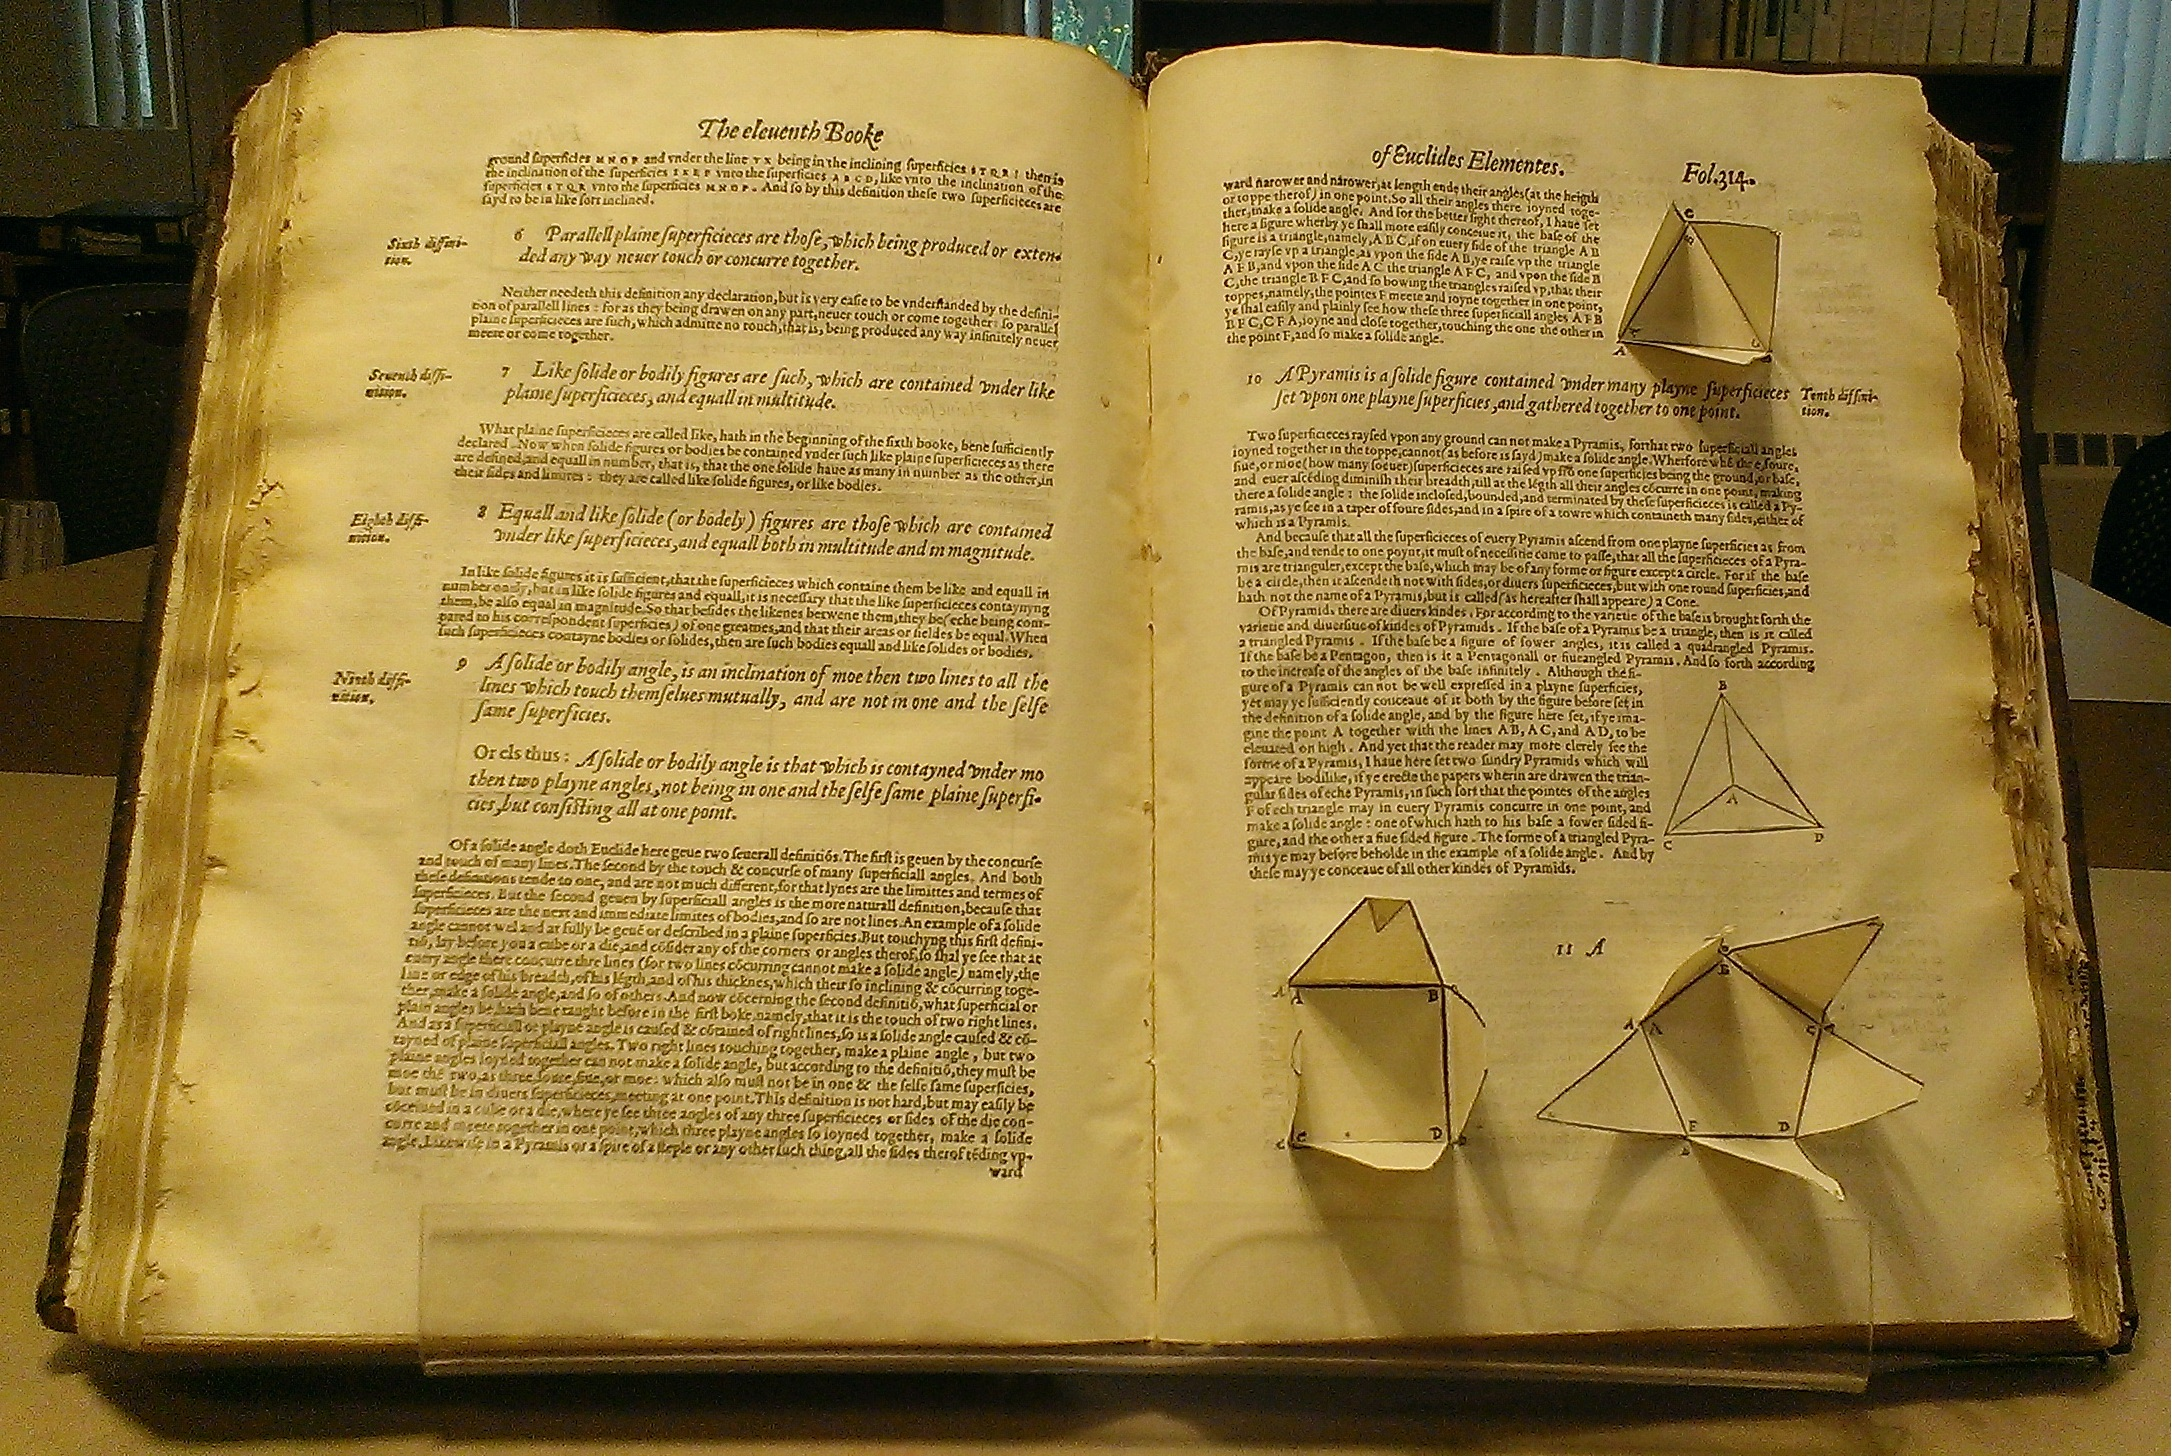
\includegraphics[height=\heighttt]{euclid3}\\
		Pop-up edition, 1500s
	\end{minipage}\\[5pt]
	\setlength{\heighttt}{135pt}
	\begin{minipage}[b]{0.44\linewidth}
		\centering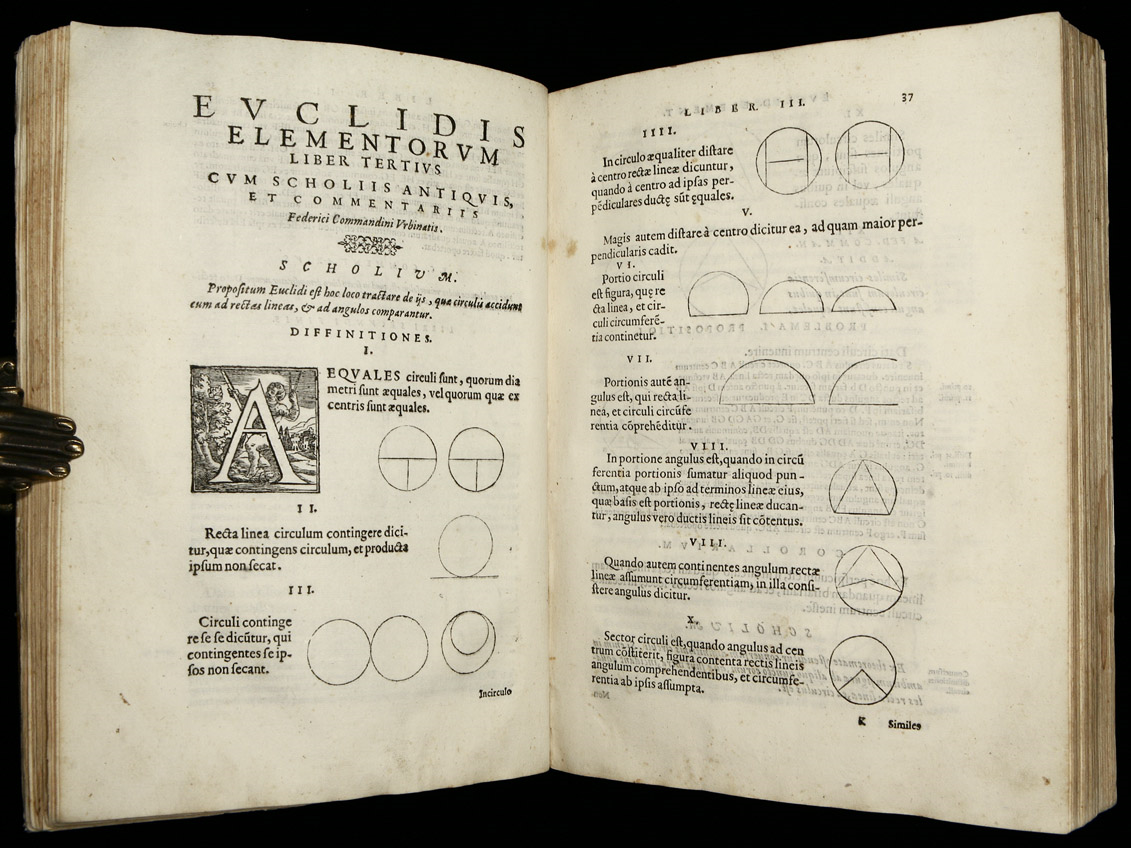
\includegraphics[height=\heighttt]{geo-09-euclid}\\
		Latin translation, 1572
	\end{minipage}
	\begin{minipage}[b]{0.3\linewidth}
		\centering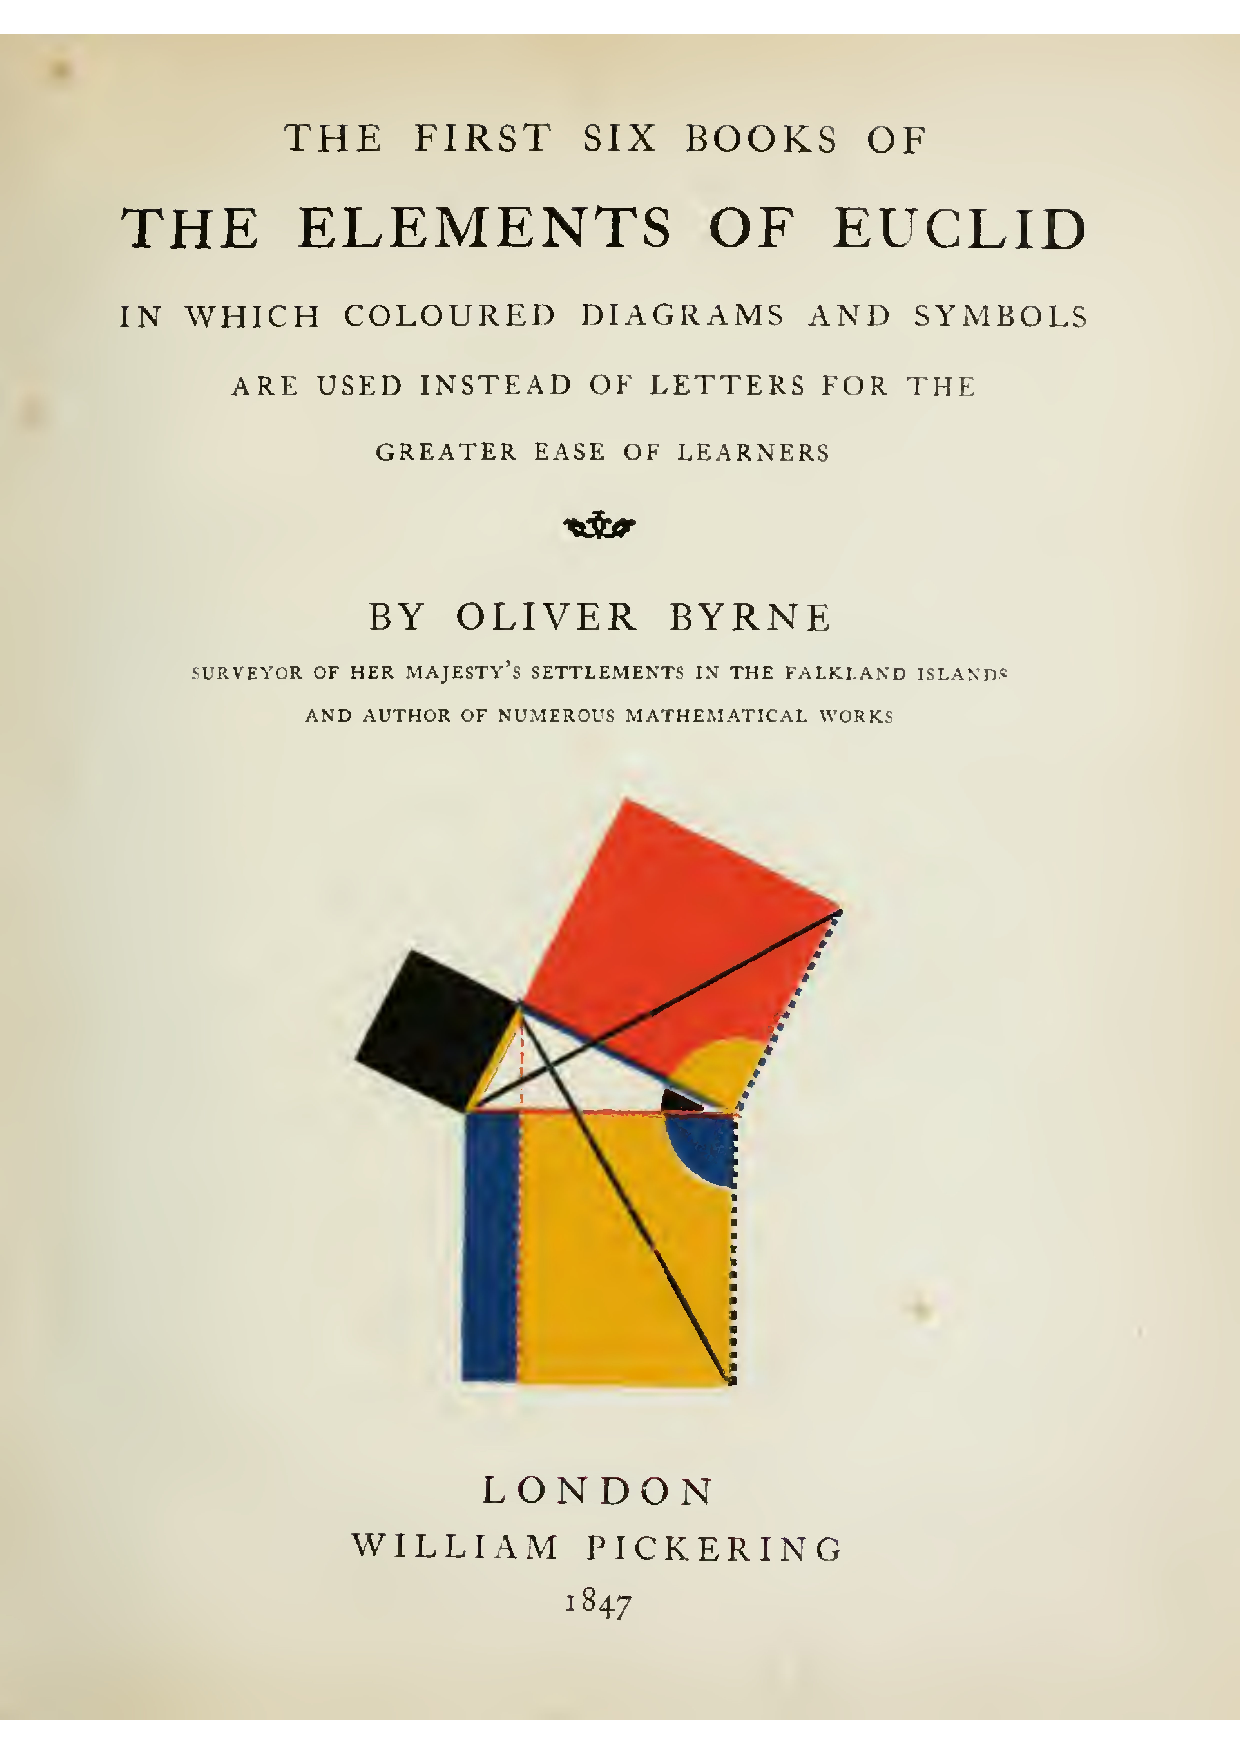
\includegraphics[height=\heighttt]{euclid5}\\
		Color edition, 1847
	\end{minipage}
	\begin{minipage}[b]{0.24\linewidth}
		\centering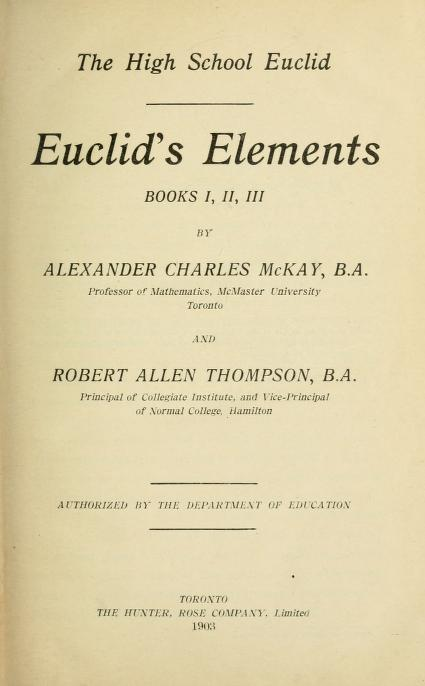
\includegraphics[height=\heighttt]{euclid4}\\
		Textbook, 1903
	\end{minipage}
\end{center}

Many of Euclid's arguments can be found \href{http://math.furman.edu/~jpoole/euclidselements/euclid.htm}{online}, and you can read Byrne's 1847 edition \href{http://math.uci.edu/~ndonalds/Elements-I-VI.pdf}{here}: the cover is Euclid's proof of Pythagoras'. We present an overview of Book I.

%to address some of the shortcomings in Euclid's original approach, it contains a more comprehensive list of definitions, has more axioms, and relabels propositions 4 and 5 as axioms (pages xviii--xxiii). 

\begin{description}\itemsep0pt
	\item[\normalfont\emph{Undefined Terms}] E.g., point, line, etc.\footnote{In fact Euclid attempted to define these: `A point is that which has no part,' and `A line has length but no breadth.'}
	\item[\normalfont\emph{Axioms/Postulates}]\negthickspace\!\footnote{In Euclid, an axiom is considered somewhat more general than a postulate. Here the postulates contain the \emph{geometry.}}\lstsp A1\lstsp If two objects equal a third, then the objects are equal\hfill ($=$ is transitive)\vspace{-5pt}
	\begin{itemize}
		\item[A2] If equals are added to equals, the results are equal\hfill ($a=c$ \& $b=d\implies a+b=c+d$)
		\item[A3] If equals are subtracted from equals, the results are equal
		\item[A4] Things that coincide are equal (in magnitude)
		\item[A5] The whole is greater than the part
		\item[P1] A pair of points may be joined to create a line
		\item[P2] A line may be extended
		\item[P3] Given a center and a radius, a circle may be drawn
		\item[P4] All right-angles are equal
		\item[P5] If a straight line crosses two others and the angles on one side sum to less than two right-angles then the two lines (when extended) meet on that side.
	\end{itemize}
\end{description}

\goodbreak

The first three postulates describe the intuitive \emph{ruler and compass constructions.} P4 allows Euclid to compare angles at different locations. P5 is usually known as the \emph{parallel postulate.}
\bigbreak

Euclid's system doesn't quite fit the modern standard. Some axioms are vague (what are `things'?) and we'll consider several more-serious shortcomings later. For now we clarify two issues and introduce some notation.
\begin{description}
	\item[\normalfont\emph{Segments}] To Euclid, a line had \emph{finite} extent; we call such a \emph{(line) segment}: the segment joining points $A,B$ is denoted $\cl{AB}$. In modern geometry, a \emph{line} extends as far as is permitted.
	\item[\normalfont\emph{Congruence}] Euclid uses \emph{equal} where modern mathematicians say \emph{congruent}. We'll express, say, congruent angles as $\angle ABC\cong\angle DEF$ rather than $\angle ABC=\angle DEF$.
\end{description}


\boldsubsubsection{Basic Theorems à la Euclid}

Theorems were typically presented as a \emph{problem}; Euclid first provides a construction (P1--P3) before proving that his construction solves the problem.

\begin{thm}{I.\,1}{euclid1-1}
	Problem: to construct an equilateral triangle on a given segment.
\end{thm}

The labelling I.\,1 indicates Book I, Theorem 1.

\begin{tcolorbox}[proofstyle, lower separated=false, sidebyside, sidebyside align=top seam, sidebyside gap=0pt, righthand width=0.35\linewidth]
	\emph{Proof.}\ \ Given a line segment $\cl{AB}$:\smallbreak
	By P3, construct circles centered at $A$ and $B$ with radius $\cl{AB}$.\smallbreak
	Call one of the intersection points $C$; by P1, construct $\cl{AC}$ and $\cl{BC}$.\smallbreak
	We claim that $\triangle ABC$ is equilateral.\medbreak
	Observe that $\cl{AB}$ and $\cl{AC}$ are radii of the circle centered at $A$, while $\cl{AB}$ and $\cl{BC}$ are radii of the circle centered at $B$. By Axiom A1, the three sides of $\triangle ABC$ are congruent.
	\tcblower
	\flushright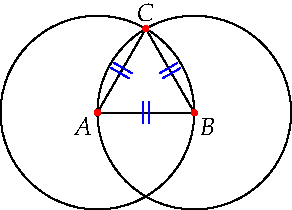
\includegraphics{euclid-I1}\hfil\qedsymbol
\end{tcolorbox}


Euclid proceeds to develop several well-known constructions and properties of triangles.
\begin{itemize}\itemsep0pt
  \item (I.\,4) Side-angle-side (SAS) congruence: if two triangles have two pairs of congruent sides and the angles between these are congruent, then the remaining sides and angles are congruent in pairs.
  \[
  	\begin{cases}
		  \cl{AB}\cong\cl{DE}\\
		  \angle ABC\cong\angle DEF\\
		  \cl{BC}\cong\cl{EF}
 	 	\end{cases}
  	\quad\implies
  	\begin{cases}
		  \cl{AC}\cong\cl{DF}\\
		  \angle BCA\cong\angle EFD\\
		  \angle CAB\cong\angle FDE
  	\end{cases}
  \]
  \item (I.\,5) An isosceles triangle has congruent base angles.
  \item (I.\,9) To bisect an angle.
  \item (I.\,10) To find the midpoint of a segment.
  \item (I.\,15) If two lines/segments cut one another, opposite angles are congruent.
\end{itemize}
Have a look at some of Euclid's arguments online. These are worth reading despite there being logical issues with Euclid's presentation. We'll revisit these results in the Exercises and next two sections. 

\goodbreak


\boldsubsubsection{Parallel Lines: Construction \& Existence}

\begin{defn}{}{parallel}
	Lines are \emph{parallel} if they do not intersect. Segments are parallel if no extensions of them intersect.
\end{defn}

In Euclid, a line is not parallel to itself. The next result is one of the most important in Euclidean geometry; it describes how to create a parallel line through a given point.


\begin{thm}[lower separated=false, sidebyside, sidebyside align=top seam, sidebyside gap=0pt, righthand width=0.37\linewidth]{I.\,16\ Exterior Angle Theorem}{extangle}
	If one side of a triangle is extended, then the exterior angle is larger than either of the opposite interior angles.\smallbreak
	In the picture, we have $\delta>\alpha$ and $\delta>\beta$.
	\tcblower
	\flushright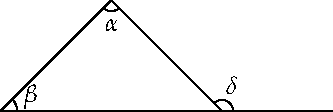
\includegraphics{euclid-I16}
\end{thm}

Euclid did not quantify angles numerically: $\delta>\alpha$ means that $\alpha$ is congruent to some angle \emph{inside} $\delta$.

\begin{proof}
	Construct the bisector $\cl{BM}$ of $\cl{AC}$ \ (I.\,10).\par
	\begin{minipage}[t]{0.64\linewidth}\vspace{-5pt}
		Extend $\cl{BM}$ to $E$ such that $\cl{BM}\cong\cl{ME}$ \  (I.\,2) and connect $\cl{CE}$ \  (P1).\smallbreak
		The opposite angles at $M$ are congruent \ (I.\,15).\smallbreak
		SAS (I.\,4) applied to $\triangle AMB$ and $\triangle CME$ says $\angle BAM\cong\angle EMC$, which is clearly smaller than the exterior angle at $C$.
	\end{minipage}
	\hfill
	\begin{minipage}[t]{0.35\linewidth}\vspace{-20pt}
		\flushright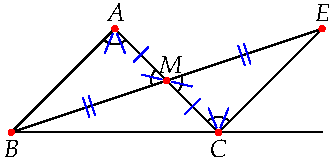
\includegraphics{euclid-I16p}
	\end{minipage}
	\smallbreak
	Bisect $\cl{BC}$ and repeat the argument to see that $\beta<\delta$.
\end{proof}

The proof in fact \emph{constructs} a parallel ($\cl{CE}$) to $\cl{AB}$ through $C$, as the next result shows.

\begin{thm}[lower separated=false, sidebyside, sidebyside align=top seam, sidebyside gap=0pt, righthand width=0.32\linewidth]{I.\,27}{}
	If a line falls on two other lines such that the alternate angles ($\alpha,\beta$) are congruent, then the two lines are parallel.
	\tcblower
	\flushright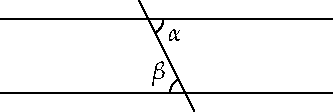
\includegraphics{euclid-I27}
\end{thm}

The \emph{alternate angles} in the exterior angle theorem are those at $A$ and $C$: $\cl{CE}$ really is parallel to $\cl{AB}$.

\begin{tcolorbox}[proofstyle,lower separated=false, sidebyside, sidebyside align=top seam, sidebyside gap=0pt, righthand width=0.37\linewidth]
	\emph{Proof.}\lstsp If the lines were not parallel, they would meet on one side. WLOG suppose they meet on the right side at $C$.\smallbreak
	The angle $\beta$ at $B$, being exterior to $\triangle ABC$, must be greater than the angle $\alpha$ at $A$ \ (I.\,16): contradiction.
	\tcblower
	\flushright
	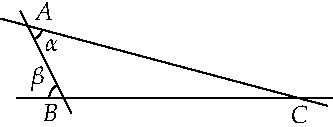
\includegraphics{euclid-I27p}\\[-12pt]\hfill\qedsymbol
\end{tcolorbox}

Euclid combines this with the vertical angles theorem (I.\,15) to finish the first half of Book I.

\begin{cor}[lower separated=false, sidebyside, sidebyside align=top seam, sidebyside gap=0pt, righthand width=0.32\linewidth]{I.\,28}{}
	If a line falling on two other lines makes congruent angles, then the two lines are parallel.
	\tcblower
	\flushright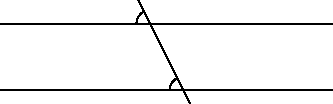
\includegraphics{euclid-I28}
\end{cor}


Thus far, Euclid uses only postulates P1--P4. In any model in which these hold:
\[
	\tcbhighmath{\text{Given a line $\ell$ and a point $C$ not on $\ell$, \textbf{there exists} a parallel to $\ell$ through $C$}}
\]
\goodbreak


\boldsubsubsection{Parallel Lines: Uniqueness, Angle-sums \& Playfair's Postulate}


Euclid finally invokes the parallel postulate to prove the converse of I.\,27, showing that the congruent alternate angle approach is the \emph{only} way to have parallel lines.

\begin{thm}{I.\,29}{}
	If a line falls on two parallel lines, then the alternate angles are congruent.
\end{thm}

\begin{tcolorbox}[proofstyle,lower separated=false, sidebyside, sidebyside align=top seam, sidebyside gap=0pt, righthand width=0.37\linewidth]
	\emph{Proof.}\ \ Given the picture, we must prove that $\alpha\cong\beta$.\smallbreak
	Suppose not and WLOG that $\alpha>\beta$.\smallbreak
	But then $\beta+\gamma<\alpha+\gamma$, which is a straight edge.\smallbreak
	By the parallel postulate, the lines $\ell,m$ meet on the left side of the picture, whence $\ell$ and $m$ are not parallel.
	\tcblower
	\flushright
	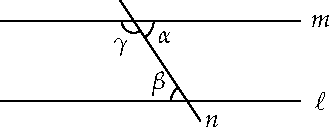
\includegraphics{euclid-I29}\\[-10pt]\qedsymbol
\end{tcolorbox}

The most well-known result about triangles is now in our grasp; the interior angles sum to a straight edge. Euclid words this slightly differently.

\begin{thm}{I.\,32}{}
	If one side of a triangle is extended, the exterior angle is congruent to the sum of the opposite interior angles.
\end{thm}

\begin{minipage}[t]{0.62\linewidth}\vspace{-4pt}
	\emph{This is not a numerical sum,} though for familiarity's sake we'll often write \ang{180} for a straight edge and \ang{90} for a right-angle.\par
	In the picture we've labelled angles as Greek letters for clarity. The result amounts to showing that $\widetilde\alpha+\widetilde\beta\cong\alpha+\beta$.
\end{minipage}
\hfill
\begin{minipage}[t]{0.37\linewidth}\vspace{-9pt}
	\flushright
	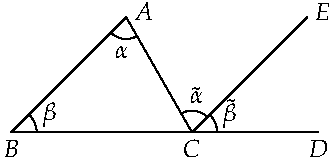
\includegraphics{euclid-I32}
\end{minipage}

\vspace{-20pt}

\begin{proof}
	Construct $\cl{CE}$ parallel to $\cl{BA}$ as in I.\,16, so that $\widetilde\alpha\cong\alpha$.\smallbreak
	$\cl{BD}$ falls on parallel lines $\cl{AB}$ and $\cl{CE}$, whence $\widetilde\beta\cong\beta$ (Corollary of I.\,29).\smallbreak
	Axiom A2 shows that $\angle ACD=\widetilde\alpha+\widetilde\beta\cong\alpha+\beta$.
\end{proof}


\medskip


The parallel postulate is stated in the negative (angles \emph{don't} sum to a straight edge, therefore lines are \emph{not} parallel). Though we cannot be sure, Euclid possibly chose this formulation in order to facilitate proofs by contradiction. Unfortunately the effect is to obscure the meaning of the parallel postulate. Here is a more modern interpretation.

\begin{axiom}[lower separated=false, sidebyside, sidebyside align=top seam, sidebyside gap=0pt, righthand width=0.37\linewidth]{Playfair's Postulate}{playfair}
	Given a line $\ell$ and a point $C$ not on $\ell$, \textbf{at most one} parallel line $m$ to $\ell$ passes through $C$.
	\tcblower
	\flushright
	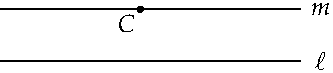
\includegraphics{euclid-playfair-defn}
\end{axiom}


\begin{minipage}[t]{0.62\linewidth}\vspace{0pt}
	Our discussion up to now shows that the parallel postulate implies Playfair.
	\begin{itemize}\itemsep0pt
	  \item Let $A,B\in\ell$ and construct the triangle $\triangle ABC$.
	  \item The exterior angle theorem constructs $E$ and thus a parallel $m$ to $\ell$ by I.\,27.
	  \item I.\,29 invokes the parallel postulate to prove that this is the \emph{only} such parallel.
	\end{itemize}
\end{minipage}
\hfill
\begin{minipage}[t]{0.37\linewidth}\vspace{0pt}
	\flushright
	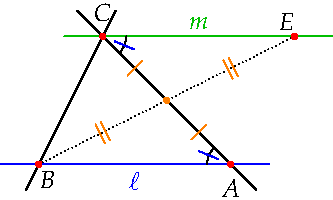
\includegraphics{euclid-playfair3}
\end{minipage}\bigbreak

In fact the postulates are equivalent.

\begin{thm}{}{}
	In the presence of Euclid's first four postulates, Playfair's postulate and the parallel postulate (P5) are equivalent.
\end{thm}

\begin{proof}
	\begin{description}
		\item[\normalfont (P5 $\Rightarrow$ Playfair)] We proved this above.
		\item[\normalfont (Playfair $\Rightarrow$ P5)] We prove the contrapositive. Assume postulates P1--P4 are true and that P5 is \emph{false.} Using quantifiers, and with reference to the picture in I.\,29, we restate the parallel postulate:
	\begin{quote}
	  P5:\lstsp $\forall$ pairs of lines $\ell,m$ and $\forall$ crossing lines $n$, \  $\beta+\gamma<\ang{180}\implies\ell,m$ \emph{not parallel.}
	\end{quote}
	\begin{minipage}[t]{0.62\linewidth}\vspace{-7pt}
		Its \emph{negation} (P5 false) is therefore:
		\begin{quote}
	  	$\exists$ parallel lines $\ell,m$ and a crossing line $n$ for which $\beta+\gamma<\ang{180}$
		\end{quote}
		This is without loss of generality: if $\beta+\gamma>\ang{180}$, consider the angles on the other side of $n$.\medbreak
		By the the exterior angle theorem/I.\,28, we may build a parallel line $\hat\ell$ to $\ell$ through the intersection $C$ of $m$ and $n$: in the picture, $\hat\beta\cong\beta$. Crucially, this only requires postulates P1--P4!
	\end{minipage}
	\hfill
	\begin{minipage}[t]{0.37\linewidth}\vspace{0pt}
		\flushright
		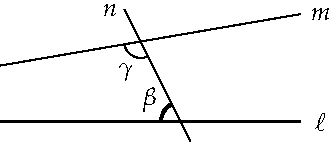
\includegraphics{euclid-playfair2}\\
		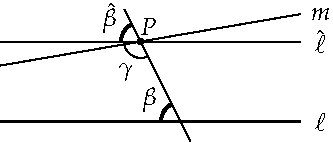
\includegraphics{euclid-playfair}
	\end{minipage}\smallbreak
	Observe that $\hat\ell$ and $m$ are \emph{distinct} since $\hat\beta+\gamma\cong\beta+\gamma<\ang{180}$.
	We therefore have a line $\ell$ and a point $C$ not on $\ell$, though which pass (at least) \emph{two} parallels to $\ell$: Playfair's postulate is \emph{false.} \qedhere
	\end{description}
\end{proof}



\boldsubsubsection{Non-Euclidean Geometry}\phantomsection\label{pg:sphere}

That Euclid waited so long before invoking the uniqueness of parallels suggests he was trying to establish as much as he could about triangles and basic geometry in its absence. By contrast, everything from I.\,29 onwards relies on the parallel postulate, including the proof that the angle sum in a triangle is \ang{180}. For centuries, many mathematicians believed, though none could prove it, that such a fundamental fact about triangles must be true independent of the parallel postulate.\smallbreak
Loosely speaking, a \emph{non-Euclidean geometry} is a model for which a parallel through an off-line point either doesn't exist or is non-unique. It wasn't until the 17--1800s and the development of \emph{hyperbolic geometry} (Chapter \ref{chap:hyper}) that a model was found in which Euclid's first four postulates hold but for which the parallel postulate is false.\footnote{This shows that the parallel postulate is independent: in fact all Euclid's postulates are independent. They are also consistent (the `usual' points and lines in the plane are a model), but incomplete: a sample undecidable is in Exercise \ref{ex:euclidundecideable}.}\par

\begin{minipage}[t]{0.76\linewidth}\vspace{-5pt}
	We shall eventually see that every triangle in hyperbolic geometry has angle sum less than \ang{180}, though this will require a lot of work! For a more easily visualized non-Euclidean geometry consider the sphere. A rubber band stretched between three points on its surface describes a \emph{spherical triangle}; an example with angle sum \ang{270} is drawn. A similar game can be played on a saddle-shaped surface: as in hyperbolic geometry, `triangles' will have angle sum less than \ang{180}.
\end{minipage}
\hfill
\begin{minipage}[t]{0.23\linewidth}\vspace{-10pt}
	\flushright
	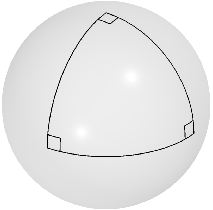
\includegraphics[scale=0.95]{euclid-sphere}
\end{minipage}

\goodbreak

\goodbreak


\boldsubsubsection{Pythagoras' Theorem}

Following his discussion of parallels, Euclid shows that parallelograms with the same base and height are equal (in area) (I.\,33--41), before providing constructions of parallelograms and squares (I.\,42--46). Some of this is in Exercise \ref{ex:pythagexs}. Immediately afterwards comes the capstone of Book I.


\begin{thm}{I.\,47 Pythagoras' Theorem}{}
	The square on the hypotenuse of a right triangle equals (has the same area as) the sum of the squares on the other sides.
\end{thm}

\begin{proof} 
	The given triangle $\triangle ABC$ is assumed to have a right-angle at $A$.\par
	\begin{minipage}[t]{0.6\linewidth}\vspace{0pt}
	\begin{enumerate}\itemsep0pt
	  \item Construct squares on each side of $\triangle ABC$ \ (I.\,46) and a parallel $\cl{AL}$ to $\cl{BD}$ \ (I.\,16).
	  \item $\cl{AB}\cong\cl{FB}$ and $\cl{BD}\cong\cl{BC}$ since sides of squares are congruent. Moreover $\angle ABD\cong\angle FBC$ since both contain \textcolor{blue}{$\angle ABC$} and a \textcolor{red}{right-angle}.
	  \item Side-angle-side (I.\,4) says that $\triangle ABD$ and $\triangle FBC$ are congruent (identical up to rotation by \ang{90}).
		\item I.\,41 compares areas of parallelograms and triangles with the same base and height:\vspace{0pt}
		\begin{align*}
			\operatorname{Area}(\textcolor{red}{\square ABFG})&=2\operatorname{Area}(\triangle FBC)\\
			&=2\operatorname{Area}(\triangle ABD)\\
			&=\operatorname{Area}\left(\textcolor{red}{\fbox{\phantom{'}}BOLD}\right)\\[-25pt]
		\end{align*}
		\item Similarly $\operatorname{Area}(\textcolor{Green}{\square ACKH}) =\operatorname{Area}\left(\textcolor{Green}{\fbox{\phantom{'}}OCEL}\right)$.
	\end{enumerate}
	\end{minipage}
	\hfill
	\begin{minipage}[t]{0.39\linewidth}\vspace{0pt}
		\flushright
		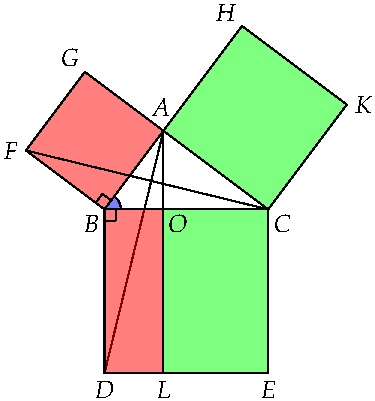
\includegraphics{euclid-I47}
	\end{minipage}
	\begin{enumerate}\setcounter{enumi}{5}
		\item Sum the rectangles to obtain $\square BCED$ and complete the proof.\hfill\qedhere
	\end{enumerate}
\end{proof}



Euclid finishes Book I with the converse, which we state without proof. Euclid's argument is very sneaky: look it up!

\begin{thm}{I.\,48}{}
	If the (areas of the) squares on two sides of a triangle equal the (area of the) square on the third side, then the  triangle has a right-angle opposite the third side.
\end{thm}

The \emph{Elements} contains thirteen books. Much of the remaining twelve discuss further geometric constructions, including in three dimensions. There is also a healthy dose of basic number theory including what is now known as the Euclidean algorithm.\medbreak

While undoubtedly a masterpiece of logical reasoning, Euclid's presentation has several flaws. Most problematic is his reliance on pictorial reasoning: for instance he `proves' the SAS and SSS congruence theorems (I.\,4 \& 8) by laying one triangle on top of another, a process not justified by his axioms (look it up \href{http://math.furman.edu/~jpoole/euclidselements/euclid.htm}{online} or \href{http://math.uci.edu/~ndonalds/Elements-I-VI.pdf}{Byrne}). In a modern sense, Euclid's approach is part axiomatic system and part model: his reasoning requires a visual/physical representation of lines, circles, etc. Because of these issues, we now turn to a more modern description of Euclidean geometry, courtesy of David Hilbert.

\clearpage

% 
% \paragraph{Book II: Geometric algebra}
% 
% We tend to think of Pythagoras' Theorem as a statement in Geometric Algebra: i.e., $c^2=a^2+b^2$, but this is not how Euclid saw it. To Euclid, Geometric Algebra was about solving equations to find unknowns. Of course the concept of algebra hadn't been invented yet, so the very problems had to be stated geometrically. Such concerns comprise the bulk of Book II of the \emph{Elements,} and are mostly attributable to the Pythagoreans.Here is an example.
% 
% \begin{thm*}[II.\,11]
% A straight line can be divided so that the rectangle contained by the whole and one of the segments is equal to the square on the remaining segment.
% \end{thm*}
% 
% 
%  In our modern language we would say: given $AB=a$, find $H$ on $AB$, so that $AH=x$, with $x^2=a(a-x)$. Here is Euclid's proof.
% 
% \begin{minipage}{0.3\textwidth}
% 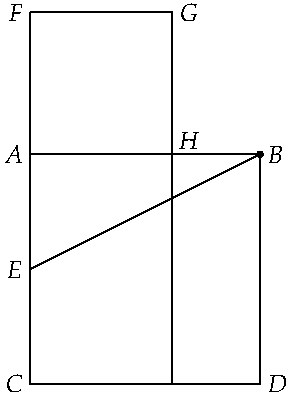
\includegraphics{geo-17-bk2}
% \end{minipage}\hfill
% \begin{minipage}{0.6\textwidth}
% \begin{enumerate}
%   \item Construct square $ABDC$ on $AB$
% 	\item Bisect $AC$; call midpoint $E$
% 	\item Connect $EB$
% 	\item Extend $AC$
% 	\item Lay off $EF=EB$ on $AC$ extended
% 	\item Construct square $FGHA$
% \end{enumerate}
% \end{minipage}
% 
%  In our modern language, with our understanding of Pythagoras', we see that Euclid has constructed $H$ so that $x=\frac{\sqrt 5-1}2a$. We can easily check that this solves the equation $x^2=a(a-x)$. Note that this is a construction of the golden ratio:
% \[AH:HB=1:\frac{\sqrt 5-1}2=\frac{\sqrt 5+1}2:1.\]
% For many centuries after Euclid, the meaning of `solve' was exactly this: construct a solution.


\begin{exercises}
	\hangindent\doubleind
	1. \ (a) \ Prove the \emph{vertical angle theorem} (I.\,15): if two lines cut one another, opposite angles are congruent.\vspace{-8pt}

	\begin{enumerate}\setcounter{enumi}{1}
	  \item[]\begin{enumerate}\setcounter{enumii}{1}
	    \item[](\emph{Hint: This is one place where you will need to use postulate 4 regarding right-angles})
	    \item Use part (a) to complete the proof of the exterior angle theorem: i.e.\ explain why $\beta<\delta$.
	  \end{enumerate}
	
		\item\label{ex:pythagexs} To help prove Pythagoras', Euclid makes use of the following results. Prove them as best as you can: full rigor is tricky, but the pictures should help!
		\begin{enumerate}
		  \item (I.\,11) At a given point on a line, to construct a perpendicular.
		  \item (I.\,46) To construct a square on a given segment.
		  \item (I.\,35) Parallelograms on the same base and with the same height have equal area.
		  \item (I.\,41) A parallelogram has twice the area of a triangle on the same base and with the same height.
		\end{enumerate}
		
		\begin{center}
			\begin{tabular}{c@{\quad}c@{\quad}c}
				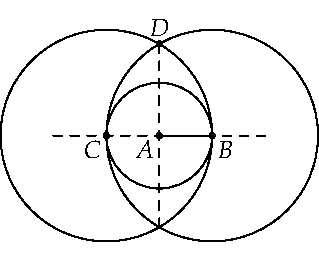
\includegraphics[scale=0.95]{euclid-I11}
				&
				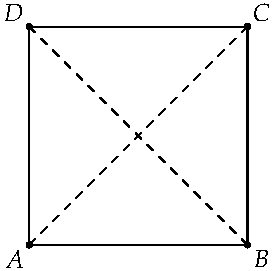
\includegraphics[scale=0.95]{euclid-I46}
				&
				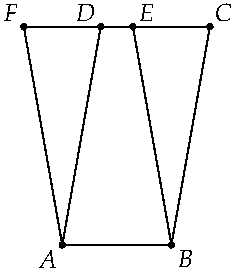
\includegraphics[scale=0.95]{euclid-I35a}
				\\[-2pt]
				Theorem I.\,11
				&
				Theorem I.\,46
				&
				Theorem I.\,35
			\end{tabular}
		\end{center}
		
	  
	  \item Consider spherical geometry (page \pageref{pg:sphere}), where \emph{lines} are paths of shortest distance (great circles).
	 	\begin{enumerate}
	 	  \item Which of Euclid's postulates P1--P5 are satisfied by this geometry?
	  	\item (Hard)\lstsp Where does the proof of the exterior angle theorem \emph{fail} in spherical geometry? 
	 	\end{enumerate}
	  
	  
	  \item\begin{enumerate}
	    \item State the negation of Playfair's postulate.
	    \item Prove that Playfair's postulate is equivalent to the following statement:
	  \begin{quote}
	  	Whenever a line is perpendicular to one of two parallel lines, it must be perpendicular to the other.
	  \end{quote}
	  \end{enumerate}
	 
	  
	  \item\label{ex:euclidundecideable} The \emph{line-circle continuity} property states:
	  \begin{quote}
	  If point $P$ lies inside and $Q$ lies outside a circle $\alpha$, then the segment $\overline{PQ}$ intersects $\alpha$.
	  \end{quote}
	  By considering the set of rational points in the plane $\Q^2=\{(x,y):x,y\in\Q\}$, and making a sensible definition of line and circle, show that the line-circle continuity property is undecidable within Euclid's system.
		
		
		\item The standard proof of the converse of Pythagoras' theorem (I.\,48) is, in fact, a \emph{corollary} of the original! Look it up and explain the argument as best you can.
	\end{enumerate}
	
\end{exercises}

\clearpage



\subsection{Hilbert's Axioms I: Incidence and Order}\label{sec:hilbert1}

The long process of identifying and correcting the errors and omissions in Euclid's \emph{Elements} culminated in the 1899 publication of David Hilbert's \emph{Grundlagen der Geometrie (Foundations of Geometry)}. In the next two sections we consider some of the details of Hilbert's approach, providing a modern and logically superior description of Euclidean geometry.\smallbreak

Hilbert's axioms for plane geometry\footnote{Like Euclid, Hilbert also covered 3D geometry; we only give the axioms for plane geometry. With regard to our desired properties (Definition \ref{defn:consistency}), his system is about as good as can be hoped. Essentially one only one model exists, which is almost the same thing as completeness. In the absence of the continuity axiom, the axioms are consistent; in line with Gödel's theorems (\ref{thm:godel}), consistency cannot be proved once continuity is included. As stated, the axioms are not quite independent, though this can be remedied: O-3 does not require existence (follows from Pasch's axiom), C-1 does not require uniqueness (follows from uniqueness in C-4) and C-6 can be weakened slightly.} are listed on the next page. The undefined terms consist of two types of object (\emph{points} and \emph{lines}), and three relations (\emph{between $*$, on $\in$} and \emph{congruence $\cong$}). For brevity we'll often use/abuse set notation, viewing a line as a set of points, though this is not necessary. At various places, definitions and notations are required.

\begin{defn}{}{hilbertbasic}
	Throughout, $A,B,C$ denote points and $\ell,m$ lines.
	\begin{description}\itemsep 0pt plus 1pt
	  \item[\normalfont\emph{Line}:] $\smash[t]{\lin{AB}}$ denotes the line through distinct $A,B$. This exists and is unique by axioms I-1 and I-2.
	  \item[\normalfont\emph{Segment}:] $\cl{AB}:=\{A,B\}\cup\{C:A*C*B\}$ consists of distinct \emph{endpoints} $A,B$ and all \emph{interior} points $C$ lying between them.
	  \item[\normalfont\emph{Ray}:] $\ray{AB}:=\cl{AB}\cup\{C:A*B*C\}$ is a ray with \emph{vertex} $A$. In essence we extend $\cl{AB}$ beyond $B$.
	  \item[\normalfont\emph{Triangle}:] $\triangle ABC:=\cl{AB}\cup\cl{BC}\cup\cl{CA}$ where $A,B,C$ are non-collinear. Triangles are \emph{congruent} if their sides and angles are congruent in pairs.
		\item[\normalfont\emph{Sidedness}:] Distinct $A,B$, not on $\ell$, lie on the \emph{same side} of $\ell$ if $\cl{AB}\cap\ell=\emptyset$. Otherwise $A$ and $B$ lie on \emph{opposite sides} of $\ell$.
		\item[\normalfont\emph{Angle}:] $\angle BAC:=\ray{AB}\cup\ray{AC}$ has \emph{vertex} $A$ and \emph{sides} $\ray{AB}$ and $\ray{AC}$.
		\item[\normalfont\emph{Parallelism}:] Lines $\ell$ and $m$ \emph{intersect} if there exists a point lying on both: $\exists A\in\ell\cap m$. Lines are \emph{parallel} if they do not intersect. Segments/rays are parallel when the corresponding lines are parallel.
	\end{description}
	The pictures represent these notions in the usual model of Cartesian geometry.
	\begin{center}
		\begin{tabular}{@{}c@{\qquad}c@{\qquad}c@{\qquad}c@{}}
			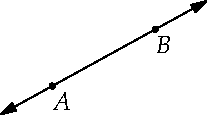
\includegraphics{hilbert-def-line}
			&
			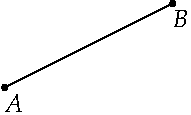
\includegraphics{hilbert-def-seg}
			&
			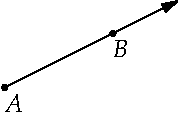
\includegraphics{hilbert-def-ray}
			&
			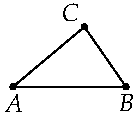
\includegraphics{hilbert-def-triangle}
			\\
			Line $\lin{AB}$
			&
			Segment $\cl{AB}$
			&
			Ray $\ray{AB}$
			&
			Triangle $\triangle ABC$
			\\[12pt]
			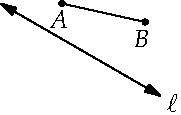
\includegraphics{hilbert-def-side}
			&
			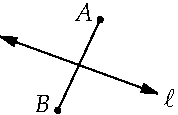
\includegraphics{hilbert-def-side2}
			&
			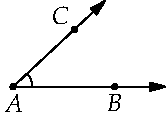
\includegraphics{hilbert-def-angle}
			&
			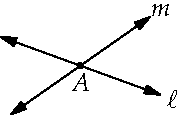
\includegraphics{hilbert-def-intersect}
			\\
			Same side
			&
			Opposite sides
			&
			Angle $\angle BAC$
			&
			Intersection $A\in\ell\cap m$
		\end{tabular}
	\end{center}
\end{defn}


\pagebreak
\thispagestyle{empty}
\begin{center}
\bfseries\Large Hilbert's Axioms for Plane Geometry
\end{center}

\begin{minipage}[t]{0.46\linewidth}
\boldinline{Undefined terms}
\begin{enumerate}\itemsep2pt
  \item \emph{Points}: \ use capital letters, $A,B,C\ldots$
  \item \emph{Lines}: \ use lower case letters, $\ell,m,n,\ldots$
  \item \emph{On}: \ $A\in\ell$ is read `$A$ lies on $\ell$'
  \item \emph{Between}: \ $A*B*C$ is read `$B$ lies between $A$ and $C$'
  \item \emph{Congruence}: \ $\cong$ is a binary relation on segments or angles
\end{enumerate}

\boldinline{Axioms of Incidence}

\begin{enumerate}
	\item[I-1] For any distinct $A,B$ there exists a line $\ell$ on which lie $A,B$.
	\item[I-2] There is at most one line through distinct $A,B$ \ ($A$ and $B$ both \emph{on} the line).
\end{enumerate}\vspace{-2pt}
	
Notation: \emph{line} $\overleftrightarrow{AB}$ through $A$ and $B$\vspace{-2pt}

\begin{enumerate}\setcounter{enumi}{2}	
	\item[I-3] On every line there exist at least two distinct points. There exist at least three points not all on the same line.
\end{enumerate}


\boldinline{Axioms of Order}

\begin{enumerate}
	\item[O-1] If $A*B*C$, then $A,B,C$ are distinct points on the same line and $C*B*A$.
	\item[O-2] Given distinct $A,B$, there is at least one point $C$ such that $A*B*C$.
	\item[O-3] If $A,B,C$ are distinct points on the same line, exactly one lies between the others.
\end{enumerate}\vspace{-2pt}
	
Definitions: \emph{segment} $\cl{AB}$ and \emph{triangle} $\triangle ABC$\vspace{-2pt}

\begin{enumerate}\setcounter{enumi}{3}	
	\item[O-4] (Pasch's Axiom) Let $\triangle ABC$ be a triangle and $\ell$ a line not containing any of $A,B,C$. If $\ell$ contains a point of the segment $\cl{AB}$, then it also contains a point of either $\cl{AC}$ or $\cl{BC}$. 
\end{enumerate}

Definitions: \emph{sides} of line $\overleftrightarrow{AB}$ and \emph{ray} $\ray{AB}$
\end{minipage}
\hfill
\begin{minipage}[t]{0.48\linewidth}
\boldinline{Axioms of Congruence}

\begin{enumerate}
  \item[C-1] (Segment transference) \ Let $A,B$ be distinct and $r$ a ray based at $A'$. Then there exists a unique point $B'\in r$ for which $\cl{AB}\cong\cl{A'B'}$. Moreover $\cl{AB}\cong\cl{BA}$.
  \item[C-2] If $\cl{AB}\cong\cl{EF}$ and $\cl{CD}\cong\cl{EF}$, then $\cl{AB}\cong\cl{CD}$.
  \item[C-3] If $A*B*C$, \ $A'*B'*C'$, \ $\cl{AB}\cong\cl{A'B'}$ and $\cl{BC}\cong\cl{B'C'}$, then $\cl{AC}\cong\cl{A'C'}$.
  \end{enumerate}
	
Definitions: \emph{angle} $\angle ABC$\vspace{-2pt}

\begin{enumerate}\setcounter{enumi}{3}
  \item[C-4] (Angle transference) \ Given $\angle BAC$ and $\ray{A'B'}$, there exists a unique ray $\ray{A'C'}$ on a given side of $\overleftrightarrow{A'B'}$ for which $\angle BAC\cong\angle B'A'C'$.
  \item[C-5] If $\angle ABC\cong\angle GHI$ and $\angle DEF\cong\angle GHI$, then $\angle ABC\cong\angle DEF$. Moreover, $\angle ABC\cong\angle CBA$.
  \item[C-6] (Side-angle-side) Given triangles $\triangle ABC$ and $\triangle A'B'C'$, if $\cl{AB}\cong\cl{A'B'}$, $\cl{AC}\cong\cl{A'C'}$, and $\angle BAC\cong\angle B'A'C'$, then the triangles are congruent.\footnotemark{}
\end{enumerate}

\boldinline{Axiom of Continuity}\phantom{bob}\smallbreak

Suppose $\ell$ is partitioned into non-empty subsets $\Sigma_1,\Sigma_2$ such that no point of $\Sigma_1$ lies between two points of $\Sigma_2$ and vice versa.\par
Then there exists a unique point $\mathcal O\in\ell$ satisfying $P_1*\mathcal O*P_2$, if and only if $\mathcal O\neq P_1$, $\mathcal O\neq P_2$ and one of $P_1$ or $P_2$ lies in $\Sigma_1$ and the other in $\Sigma_2$.\medbreak



\boldinline{Playfair's Axiom}\phantom{bob}\smallbreak

Definition: \emph{parallel lines}\smallbreak

Given a line $\ell$ and a point $P$ not on $\ell$, there exists at most one line through $P$ parallel to $\ell$.
\end{minipage}

\footnotetext{Its sides/angles are congruent in pairs. We extend congruence to other geometric objects similarly.}

\clearpage





\boldsubsubsection{Axioms of Incidence: Finite Geometries}

The axioms of incidence describe the relation \emph{on.} An \emph{incidence geometry} is any model satisfying axioms I-1, I-2, I-3. Perhaps surprisingly, there exist incidence geometries with \emph{finitely many points}!

\begin{examples}{}{fano}
	By I-3, an incidence geometry requires \emph{at least three} points.\par
	\begin{minipage}[t]{0.62\linewidth}\vspace{-5pt}
		A 3-point geometry exists, and is unique up to relabelling:\smallbreak
		I-3 says the points $A,B,C$ must be non-collinear. By I-1 and I-2, each pair lies on a unique line, whence there are precisely three lines
		\[
			\ell=\{A,B\},\quad m=\{A,C\},\quad n=\{B,C\}
		\]
		Up to relabelling, there are two incidence geometries with four points: one is drawn; how many lines has the other?
	\end{minipage}
	\hfill
	\begin{minipage}[t]{0.37\linewidth}\vspace{-15pt}
		\flushright
		\begin{tabular}{cc@{}}
			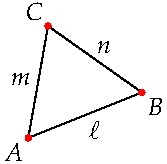
\includegraphics{hilbert-incidence3}
			&
			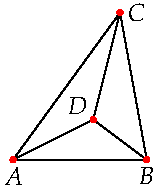
\includegraphics{hilbert-incidence4}\\
			3 points, 3 lines
			&
			%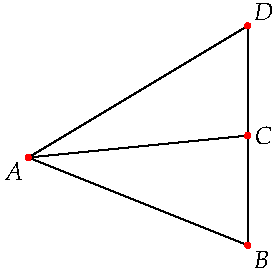
\includegraphics{hilbert-incidence4-2}
			4 points, 6 lines%&4 points, 4 lines
		\end{tabular}
	\end{minipage}
	\smallbreak
	\begin{minipage}[t]{0.72\linewidth}\vspace{0pt}
		The final picture is a famous example called the \emph{Fano plane,} an incidence geometry with seven points and seven lines, which finds many applications particularly in combinatorics. Each point lies on precisely three lines and each line contains precisely three points; each dot is colored to indicate the lines to which it belongs. Don't be fooled by the black line looking `curved' and seeming to cross the blue line near the top; it really only contains three points!
	\end{minipage}
	\hfill
	\begin{minipage}[t]{0.27\linewidth}\vspace{-17pt}
		\flushright
		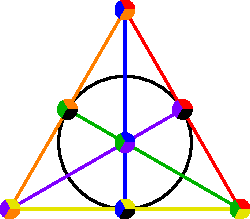
\includegraphics{hilbert-incidence7}
	\end{minipage}
\end{examples}

We can even prove some simple theorems in incidence geometry.

\begin{lemm}{}{intersectunique}
	If distinct lines intersect, then they do so in exactly one point.
\end{lemm}

\begin{proof}
	Suppose $A,B$ are distinct points of intersection. By axiom I-2, there is at most one line through $A$ and $B$. Contradiction.
\end{proof}

\begin{lemm}{}{incidenceeasy}
	Given any point, there exist at least two lines on which it lies.
\end{lemm}

The proof is an exercise. While incidence geometry is fun, our main goal is to understand Euclidean geometry, so we move on to the next set of axioms.


\boldsubsubsection{Axioms of Order: Sides of a Line, Pasch's Axiom \& the Crossbar Theorem}

The axioms of order describe the ternary relation \emph{between.} Their inclusion in Hilbert's axioms is due in no small part to the work of Moritz Pasch, after whom Pasch's axiom (O-4, c.\,1882) is named. This axiom is very powerful; in particular, it permits us to define the \emph{interiors} of several geometric objects, and to see that these are non-empty.

\begin{lemm}{}{seginterior}
	Every segment contains an interior point.
\end{lemm}

We leave the proof to Exercise \ref{exs:seginterior}. By inducting on the Lemma, every segment contains \emph{infinitely many} points, whence the above finite geometries are not valid models once the order axioms are included.

\goodbreak

To get much further, it is necessary to establish that a line has precisely two \emph{sides} (Definition \ref{defn:hilbertbasic}). This concept lies behind several of Euclid's arguments, without being properly defined in the \emph{Elements.}


\begin{thm}{Plane Separation}{planesep}
	A line $\ell$ separates all points not on $\ell$ into two half-planes; the two \emph{sides} of $\ell$. Explicitly: suppose none of the points $A,B,C$ lie on $\ell$, then:
	\begin{enumerate}\itemsep0pt
	  \item If $A,B$ lie on the same side of $\ell$ and $B,C$ lie on the same side, then $A,C$ lie on the same side.
	  \item If $A,B$ lie on opposite sides and $B,C$ lie on opposite sides, then $A,C$ lie on the same side.
	  \item If $A,B$ lie on opposite sides and $B,C$ lie on the same side, then $A,C$ lie on opposite sides.
	\end{enumerate}\vspace{-10pt}
	\begin{center}
		\begin{tabular}{c@{\qquad}c@{\qquad}c}
			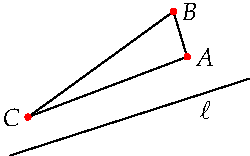
\includegraphics{hilbert-planesep}
			&
			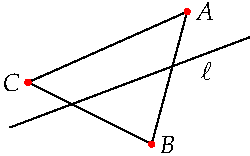
\includegraphics{hilbert-planesep2}
			&
			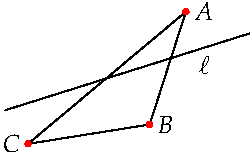
\includegraphics{hilbert-planesep3}
			\\
			Case 1
			&
			Case 2
			&
			Case 3
		\end{tabular}
	\end{center}
\end{thm}

\begin{proof}
	We prove the contrapositive of case 1. Suppose $A,B,C$ are non-collinear. If $\cl{AC}$ intersects $\ell$, then $\ell$ intersects one side of $\triangle ABC$. By Pasch's axiom, it also intersects either $\cl{AB}$ or $\cl{BC}$.\smallbreak
	The other cases are exercises, and we omit the tedious collinear possibilities.
\end{proof}

Plane separation/sidedness allows us to properly define interiors of angles and triangles. 

\begin{defn}{}{interiorangle}
	A point $I$ is \emph{interior} to angle $\angle BAC$ if:\par
	\begin{minipage}[t]{0.6\linewidth}\vspace{0pt}
		\begin{itemize}\itemsep0pt
	  	\item $I$ lies on the same side of $\lin{AB}$ as $C$, and,
	  	\item $I$ lies on the same side of $\lin{AC}$ as $B$.
		\end{itemize}
		Otherwise said, $I$ lies in the intersection of two half-planes.
	\end{minipage}
	\hfill
	\begin{minipage}[t]{0.35\linewidth}\vspace{-20pt}
		\flushright
		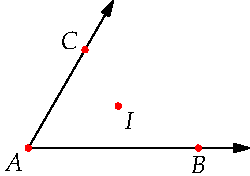
\includegraphics[scale=0.95]{hilbert-interior}
	\end{minipage}\medbreak
	
	A point $I$ is \emph{interior} to triangle $\triangle ABC$ if it is interior to all three of its angles $\angle ABC$, $\angle BAC$ and $\angle ACB$. Otherwise said, $I$ lies in the triple intersection of three of the half-planes defined by the triangle's sides.
\end{defn}

Interior points permit us to compare angles: if $I$ is interior to $\angle BAC$, then $\angle BAI<\angle BAC$ has obvious meaning, \emph{without resorting to numerical angle measure.}

\begin{cor}{}{angleinteriorexist}
	Every angle has an interior point.
\end{cor}

\begin{proof}
	Given $\angle BAC$, consider any interior point $I$ of the segment $\cl{BC}$. This plainly lies on the same side of $\lin{AB}$ as $C$ and on the same side of $\lin{AC}$ as $B$.
\end{proof}

In Exercise \ref{exs:seginfinite}, we check that the interior of a triangle is non-empty.
\vfil

\goodbreak
%\medbreak

Pasch's axiom could be paraphrased as follows: \emph{If a line enters a triangle, it must come out.} We haven't quite established this crucial fact however. What if the line passes through a vertex?

\goodbreak
 
\begin{thm}[lower separated=false, sidebyside, sidebyside align=top seam, sidebyside gap=0pt, righthand width=0.3\linewidth]{Crossbar Theorem}{}
	Suppose $I$ is interior to $\angle BAC$. Then $\ray{AI}$ intersects $\cl{BC}$.\medbreak
In particular, if a line passes through a vertex and an interior point of a triangle, then it intersects the side opposite the vertex.
	\tcblower
	\flushright
	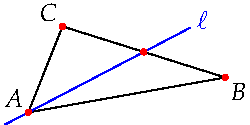
\includegraphics{hilbert-pasch2}
\end{thm}


\begin{proof}
	Extend $\cl{AB}$ to a point $D$ such that $A$ lies between $B$ and $D$ (O-2). Since $C$ is not on $\lin{BD}=\lin{AB}$ we have a triangle $\triangle BCD$. Since $\lin{AI}$ intersects one edge of $\triangle BCD$ at $A$ and does not cross any vertices (think about why\ldots), Pasch says it intersects one of the other edges ($\cl{BC}$ or $\cl{CD}$) at some point $M$.\smallbreak
	The result follows from applying plane separation to the lines $\lin{AB}=\lin{BD}$ and $\lin{AC}$. First observe:
	\begin{quote}
		Since $I,M$ lie on the same side of $\smash{\lin{AB}=\lin{BD}}$ as $C$, it follows that $\smash{\cl{IM}}$ does not intersect $\smash{\lin{AB}}$. Since $A,I,M$ are collinear and $A\in\lin{AB}$, it follows that \textcolor{red}{$A\notin\cl{IM}$}.
	\end{quote}
	If $M\in\cl{BC}$, we are done. Our goal is to show that $M\in\cl{CD}$ is a contradiction.\vspace{-5pt}
	\begin{center}
		\begin{tabular}{cc}
			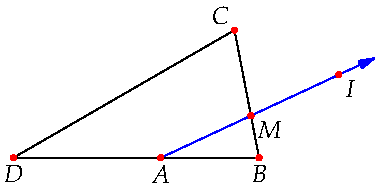
\includegraphics[scale=0.95]{hilbert-crossbar1}
			&
			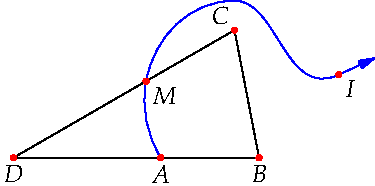
\includegraphics[scale=0.95]{hilbert-crossbar2}
			\\
			correct arrangement\footnotemark{}
			&
			contradiction
		\end{tabular}
	\end{center}
	Suppose, for contradiction, that $M\in\cl{CD}$. Relative to $\lin{AC}$:
	\begin{itemize}\itemsep0pt
		  \item $I$ and $B$ lie on the same side since $I$ is interior to $\angle BAC$;
		  \item $B$ and $D$ lie on opposite sides, since $B*A*D$ and $\lin{AC}\neq\lin{BD}=\cl{AB}$;
		  \item $D$ and $M$ lie on the same side since $M\in\cl{CD}$ and $\lin{CD}\neq\lin{AC}$.		  
	\end{itemize}
	By plane separation, $I,M$ lie on opposite sides of $\lin{AC}$. The collinearity of $A,I,M$ then forces the contradiction \textcolor{red}{$A\in\cl{IM}$}.
\end{proof}

\footnotetext{The pictures could be modified: e.g., $I=M$ and $A*I*M$ are also correct arrangements ($M\in\cl{BC}$).}


\begin{minipage}[t]{0.67\linewidth}\vspace{-8pt}
	Euclid repeatedly uses the crossbar theorem without justification, including in his construction of perpendiculars and angle/segment bisectors (Theorems I.\,9+10). We sketch the latter here.\smallbreak
	Given $\angle BAC$, construct $E$ such that $\cl{AB}\cong\cl{AE}$. Construct $D$ using an equilateral triangle (I.\,1). SSS (I.\,8) shows that $\angle BAC$ is bisected, and SAS (I.\,4) that $\ray{AD}$ bisects $\cl{BE}$.\smallbreak
	Quite apart from Euclid's arguments for SAS and SSS being suspect (we'll deal with these in the next section), he gives no argument for why $D$ is interior to $\angle BAC$ or why $\ray{AD}$ should intersect $\cl{BE}$!
\end{minipage}
\hfill
\begin{minipage}[t]{0.32\linewidth}\vspace{0pt}
	\flushright
	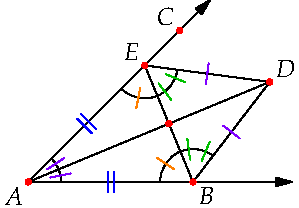
\includegraphics{hilbert-bisect}
\end{minipage}
\medbreak


Even with Pasch's axiom and the crossbar theorem, it requires some effort to repair Euclid's proof. No matter; we'll provide an alternative construction of the bisector once we've considered congruence.

\goodbreak


\begin{exercises}
	\exstart Label the vertices in the Fano plane 1 through 7 (any way you like). As we did in Example \ref{ex:fano} for the 3-point geometry, describe each line in terms of its points.
	\begin{enumerate}\setcounter{enumi}{1}
	  \item Prove Lemma \ref{lemm:incidenceeasy}.
	  
	  
	  \item Give a model for each of the 5-point incidence geometries: how many are there?\par
	  (\emph{Hint: remember that order doesn't matter, so the only issue is how many points lie on each line})
	  
	    
	  \item Consider the proof of the crossbar theorem. Explain how we know that $\smash[t]{\lin{AI}}$ does not contain any of the vertices of $\triangle BCD$.
	  
	  
	  \item\label{exs:seginterior} You are given distinct points $A,B$. Using the axioms of incidence and order and Lemma \ref{lemm:intersectunique} (follows from I-2), show the existence of each of the points $C,D,E,F$ in the picture \emph{in alphabetical order.} Hence conclude the existence of a point $F$ lying \emph{between} $A$ and $B$ (Lemma \ref{lemm:seginterior}).\par
	  \begin{minipage}[t]{0.65\linewidth}\vspace{-5pt}
	  During your construction, address the following issues:
	  \begin{enumerate}\itemsep0pt
	    \item Explain why $D$ does not lie on $\overleftrightarrow{AB}$.
			\item Explain why $E$ does not lie on $\triangle ABD$.
			\item Explain why $E\neq C$ (whence $\overleftrightarrow{CE}$ exists).
			\item Explain why $F$ lies on $\cl{AB}$ and \emph{not} on $\cl{BD}$.
		\end{enumerate}
	  \end{minipage}
	  \hfill
	  \begin{minipage}[t]{0.34\linewidth}\vspace{-5pt}
	  	\flushright
	  	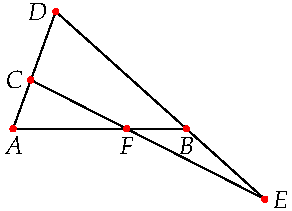
\includegraphics[scale=0.9]{hilbert-between}
	  \end{minipage}
	  
	  
	  \item\label{exs:bernays} We complete the proof of the plane separation theorem (\ref{thm:planesep}).
	  \begin{enumerate}
	    \item Prove part 3 (it is almost a verbatim application of Pasch's axiom).\par
	    \begin{minipage}[t]{0.75\linewidth}\vspace{-5pt}
	    \item Suppose a line $\ell$ intersects all three sides of $\triangle ABC$ but no vertices. This results in a very strange picture: we've labelled the intersections $D,E,F$ and WLOG chosen $D*E*F$.\smallbreak
	    Apply Pasch's axiom to $\triangle DBF$ and $\lin{AC}$ to obtain a contradiction. Hence establish part 2 of the plane separation theorem.    
	    \end{minipage}
	    \hfill
	    \begin{minipage}[t]{0.24\linewidth}\vspace{-35pt}
	    	\flushright
	    	\includegraphics{hilbert-bernays}
	    \end{minipage}
	  \end{enumerate}
	  
	  
	  \item Suppose $A,B,C$ are distinct points on a line $\ell$.
	  \begin{enumerate}
	    \item Explain why there exists a line $m\neq \ell$ such that $B\in m$.
	    \item Prove that $A*B*C\iff A$ and $C$ lie on opposite sides of $m$.
	    \item Suppose $A*B*C$. Use part (b) to prove the following:
	    \begin{enumerate}
				\item $B$ is the only point common to the rays $\ray{BA}$ and $\ray{BC}$.
				\item If $D\in\ell$ is any point other than $B$, prove that $D$ lies in precisely one of $\ray{BA}$ or $\ray{BC}$.
			\end{enumerate}
	  \end{enumerate}
	  
	  
	  \item\label{exs:seginfinite} Prove that the interior of a triangle is non-empty.\par
	  (\emph{Hint: use Exercise \ref{exs:seginterior} to construct a suitable $I$, then prove that it lies on the correct side of each edge})
	  
	\end{enumerate}
\end{exercises}


\clearpage



\subsection{Hilbert's Axioms II: Congruence}\label{sec:hilbert2}

Hilbert's congruence axioms address two primary issues in Euclid.
\begin{enumerate}
  \item Euclid's use of \emph{equal} is confusing. In Hilbert, segments/angles are now equal only when they are precisely the same (this amounts to the \emph{reflexivity} part of the next result).
  \item Euclid's frequent and unjustified use of pictorial reasoning. We previously discussed Euclid's erroneous approach to the SAS and SSS triangle congruence theorems. It was eventually realized that one of the triangle congruences has to be an axiom: SAS is Hilbert's C-6.
\end{enumerate}

We start with a small piece of bookkeeping.

\begin{lemm}{}{}
	Congruence of segments/angles is an equivalence relation.
\end{lemm}

\begin{proof}
	\begin{description}\itemsep0pt
  	\item[\normalfont(\emph{Reflexivity})] Let $\cl{AB}$ be given. Apply C-1 to obtain %\footnote{You could even take $A'=A$ and use the ray $r=\ray{AB}$!}
  	$\cl{A'B'}$ such that $\cl{AB}\cong\cl{A'B'}$. We sneakily use this \emph{twice} and apply C-2 to obtain
  	\[
  		\cl{AB}\cong\cl{A'B'}\text{ and } \cl{AB}\cong\cl{A'B'}\implies \cl{AB}\cong\cl{AB}
  	\]
  	\item[\normalfont(\emph{Symmetry})] Assume $\cl{AB}\cong\cl{CD}$. By reflexivity, $\cl{CD}\cong\cl{CD}$. By C-2 we have $\cl{CD}\cong\cl{AB}$.
  	\item[\normalfont(\emph{Transitivity})] Suppose $\cl{AB}\cong\cl{CD}$ and $\cl{CD}\cong\cl{EF}$. By symmetry, $\cl{EF}\cong\cl{CD}$. Axiom C-2 now shows that $\cl{AB}\cong\cl{EF}$.
  \end{description}
  \medskip
  Axioms C-4 and C-5 say essentially the same thing for angles (see Exercise \ref{exs:angcongequivrel}).
\end{proof}


\boldsubsubsection{Segment/Angle Transfer and Comparison}

Hilbert's axioms of segment and angle transference are crucial for comparing non-collinear segments and angles with distinct vertices.


\begin{defn}[lower separated=false, sidebyside, sidebyside align=top seam, sidebyside gap=0pt, righthand width=0.35\linewidth]{}{lengthcomp}
	Let segments $\cl{AB}$ and $\cl{CD}$ be given.\smallbreak
	By axiom C-1, let $E$ be the unique point on $\ray{CD}$ such that $\cl{CE}\cong\cl{AB}$: we have now \emph{transferred} $\cl{AB}$ onto $\ray{CD}$.\smallbreak
	We write $\cl{AB}<\cl{CD}$ if $E$ lies between $C$ and $D$, etc.
	\tcblower
	\flushright
	\includegraphics[scale=0.95]{angles-compare}
\end{defn}

By O-3, any two segments are comparable: given $\cl{AB}$ \& $\cl{CD}$, precisely one of the following holds,
\[
	\cl{AB}<\cl{CD}, \qquad \cl{CD}<\cl{AB}, \qquad\cl{AB}\cong\cl{CD}
\]
C-3 says that congruence respects the `addition' of adjacent congruent segments. Unique angle transfer, comparison and addition follow similarly from axiom C-4 and Definition \ref{defn:interiorangle} (interior points).\smallbreak

It is important to appreciate that neither Hilbert nor Euclid use or require an \emph{absolute} notion of length/angle-measure: $\cl{AB}<\cl{CD}$ does \emph{not} indicate a relationship between two numerical quantities (the \emph{lengths} of $\cl{AD}$ and $\cl{CD}$). Introducing length as a numerical quantity requires the inclusion of the real numbers (and thus far more axioms); for purity reasons, we postpone this until Section \ref{sec:similar}.
 

\goodbreak

\boldsubsubsection{The Triangle Congruence Theorems: SAS, ASA, SSS \& SAA}

Hilbert assumes side-angle-side (SAS) and proceeds to prove the remainder. Here is the first of these; we'll cover SSS momentarily and SAA in Exercise \ref{exs:saaproof}.

\begin{thm}{Angle-Side-Angle/ASA, Euclid I.\,26, case I}{asa}
	Suppose $\triangle ABC$ and $\triangle DEF$ satisfy
	\[
		\textcolor{Magenta}{\angle ABC}\cong\textcolor{Magenta}{\angle DEF},\qquad \textcolor{blue}{\cl{AB}}\cong\textcolor{blue}{\cl{DE}},\qquad \textcolor{red}{\angle BAC}\cong\textcolor{red}{\angle EDF}
	\]
	Then the triangles are congruent \ ($\angle ACB\cong\angle DFE$, \ $\cl{AC}\cong\cl{DF}$ and $\cl{BC}\cong\cl{EF}$).
\end{thm}

%We aren't (yet!) assuming uniqueness of parallels, so we cannot assert $\angle ACB\cong\angle DFE$.

Hilbert's approach modifies Euclid's; instead of laying $\triangle ABC$ on top of $\triangle DEF$, he creates a new triangle $\triangle DEG\cong \triangle ABC$ and proves that $G=F$.

\begin{proof}
	Segment transfer provides the unique point $G\in \ray{EF}$ such that $\textcolor{Green}{\cl{EG}}\cong \textcolor{Green}{\cl{BC}}$.\par
	\begin{minipage}[t]{0.65\linewidth}\vspace{0pt}
		SAS applied to $\textcolor{blue}{\cl{AB}}\cong\textcolor{blue}{\cl{DE}}$, $\textcolor{Magenta}{\angle ABC}\cong\textcolor{Magenta}{\angle DEG}\, (=\textcolor{Magenta}{\angle DEF})$, $\textcolor{Green}{\cl{BC}}\cong \textcolor{Green}{\cl{EG}}$, says $\textcolor{red}{\angle BAC}\cong \textcolor{red}{\angle EDG}\, (\cong \textcolor{red}{\angle EDF}$) (this last is by assumption).\smallbreak
		Since $F$ and $G$ lie on the same side of $\lin{DE}$, angle transfer (C-4) says they lie on the \emph{same ray} through $D$.\smallbreak
		But then $F$ and $G$ both lie on two distinct lines ($\lin{EF}=\lin{EG}$ and $\lin{DF}=\lin{DG}$); we conclude that $F=G$.\smallbreak
		By SAS we conclude that $\triangle ABC\cong\triangle DEF$.
	\end{minipage}
	\hfill
	\begin{minipage}[t]{0.34\linewidth}\vspace{-28pt}
		\flushright
		\includegraphics[scale=0.95]{angles-asa}
	\end{minipage}
\end{proof}




\boldsubsubsection{Geometry Without Circles}

Circles are at the heart of Euclid's constructions. Yet, for reason we'll address in Section \ref{sec:circ}, Hilbert essentially ignores them. We sketch a few of his alternative approaches to Euclid's basic results.

\begin{thm}{Euclid I.\,5}{euclidiso}
	An isosceles triangle has congruent base angles.
\end{thm}

Isosceles means \emph{equal legs}: two sides of the triangle are congruent. The remaining side is the \emph{base.} Euclid's argument relies on a famously complicated construction (look it up!). Hilbert does things more speedily and sneakily, by relabelling the original triangle and applying SAS.

\begin{tcolorbox}[proofstyle]
	\begin{minipage}[t]{0.7\linewidth}\vspace{0pt}
		\emph{Proof.}\lstsp Suppose $\triangle ABC$ is isosceles where $\textcolor{blue}{\cl{AB}}\cong\textcolor{blue}{\cl{AC}}$. Consider a `new' triangle $\triangle A'B'C'=\triangle ACB$ where the base points are switched:
		\[
			A':=A,\qquad B':=C,\qquad C':=B
		\]
		Observe:
		\begin{itemize}
		  \item $\textcolor{Green}{\angle BAC}\cong\textcolor{Green}{\angle CAB}$ (axiom C-5) $\implies\textcolor{Green}{\angle BAC}\cong\textcolor{Green}{\angle B'A'C'}$.
		  \item $\textcolor{blue}{\cl{AB}}\cong\textcolor{blue}{\cl{AC}}\implies \textcolor{blue}{\cl{AB}}\cong\textcolor{blue}{\cl{A'B'}}$ and $\textcolor{blue}{\cl{AC}}\cong\textcolor{blue}{\cl{A'C'}}$.
		\end{itemize}
		SAS says that $\angle ABC\cong\angle A'B'C'\cong\angle ACB$.
	\end{minipage}
	\hfill
	\begin{minipage}[t]{0.29\linewidth}\vspace{0pt}
		\flushright
		\includegraphics{angles-isos2}\\[-8pt]
		\hfill\qedsymbol
	\end{minipage}
\end{tcolorbox}


\goodbreak


\boldinline{Dropping a Perpendicular}

As with the majority of Book I, Euclid accomplishes this using circle intersections.\footnote{Consider the picture for Thm.\,I.\,11 in Exercise \ref*{sec:hilbert1}.\ref{ex:pythagexs}.} Hilbert instead uses segment/angle transference and the concept of sidedness.\par
	
\begin{minipage}[t]{0.69\linewidth}\vspace{0pt}
	Suppose we are given a line $\ell$ and a point $P$ not on $\ell$. Our goal is to construct a point $M\in\ell$ such that $\cl{PM}$ intersects $\ell$ in a right-angle.\smallbreak
	Let $A,B$ be distinct points on $\ell$ (axiom I-3) so that $\ell=\lin{AB}$.\smallbreak
	By axioms C-4 and C-1, we may transfer \textcolor{blue}{$\cl{AP}$} to the other side of $\ell$ at $A$, creating a new point $Q$.\smallbreak
	Since $P$ and $Q$ lie on opposite sides of $\ell$, the line intersects $\cl{PQ}$ at some point $M$. There are two cases to consider.
	\begin{itemize}
	  \item In the generic case $M\neq A$ (pictured), SAS applied to $\triangle MAP$ and $\triangle MAQ$ shows that $\angle AMP\cong\angle AMQ$. Since these angles sum to a straight edge ($\cl{PQ}$), they are both right-angles.
	  \item	In the extreme case $M=A$, there are no triangles and SAS cannot be applied. Instead, observe that $B$ does not lie on $\cl{PQ}$ (which axioms/results make this clear?!) and apply the above argument with $B$ instead of $A$.
	\end{itemize}
\end{minipage}
\hfill
\begin{minipage}[t]{0.29\linewidth}\vspace{0pt}
	\flushright
	\includegraphics[scale=1]{angles-perp}
\end{minipage}
\bigbreak

A generalization of this construction facilitates a corrected argument for the SSS triangle congruence.

\begin{thm}{Side-Side-Side/SSS, Euclid I.\,8}{}
	Suppose $\triangle ABC$ and $\triangle DEF$ have sides congruent in pairs:
	\[
		\textcolor{Magenta}{\cl{AB}}\cong\textcolor{Magenta}{\cl{DE}},\qquad \textcolor{violet}{\cl{BC}}\cong\textcolor{violet}{\cl{EF}},\qquad \textcolor{blue}{\cl{AC}}\cong\textcolor{blue}{\cl{DF}}
	\]
	Then the triangles are congruent ($\angle ABC\cong\angle DEF$, $\angle BCA\cong\angle EFD$, $\angle CAB \cong\angle FDE$).
\end{thm}

The strategy is similar to the proof of ASA. Hilbert creates a new triangle $\triangle DEG\cong\triangle ABC$, though this time with $G$ on the opposite side of $\lin{DE}$ to $F$.


\begin{tcolorbox}[proofstyle, lower separated=false, sidebyside, sidebyside align=top seam, sidebyside gap=0pt, righthand width=0.4\linewidth]
	\emph{Proof.}\lstsp	Transfer \textcolor{orange}{$\angle BAC$} to $D$ on the other side of $\lin{DE}$ from $F$ to obtain $G$ (axioms C-4 and C-1).\smallbreak
	SAS ($\textcolor{Magenta}{\cl{AB}}\cong\textcolor{Magenta}{\cl{DE}}$, $\textcolor{orange}{\angle BAC}\cong \textcolor{orange}{\angle EDG}$, $\textcolor{blue}{\cl{AC}}\cong\textcolor{blue}{\cl{DG}}$) shows that $\textcolor{violet}{\cl{EG}}\cong\textcolor{violet}{\cl{BC}} \cong \textcolor{violet}{\cl{EF}}$. Otherwise said, $\triangle DEG\cong\triangle ABC$.\smallbreak
	Join $\cl{FG}$ to produce isosceles triangles $\triangle FDG$ and $\triangle FEG$ with base $\cl{FG}$, both with congruent angles at $F$ and $G$.\smallbreak
	Sum angles at $F$ and $G$ and apply SAS ($\textcolor{blue}{\cl{DF}}\cong\textcolor{blue}{\cl{DG}}$, $\angle DFE\cong \angle DGE$, $\textcolor{violet}{\cl{EF}}\cong\textcolor{violet}{\cl{EG}}$) to see that $\triangle DEF\cong\triangle DEG$.\smallbreak
	We conclude that $\triangle ABC\cong\triangle DEG\cong\triangle DEF$, as required.\medbreak
	To be completely formal, we should also carefully deal with the situations where the sum is a subtraction or the triangle is right-angled at $A$ or $B$.
	\tcblower
	\flushright\includegraphics{angles-sss}\\[-10pt]\hfill\qedsymbol
\end{tcolorbox}

\goodbreak


\boldinline{Exterior Angle Theorem (Thm.\,\ref{thm:extangle}, I.\,16)}

Euclid's approach uses a bisector which he obtains from circles. Hilbert does things a little differently.

\begin{proof}
	Given $\triangle ABC$, extend $\cl{AB}$ to $D$ such that \textcolor{blue}{$\cl{AC}\cong\cl{BD}$}. For clarity, we label angles with Greek letters as in the first picture below. We show that \textcolor{Green}{$\gamma<\delta$} by proving that the alternatives are impossible.	
	\begin{enumerate}\itemsep0pt
		\item $(\delta\ncong\gamma)$\lstsp Assume \textcolor{Green}{$\delta\cong\gamma$}. By SAS, $\triangle ACB\cong\triangle DBC$; in particular \textcolor{blue}{$\epsilon\cong\beta$}. Since $A$ and $D$ lie on opposite sides of $\lin{BC}$, we see that $\epsilon+\gamma\cong \beta+\delta$ is a straight edge. But then $A,D$ are distinct points lying on \emph{two} lines! Contradiction.
		\item $(\delta\not<\gamma)$\lstsp Assume \textcolor{Green}{$\delta<\gamma$}. Transfer $\delta$ to $C$ as shown to obtain $\textcolor{Green}{\eta\cong\delta}$. By the crossbar theorem, we obtain an intersection point $E$. But now $\delta$ is an exterior angle of $\triangle EBC$ congruent to an interior angle $\eta$ of the same triangle, contradicting part 1.
	\end{enumerate}
	\begin{center}
		\begin{tabular}{c@{\qquad}c}
			\includegraphics[scale=0.9]{angles-exterior1}
			&
			\includegraphics[scale=0.9]{angles-exterior2}
			\\
			Step 1: $\delta\cong\gamma$ is a contradiction
			&
			Step 2: $\delta<\gamma$ is a contradiction
		\end{tabular}
	\end{center}
	Take the vertical angle to $\delta$ at $B$ and repeat the argument to see that $\alpha<\delta$.
\end{proof}

The proof also shows that the sum of any two angles in a triangle is strictly less than a straight edge: $\alpha+\beta<\delta+\beta =\ang{180}$.

\goodbreak

\boldinline{Is Euclid now fixed?}

Almost! In the exercises we show how the following may be achieved:
\begin{itemize}
  \item Construction of an isosceles triangle on a segment $\cl{AB}$. With this one can construct segment and angle bisectors (Euclid I.\,9+10).
  \item SAA congruence (Euclid I.\,26, case II): the last remaining triangle congruence theorem.
\end{itemize}

We've now recovered almost all of Book I prior to the application of the parallel postulate. Including Playfair's axiom completes the remainder, including Pythagoras', all \emph{without circles!}


\begin{exercises}
	Except for question \ref*{ex:pythagnocont}, answer everything without reference to the continuity axiom, circles, or the uniqueness of parallels (e.g., Playfair's axiom, (tri)angle sum $=\ang{180}$).
	
	
	\begin{enumerate}\itemsep3pt
	  \item\label{exs:aaassano} Draw pictures to suggest why you don't expect Angle-Angle-Angle (AAA) and Side-Side-Angle (SSA) to be triangle congruence theorems.
	  
	  
	  \item\label{exs:angcongequivrel} Use Hilbert's axioms C-4 and C-5 to prove that congruence of angles is an equivalence relation.
	  
	  
	  \item\label{exs:isoconverse}\begin{enumerate}
	    \item Use ASA to prove the converse to Theorem \ref{thm:euclidiso}: if the base angles are congruent then a triangle is isosceles.
	    \item Find an alternative argument for part (a) that relies on the exterior angle theorem.
	    \item Explain why the base angles of an isosceles triangle are \emph{acute} (less than a right-angle).
	  \end{enumerate}
	  
	  \goodbreak
	  
	  
	  \begin{minipage}[t]{0.72\linewidth}\vspace{0pt}
		  \item Given $\cl{AB}$, axiom I-3 says $\exists C\not\in\overleftrightarrow{AB}$.\smallbreak
			If $\triangle ABC$ is not isosceles, then WLOG assume $\angle ABC<\angle BAC$.\smallbreak
			Transfer $\angle ABC$ to $A$ to produce $D$ on the same side of $\smash{\lin{AB}}$ as $C$ with
			\[
				\angle ABC\cong\angle BAD,\qquad \cl{BC}\cong\cl{AD}
			\]
		\end{minipage}
		\hfill
		\begin{minipage}[t]{0.27\linewidth}\vspace{0pt}
			\flushright
			\includegraphics[scale=0.95]{angles-bisector1}
		\end{minipage}
		\vspace{-34pt}
		\begin{enumerate}
		  \item Explain why rays $\ray{AD}$ and $\ray{BC}$ intersect (at some point $M$).
		  
		  \item Why is $\triangle MAB$ isosceles?
		  
		  \item Describe how to produce the perpendicular bisector of $\cl{AB}$.
		  
		  \item Explain how to construct an angle bisector using the above discussion.
		\end{enumerate}
	  
	 
	  
	  \begin{minipage}[t]{0.57\linewidth}\vspace{0pt}
		  \item\label{ex:euclidi19} We prove Theorems I.\,18, 19 and 20 on comparisons of angles and sides in a triangle. For clarity, suppose $\triangle ABC$ has sides and angles labelled as in the picture.
		\end{minipage}
		\hfill
		\begin{minipage}[t]{0.42\linewidth}\vspace{0pt}
		  \flushright
		  \includegraphics[scale=0.95]{angles-trianglecomp}
	  \end{minipage}
	  \vspace{-55pt}
	  \begin{enumerate}
	    \item (I.\,18)\quad Assume $a<c$. Prove that $\alpha<\gamma$.\par
	    (\emph{Hint: let $D$ on $\cl{AB}$ satisfy $\cl{BD}\cong a$})
	    \item (I.\,19: converse to I.\,18)\quad $\alpha<\gamma\implies a<c$.\par
	    (\emph{Hint: Prove the contrapositive})
	    \item (I.\,20: triangle inequality)\quad $a+b>c$.\par
	    (\emph{Hint: Let $E$ lie on $\ray{BC}$ such that $\cl{CE}\cong b$ and apply I.\,19})
	  \end{enumerate}
	   
	  
	  \begin{minipage}[t]{0.68\linewidth}\vspace{0pt}
		  \item\label{exs:saaproof} Prove the SAA congruence. If $\triangle ABC$ and $\triangle DEF$ satisfy
		  \[
		  	\cl{AB}\cong\cl{DE},\quad \angle ABC\cong\angle{DEF}\quad \text{and}\quad\angle BCA\cong\angle EFD
		  \]
		  then the triangles are congruent: $\triangle ABC\cong\triangle DEF$.\par
		  (\emph{Hint: Let $G\in\ray{BC}$ be such that $\cl{BG}\cong\cl{EF}$; apply SAS and the exterior angle theorem})
	  \end{minipage}
	  \hfill
	  \begin{minipage}[t]{0.3\linewidth}\vspace{0pt}
			\flushright
			\includegraphics[scale=0.95]{angles-sss-aas}
		\end{minipage}
	  
	  
	  \item\label{exs:hilbertsas} Hilbert's published SAS axiom is weaker than we've stated.
		\begin{quote}
			Given triangles $\triangle ABC$ and $\triangle A'B'C'$, if $\cl{AB}\cong\cl{A'B'}$, $\cl{AC}\cong\cl{A'C'}$, and $\angle BAC\cong\angle B'A'C'$, then $\angle ABC\cong\angle A'B'C'$. 
		\end{quote}
		Use this to prove the full SAS congruence theorem (axiom C-6 as we've stated it).\par
		(\emph{Hint: try a trick similar to the proof of ASA})
		
		
		\begin{minipage}[t]{0.7\linewidth}\vspace{0pt}
		  \item\label{ex:pythagnocont} Construct the picture on the right, where $\cl{BF}$ is the perpendicular bisector of $\cl{AC}$, and
		  \[
		  	\cl{BD}\cong\cl{AB},\qquad \cl{BE}\cong\cl{AD},\qquad \cl{BF}\cong\cl{AE}
		  \]
		  Use Pythagoras' Theorem to prove that $\triangle ACF$ is equilateral.\smallbreak
		  \emph{This construction requires Playfair's axiom and thus unique parallels. It does not require circle intersections (continuity) like Theorem \ref{thm:euclid1-1} (I.\,1).}
	  \end{minipage}
	  \hfill
	  \begin{minipage}[t]{0.29\linewidth}\vspace{-5pt}
	  	\flushright
	  	\includegraphics{angles-equilateral}
	  \end{minipage}
	  \smallbreak
	\end{enumerate}
\end{exercises}


\clearpage

\subsection{Circles and Continuity}\label{sec:circ}

\begin{defn}[lower separated=false, sidebyside, sidebyside align=top seam, sidebyside gap=0pt, righthand width=0.22\linewidth]{}{}
	Let $O$ and $R$ be distinct points. The \emph{circle} $\mathcal C$ with center $O$ and radius $\cl{OR}$ is the collection of points $A$ such that $\cl{OA}\cong\cl{OR}$.\smallbreak
	A point $P$ lies \emph{inside} the circle $\mathcal C$ if $P=O$ or $\cl{OP}<\cl{OR}$.\smallbreak
	A point $Q$ lies \emph{outside} if $\cl{OR}<\cl{OQ}$.\smallbreak
	Since all segments are comparable, any point lies \emph{inside, outside} or \emph{on} a given circle.
	\tcblower
	\flushright\includegraphics{circle-circle}
\end{defn}

A major weakness of Euclid is that many of his proofs rely on circle intersections, rather than lines. To use circles in this manner requires the \emph{Axiom of Continuity.} 
This much more technical than the other axioms. It is likely for this reason that Hilbert barely mentions circles: he wanted to build as much geometry as possible using only the simplest axioms.\smallbreak
Here are the facts necessary before Euclid's approach can be followed.

\begin{thm}{}{}
	Suppose $\mathcal C$ and $\mathcal D$ are circles.\vspace{-5pt}
	\begin{enumerate}\itemsep0pt
	  \item (Elementary/line-circle Continuity Principle)\quad If $P$ lies inside and $Q$ outside $\mathcal C$, then $\cl{PQ}$ intersects $\mathcal C$ in exactly one point.
	  \item (Circular Continuity Principle)\quad If $\mathcal D$ contains a point inside and another outside $\mathcal C$, then they intersect in exactly two points; these lie on \emph{opposite sides} of the line joining the circle centers.
	\end{enumerate}
\end{thm}


\begin{minipage}[t]{0.7\linewidth}\vspace{0pt}
	The idea of the first principle is to partition $\cl{PQ}$ into two pieces:
	\begin{itemize}\itemsep0pt
	  \item[]\textcolor{blue}{$\Sigma_1$} consists of the points lying on or inside $\mathcal C$
	  \item[]\textcolor{Green}{$\Sigma_2$} consists of the points lying outside $\mathcal C$
	\end{itemize}
	One shows that $\Sigma_1$ and $\Sigma_2$ satisfy the assumptions of the axiom: the unique point $\mathcal O$ then exists and is shown to lie on $\mathcal C$ itself.
\end{minipage}
\hfill
\begin{minipage}[t]{0.29\linewidth}\vspace{0pt}
	\flushright
	\includegraphics{circle-cont}
\end{minipage}
\smallbreak

A full discussion of this (even a sketch of the second argument) requires a significant investment in analysis and therefore lies beyond the scope of this course. What is perhaps more interesting is to consider a geometry in which the axiom of continuity is false.

\begin{example}{}{}
	The geometry $\Q^2=\{(x,y)\in\R^2:x,y\in\Q\}$ of points in the plane with \emph{rational} co-ordinates satisfies \emph{almost all} of Hilbert's axioms, however C-1 and continuity are false.\par
	\begin{minipage}[t]{0.7\linewidth}\vspace{-5pt}
		\begin{description}\itemsep0pt
			\item[\normalfont\emph{Axiom C-1}] Given points $A=(0,0)$, $B=(1,0)$ and $C=(1,1)$, we see that $\mathcal O=(\frac 1{\sqrt 2},\frac 1{\sqrt 2})$ is the unique point (in $\R^2$) on the ray $r=\ray{AC}$ such that $\cl{AC}\cong\cl{AB}$. Clearly $\mathcal O$ is an irrational point and therefore not in the geometry.
			\item[\normalfont\emph{Continuity}] The circle centered at $A=(0,0)$ with radius 1 does not intersect the segment $\cl{AC}$. More properly, the segment $\cl{AC}=\Sigma_1\cup\Sigma_2$ may be partitioned as shown and yet no point $\mathcal O$ in the geometry separates $\Sigma_1,\Sigma_2$.
		\end{description}
	\end{minipage}
	\hfill
	\begin{minipage}[t]{0.29\linewidth}\vspace{0pt}
		\flushright 
		\includegraphics{circle-cont2}
	\end{minipage}
\end{example}


\goodbreak

\boldinline{Equilateral triangles}

We can finally correct Euclid's proof of the first proposition of the \emph{Elements}!

% \begin{defn}{}{}
% 	A triangle $\triangle ABC$ is \emph{equilateral} if its three sides are congruent.
% \end{defn}

\begin{thm}{Euclid I.1}{euclid-equil}
	An equilateral triangle many be constructed on a given segment $\cl{AB}$.
\end{thm}

\begin{proof}
	Following Euclid, take the circles $\alpha$ and $\beta$ centered at $A$ and $B$, with radii $\cl{AB}$.\par
	\begin{minipage}[t]{0.58\linewidth}\vspace{-5pt}
		Axiom O-2: $\exists D$ such that $A*B*D$.\smallbreak
		Axiom C-1: let $C\in\ray{BD}$ be such that $\cl{BC}\cong\cl{AB}$.\smallbreak
		Circular continuity principle: $\beta$ contains $A$ (inside $\alpha$) and $C$ (outside $\alpha$) so the circles intersect in two points $P,Q$.\smallbreak
		Since $P$ lies on both circles (and is therefore distinct from $A$ and $B$), we have $\cl{AB}\cong\cl{AP}\cong\cl{BP}$ whence $\triangle ABC$ is equilateral.
	\end{minipage}
	\hfill
	\begin{minipage}[t]{0.41\linewidth}\vspace{-5pt}
		\flushright
		\includegraphics[scale=0.9]{circle-euclid1}
	\end{minipage}\\[-5pt]
\end{proof}

If one allows Playfair's axiom on unique parallels, Euclid's result can be proved without using circles or the continuity axiom (see Exercise \ref*{sec:hilbert2}.\ref{ex:pythagnocont}). Nevertheless, we are finally able to say that every result in Book I of Euclid is correct, even if his original axioms and arguments are insufficient!



\boldsubsubsection{Basic Circle Geometry}

We continue our survey of Euclidean geometry with a few results about circles, many of which are found in Book III of the \emph{Elements}. From this point onwards we assume all of Hilbert's axioms including Playfair and continuity: indeed what follows often relies on their consequences, namely angle-sums in triangles and the circular continuity principle.

\begin{defn}[lower separated=false, sidebyside, sidebyside align=top seam, sidebyside gap=0pt, righthand width=0.35\linewidth]{}{circledef}
	With reference to the picture:
	\begin{itemize}\itemsep0pt
	  \item A \emph{chord} $\cl{AB}$ is a segment joining two points on a circle.
	  \item A \emph{diameter} $\cl{BC}$ is a chord passing through the center $O$.
	  \item An \emph{arc} $\arc{AB}$ is part of the circular edge between chord points (\textcolor{Green}{major} or \textcolor{blue}{minor} by length).
	  \item $\angle AOB$ is a \emph{central} angle and $\angle APB$ an \emph{inscribed} angle.
	  \item $\triangle ABP$ is \emph{inscribed} in its \emph{circumcircle.}
	\end{itemize}
	\tcblower
	\flushright
	\includegraphics[scale=0.95]{circle-circle1}
\end{defn}

Since these ideas shouldn't be new, most of the details are left as exercises.

\begin{thm}{III.\,20}{central-inscribed}
	The central angle is twice the inscribed angle: $\angle AOB=2\angle APB$.
\end{thm}

For a sketch proof, join $\cl{OP}$, breaking $\triangle ABP$ into three isosceles triangles and count angle sums.

\begin{cor}{}{thalescor}
	\exstart (III.\,21)\lstsp If inscribed triangles share a side, the opposite angles are congruent.
	\begin{enumerate}\setcounter{enumi}{1}
		\item (III.\,22)\lstsp An inscribed quadrilateral has opposite angles supplementary (summing to \ang{180}).
		\item (Thales' Theorem III.\,31)\lstsp A triangle in a semi-circle is right-angled.
	\end{enumerate}
\end{cor}

\goodbreak

\begin{minipage}[t]{0.62\linewidth}\vspace{0pt}
	\begin{thm}{}{circumcircle}
		Any triangle has a unique circumcircle.
	\end{thm}
	
	This is similar to III.\,1: construct the perpendicular bisectors of two sides as in the picture.
\end{minipage}
\hfill
\begin{minipage}[t]{0.37\linewidth}\vspace{-8pt}
	\flushright
	\includegraphics[scale=0.9]{circle-circle3}
\end{minipage}


\begin{defn}{}{}
	A line is \emph{tangent} to a circle if it intersects the circle exactly once.
\end{defn}

\begin{thm}{III.\,18, 19 (part)}{tangentperp}
	A line is tangent to a circle if and only if it is perpendicular to the radius at an intersection point.
\end{thm}

\begin{tcolorbox}[proofstyle, lower separated=false, sidebyside, sidebyside align=top seam, sidebyside gap=0pt, righthand width=0.33\linewidth]
	\emph{Proof.}\lstsp ($\Leftarrow$)\lstsp Suppose $\ell$ through $T$ is perpendicular to the radius $\cl{OT}$.\smallbreak
	Let $P$ be any another point on $\ell$. But then (Exercise \ref*{sec:hilbert2}.\ref{ex:euclidi19}),
	\[
		\angle OPT<\ang{90}=\angle OTP\implies \cl{OT}<\cl{OP}
	\]
	thus $P$ lies \emph{outside} the circle. Every point on $\ell$ except $T$ lies outside the circle, so $T$ is the unique intersection: $\ell$ is therefore tangent.\medbreak
	The converse is an exercise.
	\tcblower
	\flushright
	\includegraphics[scale=0.95]{circle-circle2}\\[-8pt]
	\hfill\qedsymbol
\end{tcolorbox}

\begin{thm}{}{pointtangent}
	Through a point outside a circle, exactly two lines are tangent to the circle.
\end{thm}

\begin{exercises}
	\exstart Give formal proofs of all parts of Corollary \ref{cor:thalescor}.
	\begin{enumerate}\setcounter{enumi}{1} 
	  \item Prove Theorem \ref{thm:circumcircle}.
	  
	  \item Complete the proof of Theorem \ref{thm:tangentperp} by showing the ($\Rightarrow$) direction.\par
	  (\emph{Hint: suppose $T$ is an intersection and that the angle isn't \ang{90}, and drop a perpendicular to $\ell$\ldots})
	  
	  \item\label{ex:pointtangent} Given a circle centered at $O$ and a point $P$ outside the circle, draw the circle centered at the midpoint of $\cl{OP}$ passing through $O$ and $P$. Explain why the intersections of these circles are the points of tangency required in Theorem \ref{thm:pointtangent}, and hence complete its proof.
	  
	  \item\begin{enumerate}
	    \item Prove Theorem \ref{thm:central-inscribed} when $O$ is an \emph{interior} point to $\triangle ABP$.
	    \item Prove Theorem \ref{thm:central-inscribed} when $O$ is an \emph{exterior} point to $\triangle ABP$.
	  \end{enumerate}
	  
	  
	  \begin{minipage}[t]{0.75\linewidth}\vspace{0pt}
	  	\item Suppose $A*C*B$ and that $O\notin\lin{AB}$. Use Exercise \ref*{sec:hilbert2}.\ref{ex:euclidi19} to show that
	  	\[
	  		\cl{OC}< \max\bigl(\cl{OA},\cl{OB}\bigr)
	  	\]
	  	If $A,B$ are interior to a circle centered at $O$, conclude that $C$ is also.\par
	 		(\emph{This is part of what is necessary to demonstrate the elementary/line-circle continuity property})
	  \end{minipage}
	  \hfill
	  \begin{minipage}[t]{0.24\linewidth}\vspace{0pt}
	  	\flushright
	  	\includegraphics[scale=1]{circle-cont3}
	  \end{minipage}
	  
	  
	  \item\label{ex:linecircle2} If a line contains a point inside a circle, show that it intersects the circle in two points.\par
	  (\emph{Hint: first construct two points on the line lying outside the circle})
	\end{enumerate}
\end{exercises}

\clearpage

\subsection{Similar Triangles, Length and Trigonometry}\label{sec:similar}

In pure Euclidean geometry there is no explicit length or angle measure, though \emph{relative} measure is built in (Definition \ref{defn:lengthcomp}). To avoid continued frustration it is time we introduced such, though to do so properly requires more axioms!

\begin{axioms}{Length and Angle Measure}{euclidmeasure}
\begin{itemize}%\itemsep3pt
		\item[L1] To each $\cl{AB}$ corresponds its \emph{length} $\nm{AB}$, a positive real number
		\item[L2] $\nm{AB}=\nm{CD}\iff \cl{AB}\cong\cl{CD}$
		\item[L3] $\nm{AB}<\nm{CD}\iff\cl{AB}<\cl{CD}$\hfill (Definition \ref{defn:lengthcomp})
		\item[L4] If $A*B*C$, then $\nm{AB}+\nm{BC}=\nm{AC}$
		\item[A1] To each $\angle ABC$ corresponds its \emph{degree measure} $m\angle ABC$, a real number in the interval $(0,180)$
		\item[A2] $m\angle ABC=m\angle DEF\iff \angle ABC\cong\angle DEF$
		\item[A3] $m\angle ABC<m\angle DEF\iff \angle ABC<\angle DEF$ \hfill (Definition \ref{defn:interiorangle})
  	\item[A4] If $P$ is interior to $\angle ABC$, then $m\angle ABP+m\angle PBC=m\angle ABC$
  	\item[A5] Right angles measure \ang{90}
	\end{itemize}
\end{axioms}

Don't memorize these, just observe how they fit your intuition. Angle measure in Euclidean geometry has two notable differences from what you might expect:
\begin{itemize}
  \item (A1)\lstsp All angles measure strictly between \ang 0 and \ang{180}. A straight edge isn't an angle, though such is commonly denoted \ang{180}, and there are no \emph{reflex angles} ($>\ang{180}$). 
  \item (A2)\lstsp Angle measure is \emph{non-oriented}, measured the same clockwise and counter-clockwise.
\end{itemize}
The axioms for length and angle follow the same pattern except for fixing the scale of angle measure (A5). To do the same for length requires only a \emph{choice} of a reference segment of length 1. The following is a consequence of the continuity axiom.

\begin{thm}{Uniqueness of measure}{}
\begin{enumerate}
  \item Given a segment $\cl{OP}$, there is a unique way to assign a length to every segment in such a way that $\nm{OP}=1$.
  \item There is a unique way to assign a degree measure to every angle.
\end{enumerate}
\end{thm}

\begin{minipage}[t]{0.49\linewidth}\vspace{0pt}
The line segment $\cl{OP}$ in part 1 can be viewed as describing a \emph{ruler.} By moving the ruler around (congruence!), we may measure the length of any segment.
\end{minipage}\hfill\begin{minipage}[t]{0.49\linewidth}\vspace{0pt}
\flushright\includegraphics{similar-ruler}
\end{minipage}


\goodbreak

\boldinline{Area Measure}

If we also include Playfair's axiom, then the discussion at the end of Book I of Euclid becomes valid, and \emph{rectangles} can be defined (see e.g.{} Exercise \ref*{sec:euclid}.\ref{ex:pythagexs}).

\begin{defn}{}{}
The \emph{area (measure)} of a rectangle is the product of the lengths of its base and height.
\end{defn}

Given a length measure, a square with side length 1 necessarily has area 1. Relative to a base segment, the \emph{height} of a triangle is the length of the perpendicular dropped from the vertex.\par

\begin{minipage}[t]{0.8\linewidth}\vspace{0pt}
Since every rectangle is a parallelogram and a triangle half a parallelogram, Euclid's discussion now amounts to the familiar area formulæ:
\[\operatorname{area}(\text{parallelogram})=bh,\qquad \operatorname{area}(\text{triangle})=\frac 12bh\]
While these are nice to have, they are not necessary for what follows. The critical observation regards \emph{area ratios:} essentially the formula $\frac{\frac 12bh_1}{\frac 12bh_2}=\frac{h_1}{h_2}$.
\end{minipage}\hfill\begin{minipage}[t]{0.19\linewidth}\vspace{0pt}
\flushright\includegraphics{similar-areaheight}
\end{minipage}



\begin{lemm}{}{triheightratio}
If triangles have congruent bases, then their areas are in the same ratio as their heights. The same holds with the roles of heights and bases reversed.
%$\frac{\nm{BD}}{\nm{AD}}=\frac{\operatorname{area}(BDE)}{\operatorname{area}(ADE)}$
\end{lemm} 


\boldinline{The AAA Similarity Theorem}

Similar triangles are the concern of Book VI of the \emph{Elements.}

\begin{defn}[lower separated=false, sidebyside, sidebyside align=top seam, sidebyside gap=0pt, righthand width=0.32\linewidth]{}{}
Triangles are \emph{similar,} written $\triangle ABC\sim\triangle XYZ$, if their sides are in the same length ratio
\[\frac{\nm{AB}}{\nm{XY}}=\frac{\nm{BC}}{\nm{YZ}}=\frac{\nm{CA}}{\nm{ZX}}\]
\tcblower
\flushright\includegraphics{similar-aaa}
\end{defn}

Euclid discussed these using non-numerical ratios of segments (e.g.{} $\cl{AB}:\cl{XY}=\cl{BC}:\cl{YZ}$), an unnecessarily confusing approach for modern readers. Some of the most difficult parts of Euclid are where he describes what this should mean (Book V) and analyzes irrational ratios (Book X).\medbreak
Our primary result was telegraphed earlier (Exercise \ref*{sec:hilbert2}.\ref{exs:aaassano}).

\begin{thm}{Angle-Angle-Angle/AAA, Euclid VI.\,2--5}{}
\begin{enumerate}
  \item Triangles are similar if and only if their angles come in mutually congruent pairs.
  \item Suppose a line intersects two sides of a triangle. The smaller triangle so created is similar to the original if and only if the line is parallel to the third side of the triangle.
\end{enumerate}
\end{thm}

The full proof (Exercise \ref{exs:aaaproof}) follows from a ticklish lemma which we discuss momentarily. While lengthy, the main idea is very simple; everything ultimately depends on comparing areas of triangles with related bases/heights (Lemma \ref{lemm:triheightratio}).\smallbreak

Note the appearance of \emph{parallel lines} in the statement of AAA. The proof makes liberal use of Playfair's axiom, so we should not expect AAA similarity in non-Euclidean geometry. Indeed we shall later see that AAA is a theorem for \emph{congruent} triangles in hyperbolic geometry (Chapter \ref{chap:hyper}).


\goodbreak

\begin{lemm}[lower separated=false, sidebyside, sidebyside align=top seam, sidebyside gap=0pt, righthand width=0.43\linewidth]{}{aaalemm}
Suppose $\ell$ intersects sides $\cl{AB}$ and $\cl{AC}$ of $\triangle ABC$ at $D$ and $E$. The following are equivalent:
\begin{enumerate}
  \item $\ell\text{ is parallel to }\cl{BC}$
  \item $\displaystyle\frac{\nm{BD}}{\nm{AD}}=\frac{\nm{CE}}{\nm{AE}}$
  \item $\triangle ABC\sim\triangle ADE$
\end{enumerate}
\tcblower\flushright\includegraphics[scale=0.95]{similar-similarsides}
\end{lemm}

Four perpendicular distances $h,k,d_1,d_2$ are labelled in the picture to aid with the proof.


\begin{proof}
($1\iff 2$)\quad Triangles with the same height have areas proportional to their bases:
\begin{gather*}
\dfrac{\nm{BD}}{\nm{AD}}=\dfrac{\operatorname{area}(BDE)}{\operatorname{area}(ADE)} \tag*{($\triangle BDE$, $\triangle ADE$ have height $h$)}\\
\frac{\nm{CE}}{\nm{AE}}=\dfrac{\operatorname{area}(CDE)}{\operatorname{area}(ADE)} \tag*{($\triangle CDE$, $\triangle ADE$ have height $k$)}
\end{gather*}
Drop perpendiculars from $B$ and $C$ to $\ell$ and note that $\triangle BDE$ and $\triangle CDE$ share base $\cl{DE}$. Thus\footnotemark
\[\ell\text{ is parallel to }\cl{BC}\iff d_1=d_2 \iff \operatorname{area}(BDE)=\operatorname{area}(CDE) \iff \frac{\nm{BD}}{\nm{AD}}=\frac{\nm{CE}}{\nm{AE}}\]
\vspace{-5pt}

($1+2\Rightarrow 3$)\quad Add $1=\smash{\frac{\nm{AD}}{\nm{AD}}=\frac{\nm{AE}}{\nm{AE}}}$ to both sides of part 2 to obtain one part of the similarity ratio
\[\frac{\nm{AB}}{\nm{AD}}=\frac{\nm{AD}+\nm{BD}}{\nm{AD}} =\frac{\nm{AE}+\nm{CE}}{\nm{AE}}=\frac{\nm{AC}}{\nm{AE}}\]
It remains to see that this ratio equals $\smash{\frac{\nm{BC}}{\nm{DE}}}$. Again using common heights of triangle, observe
\begin{align*}
&\frac{\nm{AB}}{\nm{BD}}=\frac{\operatorname{area}(ABE)}{\operatorname{area}(BDE)}\qquad\frac{\nm{CE}}{\nm{AE}}=\frac{\operatorname{area}(BCE)}{\operatorname{area}(ABE)} \tag{$\ast$}\\
\implies
&\frac{\nm{AB}}{\nm{AD}} \overset{\text{(pt 2)}}{=} \frac{\nm{AB}}{\nm{BD}}\frac{\nm{CE}}{\nm{AE}} \overset{\text{($\ast$)}}{=}\frac{\operatorname{area}(BCE)}{\operatorname{area}(BDE)}
=\frac{\nm{BC}}{\nm{DE}}
\end{align*}
where the last equality follows since $d_1=d_2$ is the common height of $\triangle BCE$ and $\triangle BDE$.\par

\begin{minipage}[t]{0.6\linewidth}\vspace{-5pt}
($3\Rightarrow 1$)\quad By Playfair, let $m$ be the unique parallel to $\cl{BC}$ through $D$. This intersects $\cl{AC}$ at a point $G$. Since $1\Rightarrow 3$,
\[\triangle ABC\sim\triangle ADG\]
The transitivity of $\sim$ forces $\triangle ADE\sim\triangle ADG$: the similarity ratio is $1=\frac{\nm{AD}}{\nm{AD}}$, whence $G=E$ and $m=\ell$.
\end{minipage}\begin{minipage}[t]{0.4\linewidth}\vspace{-8pt}
\flushright\includegraphics[scale=0.95]{similar-similarsides2}
\end{minipage}\\
\hfill\qedhere
\end{proof}

%\skip\footins=-1.5\bigskipamount

\footnotetext{$d_1=d_2\iff \ell$ parallel to $\cl{BC}$ is also Playfair: compare Exercise \ref*{sec:euclid}.\ref{ex:pythagexs} (Thm I.\,46).}

%\skip\footins=\bigskipamount

\goodbreak



\boldsubsubsection{Applications of Similarity: Trigonometric Functions, Cevians and the Butterfly Theorem}

We finish with several applications of similarity which give an idea of what can be done \emph{without} co-ordinates! None of these ideas were known to Euclid.

\begin{defn}{}{}
Given an acute angle $\angle ABC$ ($m\angle ABC<\ang{90}$), drop a perpendicular from $A$ to $\ray{BC}$ at $D$ so that $\angle ADB$ is a right-angle. Define
\[\sin\angle ABC:=\frac{\nm{AD}}{\nm{AB}}\qquad \cos\angle ABC:=\frac{\nm{BD}}{\nm{AB}}\]
\end{defn}

Early trigonometry dates to a few hundred years after Euclid, though the approach was different.\footnote{The ancient forerunners of sine and cosine were defined using chords of circles rather than triangles. The word \emph{trigonometry} (literally \emph{triangle measure}) wasn't coined until 1595!}


\begin{thm}{}{sinewd}
Angles have the same sine (cosine) if and only if they are congruent.
\end{thm}


\begin{proof}
Assume $\angle ABC\cong\angle A'B'C'$ as in the picture, and drop perpendiculars to $D,D'$.\par
\begin{minipage}[t]{0.56\linewidth}\vspace{-8pt}
Since $\triangle ABD$ and $\triangle A'B'D'$ have two pairs of mutually congruent angles, the third pair is congruent also. AAA applies, the triangles are similar and
\[\frac{\nm{AD}}{\nm{AB}}=\frac{\nm{A'D'}}{\nm{A'B'}}\qquad \frac{\nm{BD}}{\nm{AB}}=\frac{\nm{B'D'}}{\nm{A'B'}}\]
\end{minipage}\hfill\begin{minipage}[t]{0.43\linewidth}\vspace{-8pt}
\flushright\includegraphics{similar-trig}
\end{minipage}\smallbreak
In particular, $\sin\angle ABC=\sin\angle A'B'C'$ and $\cos\angle ABC=\cos\angle A'B'C'$.\smallbreak
The converse is an exercise.
\end{proof}


After Giovanni Ceva (1647--1734), a \emph{cevian} is a segment joining a vertex to the opposite side of a triangle. Here is a beautiful result from the height of Euclidean geometry; good luck trying to prove it using co-ordinates!

\begin{thm}{Ceva's Theorem}{}
Given a triangle $\triangle ABC$ and cevians $\cl{AX}$, $\cl{BY}$, $\cl{CZ}$,
\[\frac{\nm{BX}}{\nm{XC}}\frac{\nm{CY}}{\nm{YA}}\frac{\nm{AZ}}{\nm{ZB}}=1\iff\text{ the cevians meet at a common point $P$}\] 
\end{thm}

\begin{tcolorbox}[proofstyle]
\emph{Proof.}\lstsp($\Leftarrow$)\quad This is simply a repeated application of Lemma \ref{lemm:triheightratio}.\par
\begin{minipage}[t]{0.65\linewidth}\vspace{-15pt}
\begin{align*}
 &\frac{\operatorname{area}(ABX)}{\operatorname{area}(AXC)}=\frac{\nm{BX}}{\nm{XC}} =\frac{\operatorname{area}(PBX)}{\operatorname{area}(PXC)}\\
\implies&\frac{\nm{BX}}{\nm{XC}}\overset{\text{($\ast$)}}{=}\frac{\operatorname{area}(ABX)-\operatorname{area}(PBX)}{\operatorname{area}(AXC)-\operatorname{area}(PXC)}=\frac{\operatorname{area}(ABP)}{\operatorname{area}(APC)}
\end{align*}
Repeat for the other ratios and multiply to get 1.\smallbreak
A simple justification of ($\ast$) and the converse are an exercise.
\end{minipage}\hfill\begin{minipage}[t]{0.35\linewidth}\vspace{-15pt} 
\flushright\includegraphics{similar-cevians}\\[-5pt]\hfill\qedsymbol
\end{minipage}
\end{tcolorbox}

\goodbreak

\begin{thm}[lower separated=false, sidebyside, sidebyside align=top seam, sidebyside gap=0pt, righthand width=0.3\linewidth]{Butterfly Theorem}{}
We are given the following data as in the picture:
\begin{itemize}
  \item Suppose $\cl{PQ}$ is a chord of a circle with midpoint $M$.
  \item $\cl{AC}$ and $\cl{BD}$ be any chords meeting at $M$.
  \item $X,Y$ are the intersections as shown in the picture.
\end{itemize}
Then $M$ is the midpoint of $\cl{XY}$.
\tcblower
\flushright\includegraphics[scale=0.9]{similar-butterfly}
\end{thm}

This beautiful result dates to 1803-5 and has several proofs. Here is one relying on similar triangles.


\begin{tcolorbox}[proofstyle]
\begin{minipage}[t]{0.6\linewidth}\vspace{0pt}
\emph{Proof.}\lstsp
Let $z=\nm{PM}=\nm{MQ}$, drop perpendiculars from $X,Y$ and label the lengths as shown.\par
Compare several similar triangles:
\begin{itemize}
  \item $\frac{x}{x_1}=\frac{y}{y_1}$ and $\frac{x}{x_2}=\frac{y}{y_2} \implies \frac xy=\frac{x_1}{y_1}=\frac{x_2}{y_2}$
  \item $\frac{\nm{AX}}{\nm{BY}}=\frac{x_1}{y_2}$ and $\frac{\nm{XD}}{\nm{YC}}=\frac{x_2}{y_1}$
\end{itemize}
The result follows by putting these together and applying Exercise \ref{exs:intchords} twice:\footnotemark
\begin{align*}
\frac{x^2}{y^2}&=\frac{x_1x_2}{y_1y_2}=\frac{\nm{AX}\nm{XD}}{\nm{BY}\nm{YC}} =\frac{\nm{PX}\nm{XQ}}{\nm{PY}\nm{YQ}}\\
&=\frac{(z-x)(z+x)}{(z+y)(z-y)} =\frac{z^2-x^2}{z^2-y^2}
\end{align*}
\end{minipage}\hfill\begin{minipage}[t]{0.39\linewidth}\vspace{0pt}
\flushright\includegraphics[scale=0.9]{similar-butterfly2}
\end{minipage}\par\vspace{-5pt}
\[\implies x^2=y^2\implies x=y\tag*{\qedsymbol}\]
\end{tcolorbox}

\footnotetext{Applying the exercise to chords $\cl{AD}$ and $\cl{PQ}$ results in $\nm{AX}\nm{XD}=\nm{PX}\nm{XQ}$, etc.}


\begin{exercises}
\exstart Let $\triangle ABC$ have a right-angle at $C$. Drop a perpendicular from $C$ to $\lin{AB}$ at $D$.
\begin{enumerate}\setcounter{enumi}{1}
  \begin{minipage}[t]{0.6\linewidth}\vspace{-8pt}
  \item[]\begin{enumerate}\itemsep0pt
    \item Prove that $D$ lies between $A$ and $B$.
    \item Prove that you have \emph{three} similar triangles
    \[\triangle ACB\sim\triangle ADC\sim\triangle CDB\]
  	\item Use these facts to prove Pythagoras' Theorem.\par
  	(\emph{Use the picture, where $a,b,c,x,y$ are lengths})
	\end{enumerate}
	\end{minipage}\hfill\begin{minipage}[t]{0.39\linewidth}\vspace{0pt}
	\flushright\includegraphics{similar-pthag}
	\end{minipage}
	
  \item\label{exs:intchords} Let $\cl{AD}$ and $\cl{BC}$ be chords of a circle which intersect at $P$. Use similar triangles to prove that
  \[\nm{AP}\nm{PD}=\nm{BP}\nm{PC}\]
  
  
  
  \begin{minipage}[t]{0.65\linewidth}\vspace{0pt}
  	\item Prove a simplified version of the \emph{SAS similarity theorem}:
    \[\frac{\nm{AB}}{\nm{AG}}=\frac{\nm{AC}}{\nm{AH}}\iff\triangle ABC\sim\triangle AGH\]
    (\emph{Hint: construct $\cl{BJ}$ parallel to $\cl{GH}$ and appeal to AAA})
  \end{minipage}\hfill\begin{minipage}[t]{0.35\linewidth}\vspace{-5pt}
  \flushright\includegraphics{similar-sas2}
  \end{minipage}
	
	\item By excluding the other possibilities, prove the converse of length axiom L4:
	\begin{quote}
	If $A,B,C$ are distinct and $\nm{AB}+\nm{BC}=\nm{AC}$, then $B$ lies between $A$ and $C$.
	\end{quote}
	
	\item Use Pythagoras' to prove that $\sin\ang{45}=\cos\ang{45}=\frac 1{\sqrt 2}$, that $\sin\ang{60}=\frac{\sqrt 3}2$ and $\cos\ang{60}=\frac 12$.
	  
	\item Prove the converse of Theorem \ref{thm:sinewd}: if $\sin\angle ABC=\sin\angle A'B'C'$, then $\angle ABC\cong\angle A'B'C'$.\par
	(\emph{Hint: create right-triangles and prove they are similar. Label the side lengths $o,a,h$, etc.})
	
	
	\item We complete the proof of Ceva's theorem.	
	\begin{enumerate}
	  \item If $p,q,r,s$ are non-zero real numbers, verify that $\smash[t]{\alpha=\frac pq=\frac rs\implies \alpha=\frac{p-r}{q-s}}$.\par
		\begin{minipage}[t]{0.6\linewidth}\vspace{0pt}
		\item Assume $X,Y,Z$ satisfy Ceva's formula.\par
		Define $P$ as the intersection of $\cl{BY}$ and $\cl{CZ}$ and let $\ray{AP}$ meet $\cl{BC}$ at $X'$.\smallbreak
		Prove the ($\Rightarrow$) direction of Ceva's theorem by using the $(\Leftarrow)$ direction to show that $X'=X$.
	\end{minipage}\hfill\begin{minipage}[t]{0.39\linewidth}\vspace{-5pt}
	\flushright\includegraphics{similar-cevians2}
	\end{minipage}
	\end{enumerate}
	
	\item\label{exs:centroideuclid}\begin{enumerate}
    \item A \emph{median} of a triangle is a segment from a vertex to the midpoint of the opposite side. Use Ceva's Theorem to prove that the medians of a triangle meet at a point (the \emph{centroid}).
    \item (Hard)\lstsp Medians split a triangle into six sub-triangles. Prove that all have the same area.
    \item Prove that the centroid is exactly $2/3$ of the distance along each median.
  \end{enumerate} 
  
  
  
  \item\label{exs:aaaproof} (Hard)\lstsp Explain how to prove the full AAA Theorem using Lemma \ref{lemm:aaalemm}.
\end{enumerate}
\end{exercises}
\graphicspath{{3analytic/asy/}}

\section{Analytic Geometry}

Geometry in the style of Euclid and Hilbert is \emph{synthetic}: axiomatic, without co-ordinates or explicit numerical measures of angle, length, area or volume. By contrast, the modern practice of geometry is typically \emph{analytic}: reliant on algebra and co-ordinates (including vectors). The critical development came in the early 1600s courtesy of René Descartes and Pierre de Fermat: the \emph{axis} as a fixed reference ruler against which objects can be measured using \emph{co-ordinates.}

\subsection{The Cartesian Co-ordinate System}

Since Cartesian geometry (\emph{Descartes'} geometry) should be familiar, we merely sketch the core ideas.

\begin{itemize}\itemsep2pt
  \begin{minipage}[t]{0.72\linewidth}\vspace{-5pt}
  	\item Perpendicular \emph{axes} meet at the \emph{origin} $O$.
  	\item The \emph{co-ordinates} of a point are measured by projecting onto the axes; since these are real numbers we denote the set of these
  	\[
  		\R^2=\bigl\{(x,y):x,y\in\R\bigr\}
  	\]
  	In the picture, $P$ has co-ordinates $(1,2)$; we usually write $P=(1,2)$.
  	\item Algebra is introduced via \emph{addition} and \emph{scalar multiplication}
	\end{minipage}
	\hfill
	\begin{minipage}[t]{0.27\linewidth}\vspace{-5pt}
		\flushright\includegraphics{analytic-axes}
	\end{minipage}\par\vspace{-15pt}
  \begin{gather*}
  	P+Q =(p_1,p_2)+(q_1,q_2) =(p_1+q_1,p_2+q_2)\qquad
  	\lambda P=(\lambda p_1,\lambda p_2)
  \end{gather*}
  \item The \emph{length} of a segment uses Pythagoras' Theorem%\footnotemark
  \[
  	d(P,Q) =\nm{PQ} =\sqrt{(q_1-p_1)^2+(q_2-p_2)^2}
  \]
  In the picture, $\nm{OP}=\sqrt{1^2+2^2}=\sqrt 5$. As in Section \ref{sec:similar}, segments are congruent if and only if they have the same length.

  \item \emph{Curves} are defined using \emph{equations.} E.g., $x^2+y^2=1$ describes a circle. 
\end{itemize}

Analytic geometry was originally conceived as a computational toolkit built on top of Euclid. Mathematicians at first felt the need to justify analytic arguments synthetically lest no-one believe their work.\footnote{%
	An attitude which persisted for some time: the presentation in Issac Newton's groundbreaking \emph{Principia} (1687) was largely synthetic, even though his private derivations made extensive use of co-ordinates and algebra.%
} Synthetic geometry is not without its benefits, but its study has increasingly become a fringe activity; co-ordinates are just too useful to ignore. We may therefore assume anything from Euclid and mix strategies as appropriate. To see this at work, consider a simple result.

\begin{minipage}[t]{0.74\linewidth}\vspace{0pt}
	\begin{lemm}{}{cart-para}
		Non-collinear points $O=(0,0)$, $A=(x,y)$, $B=(v,w)$ and $C:=(x+v,y+w)$, form a parallelogram $OACB$.
	\end{lemm}
	
	\begin{proof}
		Opposite sides have the same length ($\nm{BC}=\sqrt{x^2+y^2}=\nm{OA}$, etc.) and are thus congruent. SAS shows $\triangle OAC\cong \triangle CBO$. Euclid's discussion of alternate angles (pages \pageref{defn:parallel}--\pageref*{axiom:playfair}) forces opposite sides to be parallel.
	\end{proof}
\end{minipage}
\hfill
\begin{minipage}[t]{0.25\linewidth}\vspace{0pt}
	\flushright\includegraphics[scale=0.9]{analytic-para}
\end{minipage}\medbreak

Lemma \ref{lemm:cart-para} is essentially vector addition: feel free to use such notation/language if you prefer.

\goodbreak


\iffalse
\boldsubsubsection{Vector Geometry}

Vectors come to us courtesy of several mathematicians, most prominently William Rowan Hamilton (1805--1865), Oliver Heaviside (1850--1925) and J.~Willard Gibbs (1839--1903). Hamilton had stumbled upon the algebra of \emph{quaternions} when attempting to extend to three dimensions the contemporary use of complex numbers (Section \ref{sec:complexplane}) to describe plane geometry.\footnote{Quaternions are objects of the form $a+bi+cj+dk$ where $a,b,c,d\in\R$, $i^2=j^2=k^2=-1$ and $i,j,k$ multiply as if using the cross-product ($ij=k=-ji$, etc.). Hamilton couldn't make the three-dimensional part ($a=0$) into a suitable algebra, but a fourth dimension fixed things. Hamilton eventually realized that if he dropped his requirement of having a well-defined multiplication, he could apply his vector approach to the study of geometry in any dimension. %Hamilton is also famous for reformulating classical mechanics into the \emph{Hamiltonian mechanics} beloved by modern Physicists.
} Heaviside and Gibbs %(an Englishman and an American) 
independently developed vector calculus. The revolution was rapid; by 1900 vector calculations were dominant in physics. 

\begin{defn}{}{}
A \emph{directed line segment} $\rayv{AB}$ is a segment together with an \emph{orientation.}\footnotemark\smallbreak
The \emph{position vector} of a point $A$ is the directed line segment $\rayv{OA}$ where $O$ is the origin.\smallbreak
A \emph{vector} is an equivalence class of directed line segments where two segments are equivalent if and only if they are congruent and oriented in the same direction.
\end{defn}

\footnotetext{We write $\rayv{AB}$ for the directed line segment so as to distinguish it from the \emph{ray} $\ray{AB}$ of Hilbert's Euclidean geometry.}

A vector has \emph{length} and \emph{direction}, but no fixed location. All directed line segments with the same length and direction represent the same vector. The \emph{standard representation} of a vector involves placing its \emph{tail} at the origin; we may then describe the vector by giving the co-ordinates of its \emph{head.}

\begin{example}[lower separated=false, sidebyside, sidebyside align=top seam, sidebyside gap=0pt, righthand width=0.3\linewidth]{}{}
In the picture, the standard representation of a vector $\vv$ is shown in blue. The green arrows are other representations of the same vector. Various common notations include
\[\vv=\vec{\mathrm{v}}=\underline{\mathrm{v}}=\rayv{OA}=\twovec 21=\ip{2,1}=2\vi+\vj\]
The usual convenient abuse of terminology is at work: strictly $\rayv{OA}\in\vv$ since $\vv$ is an equivalence class, but no-one writes this.
\tcblower
\flushright\includegraphics{analytic-defn}
\end{example}

Addition and scalar multiplication are defined algebraically in the familiar manner:\par
\begin{minipage}[t]{0.74\linewidth}\vspace{-5pt}
\[\vv+\vw=\twovec{v_1}{v_2}+\twovec{w_1}{w_2}=\twovec{v_1+w_1}{v_2+w_2},\qquad \lambda\vv:=\twovec{\lambda v_1}{\lambda v_2}\]
Vector addition can be visualized by placing representative segments \emph{nose-to-tail}. In view of Lemma \ref{lemm:cart-para}, the commutativity of addition $\vv+\vw=\vw+\vv$ is often known as the \emph{parallelogram law.} Indeed the Lemma may be rephrased in this language: the parallelogram $OACB$ is \emph{spanned by}
\[\rayv{OA}=\twovec xy\quad\text{and}\quad\rayv{OB}=\twovec vw\]
\end{minipage}
\begin{minipage}[t]{0.25\linewidth}\vspace{0pt}
\flushright\includegraphics{analytic-para2}
\end{minipage}\medbreak
The scalar multiple $\lambda\vv$ may be viewed as stretching or shrinking $\vv$, and reversing its direction when $\lambda<0$.

\goodbreak

\fi


\begin{lemm}{}{lineparam}
	The points $X_t$ on the line $\lin{PQ}$ are in 1--1 correspondence with the real numbers via 
	\[
		X_t= P+t(Q-P)=(1-t)P+tQ
	\]
	Moreover, $d(P,X_t)=\nm t\nm{PQ}$ so that $t$ measures the (signed) distance along the line.
\end{lemm}

The proof is an exercise. As an example of how easy it can be to work in analytic geometry, we apply the Lemma to re-establish a famous result (compare Exercise \ref*{sec:similar}.\ref{exs:centroideuclid2} where we used Ceva's Theorem!).

\begin{thm}{}{centroidanalytic}
	The medians of a triangle meet at a point $2/3$ of the way along each median.
\end{thm}


\begin{proof}
	Given $\triangle ABC$, label the midpoints of each side as shown. By Lemma \ref{lemm:lineparam}, these are\par
	\begin{minipage}[t]{0.7\linewidth}\vspace{-8pt}
		\[
			M=\frac 12(B+C),\quad N=\frac 12(A+B),\quad P=\frac 12(A+C)
		\]
		The point $\frac 23$ of the way along median $\cl{AM}$ is then
		\[
			G:=A+\frac 23(M-A)=A+\frac 23(B+C-2A)=\frac 13(A+B+C)
		\]
	\end{minipage}
	\hfill
	\begin{minipage}[t]{0.29\linewidth}\vspace{-23pt}
		\flushright\includegraphics[scale=0.95]{analytic-centroid}
	\end{minipage}\medbreak
		By symmetry (check directly if you like!), $G$ is also $\frac 23$ of the way along the other two medians.
\end{proof}

Our proof relied on adding points as abstract objects, though we could instead have expressed $A,B,C,\ldots$ in co-ordinates. Exercise \ref{exs:centroidcoord} does exactly this in an approach that illustrates one of the biggest advantages of analytic geometry: the freedom to choose axes and co-ordinates so as to make calculations simple. This is essentially Euclid's superposition principle or Hilbert's \emph{congruence} in disguise: we'll make this correspondence rigorous in Section \ref{sec:klein} when we discuss \emph{isometries}.

\begin{exercises}
	\exstart By completing the square, identify the curve described by the equation
	\[
		x^2+y^2-4x+2y=10
	\]
	
	\begin{enumerate}\setcounter{enumi}{1}
	  \item\label{exs:centroidcoord}\begin{enumerate}
	  	\item Perform a pure co-ordinate proof of Theorem \ref{thm:centroidanalytic}. For simplicity, arrange the triangle so that $A=(0,0)$ is the origin, and $B$ points along the positive $x$-axis.
	  
			\item Descartes and Fermat did not have a fixed perpendicular second axis! Their approach was equivalent to choosing a second axis oriented to make the problem as simple as possible.\par
			Given $\triangle ABC$, choose axes pointing along $\cl{AB}$ and $\cl{AC}$. Describe the co-ordinates of $B$ and $C$ with respect to such axes. Now give an even simpler proof of the centroid theorem (\ref{thm:centroidanalytic}).
	  \end{enumerate}

	
		\item Prove Lemma \ref{lemm:lineparam}.

	
		\item A \emph{parabola} is a curve whose points are equidistant from a fixed point $F$ (the \emph{focus}) and a fixed line $\ell$ (the \emph{directrix}).
		\begin{enumerate}
		  \begin{minipage}[t]{0.73\linewidth}\vspace{-2pt}
			   \item Choose axes as shown in the picture so that $F=(0,a)$ and $\ell$ has equation $y=-a$. Find the equation of the parabola.
			   \item Now let $e$ be a positive constant ($\neq 0,1$). What happens if $\ell$ has equation $y=-\frac ae$ and $\frac{\nm{PF}}{\nm{F\ell}}=e$? What happens in the limit $e\to 0^+$?
			\end{minipage}
			\hfill
			\begin{minipage}[t]{0.25\linewidth}\vspace{-10pt}
				\flushright\includegraphics[scale=0.95]{analytic-parabola}
			\end{minipage}
		\end{enumerate} 
	
	\end{enumerate}
\end{exercises}


\clearpage


\subsection{Angles and Trigonometry}\label{sec:analyticangle}

Angles are defined differently to Section \ref{sec:similar}, though the approach should feel familiar. %We use radians, angles are \emph{oriented} and may be \emph{reflex} (larger than a straight edge). 

\begin{defn}[lower separated=false, sidebyside, sidebyside align=top seam, sidebyside gap=0pt, righthand width=0.32\linewidth]{}{}
	Suppose $A,B,C$ are distinct points in the plane. Take any \textcolor{blue}{circular arc} centered at $A$ and define the \emph{radian measure}
	\[
		\measuredangle ABC:=\frac{\text{\textcolor{blue}{arc-length}}}{\text{radius}} \in[0,2\pi)
	\]
	where arc-length is measured \emph{counter-clockwise} from $\ray{BA}$ to $\ray{BC}$.
	\tcblower
	\flushright
	\includegraphics[scale=0.95]{angles-example}
\end{defn}

Since arc-length scales with radius, the definition is independent of the radius of the circular arc. It is important to appreciate the difference between angle measures in our two geometries.\vspace{-5pt}

\begin{description}\itemsep0pt
  \item[Euclidean geometry] All angles $<\ang{180}$. Reversed legs $\rightsquigarrow$ \emph{congruent} angles and \emph{same degree measure}:
   \[
   	\angle CBA\cong\angle ABC\quad\text{and}\quad  m\angle CBA=m\angle ABC
   \]
  \item[Analytic geometry] Reflex angles exist ($\ge\pi$). Reversed legs $\rightsquigarrow$ \emph{different radian measures}:
  \[
  	\textcolor{Green}{\measuredangle CBA=2\pi-\theta}\, \neq \, \textcolor{blue}{\theta=\measuredangle ABC} \tag{unless a straight edge}
  \]
	\begin{minipage}[t]{0.77\linewidth}\vspace{-5pt}
   	However, since one arrangement of legs produces a measure $\le\pi$,
   	\[
  		\tcbhighmath{\angle XYZ\cong \angle ABC \iff \measuredangle XYZ=\measuredangle ABC\ \text{ or }\ \measuredangle CBA \quad(\neq 0,\pi)}
 		\]

		As such, we label angles in a triangle by their measures (degree or radian $<\pi$). Standard convention is shown: $(A,a,\alpha)\leftrightsquigarrow$ (point,\,length,\,angle).
	\end{minipage}
	\hfill
	\begin{minipage}[t]{0.2\linewidth}\vspace{-15pt}
		\flushright\includegraphics[scale=0.95]{angle-notation}
	\end{minipage}
\end{description}




\begin{defn}[lower separated=false, sidebyside, sidebyside align=top seam, sidebyside gap=0pt, righthand width=0.23\linewidth]{Trigonometric Functions}{}
	Let $O$ be the origin and $I=(1,0)$. Let $P=(x,y)$ lie on a circle of radius $r$ and $\theta=\measuredangle IOP$. We define:
	\[
		\cos\theta :=\frac xr\qquad \sin\theta:=\frac yr\qquad \tan\theta:=\frac yx\quad (x\neq 0)
	\]
	AAA similarity (Thm.\,\ref{thm:aaasim}) says these are well-defined, independent of $r$.
	\tcblower
	\flushright
	\includegraphics[scale=0.95]{angles-sine}
\end{defn}

\begin{example}{}{}
	Basic trig identities should be obvious from the picture: e.g.,
	\[
		\cos^2\theta+\sin^2\theta=1 \text{ (Pythagoras!)}
		\quad\text{and}\quad
		\sin\theta=\cos(\tfrac\pi 2-\theta)
	\]
	Which well-known facts regarding sine and cosine are illustrated by the following?
	\begin{center}
		\includegraphics[scale=0.95]{angles-trigbasic1}
		\qquad
		\includegraphics[scale=0.95]{angles-trigbasic2}
		\qquad
		\includegraphics[scale=0.95]{angles-trigbasic3}
	\end{center}
\end{example}


\goodbreak


\boldinline{Solving Triangles}

A triangle is described by six values: three side lengths and three angle measures. Euclid's triangle congruence theorems (SAS, ASA, SSS, SAA) say that three of these in suitable combination are enough to recover the rest. In analytic geometry, these calculations typically use the sine and cosine rules.

\begin{thm}{}{cosinerule}
	Label the sides/angles of $\triangle ABC$ following the standard convention (page \pageref{sec:analyticangle}):
	\begin{description}
		\item[\normalfont\emph{Sine Rule}] If $d$ is the diameter of the circumcircle (Defn.\ \ref{defn:circledef}), then \ \smash{$\displaystyle\frac{\sin\alpha}a=\frac{\sin\beta}b=\frac{\sin\gamma}c=\frac 1d$}
		\item[\normalfont\emph{Cosine Rule}] $c^2=a^2+b^2-2ab\cos\gamma$
	\end{description}
\end{thm}


\begin{minipage}[t]{0.72\linewidth}\vspace{0pt}
	\begin{proof}
		We prove the sine rule and leave the cosine rule as an exercise. Everything relies on Corollary \ref{cor:thalescor}. Draw the circumcircle of $\triangle ABC$. Construct $\triangle BCD$ with diameter $\cl{BD}$; this is right-angled at $C$ by Thales' Theorem. There are two cases:
		\begin{enumerate}
		  \item If $A$ and $D$ lie on the same side of $\lin{BC}$, then they share the same arc. But then $\measuredangle BDC=\alpha$ and
		  \[
		  	a=d\sin\measuredangle BDC=d\sin\alpha
		  \]
		  \item If $A$ and $D$ lie on opposite sides of $\lin{BC}$, then the quadrilateral $ABDC$ lies on a circle. Opposite angles at $A,D$ are supplementary, whence
			\[
				\sin\alpha=\sin(\pi-\alpha)=\sin\measuredangle BDC=\frac ad
			\]
		\end{enumerate}
		The two other angle-side combinations follow by permutation.\phantom{\qedhere}
	\end{proof}
\end{minipage}
\hfill
\begin{minipage}[t]{0.25\linewidth}\vspace{-5pt}
	\flushright\includegraphics[scale=0.95]{angles-sinerule}\smallbreak
	\includegraphics[scale=0.95]{angles-sinerule2}\\[-20pt]
	\hfill\qedsymbol
\end{minipage}


\begin{examples}{}{trisolve}
	\exstart Given SSS data, we may compute the three angles using the cosine rule. For instance the given triangle has
	\begin{enumerate}\setcounter{enumi}{1}
		\begin{minipage}[t]{0.86\linewidth}\vspace{-13pt}
		  \item[]
		  \begin{gather*}
				\alpha=\frac{6^2+7^2-3^2}{2\cdot 6\cdot 7}=\cos^{-1}\frac{19}{21}\approx\ang{25}\qquad
				\beta=\frac{3^2+7^2-6^2}{2\cdot 3\cdot 7}=\cos^{-1}\frac{11}{21}\approx\ang{58}\\[5pt]
				\gamma=\frac{3^2+6^2-7^2}{2\cdot 3\cdot 6}=\cos^{-1}\frac{-1}{9}\approx\ang{96}
			\end{gather*}
			Once you have $\alpha$, you could alternatively switch to the sine rule to find $\beta$, before computing $\gamma=\pi-\alpha-\beta$.
		\end{minipage}\hfill\begin{minipage}[t]{0.13\linewidth}\vspace{-24pt}
			\flushright\includegraphics[scale=0.95]{angles-ssssolve}
		\end{minipage}\smallbreak
		\begin{minipage}[t]{0.75\linewidth}\vspace{0pt}
			\item\label{ex:trisolve2} To solve the given triangle with ASA data, first find the remaining angle $\textcolor{Green}{\gamma}=\pi-\textcolor{red}{\frac\pi 4}-\textcolor{blue}{\frac\pi 3} =\textcolor{Green}{\frac{5\pi}{12}}$ before applying the sine rule
		  \begin{align*}
		  	\textcolor{red}{\frac{\sin\frac\pi 4}a} 
		  		=\textcolor{blue}{\frac{\sin\frac\pi 3}b} 
		  		=\textcolor{Green}{\sin\frac{5\pi}{12}}%=\textcolor{Green}{\cos\frac{\pi}{12}}
		  		\implies 
		  	&\textcolor{red}{a}
		  		=\frac 1{\sqrt 2\sin\frac{5\pi}{12}}\approx 0.732\\
		  	&\textcolor{blue}{b}
		  		=\frac{\sqrt 3}{2\sin\frac{5\pi}{12}}\approx 0.897
		  \end{align*}
		\end{minipage}\hfill\begin{minipage}[t]{0.24\linewidth}\vspace{0pt}
			\flushright\includegraphics[scale=0.95]{angles-asasolve}
		\end{minipage}
	\end{enumerate}
\end{examples}


\goodbreak



\begin{minipage}[t]{0.63\linewidth}\vspace{-10pt}
	\boldinline{Multiple-angle formulæ}\phantomsection\label{sec:multangle}
	
	The picture provides a very simple proof of the expressions
	\begin{gather*}
		\sin(\alpha+\beta)=\textcolor{Green}{\sin\alpha\cos\beta}+\textcolor{blue}{\cos\alpha\sin\beta}\\
		\cos(\alpha+\beta)=\cos\alpha\cos\beta-\sin\alpha\sin\beta
	\end{gather*}
	at least when $\alpha+\beta<\frac\pi 2$. A little algebraic manipulation produces the double-angle and difference formulæ, and verifies that these hold for all possible angle inputs.
\end{minipage}
\hfill
\begin{minipage}[t]{0.36\linewidth}\vspace{0pt}
	\flushright\includegraphics[scale=0.85]{angles-multipleangle}
\end{minipage}\par
\begin{align*}
	&\sin 2\alpha=2\sin\alpha\cos\alpha &&\sin(\alpha-\beta)=\sin\alpha\cos\beta-\cos\alpha\sin\beta\\
	&\cos 2\alpha=\cos^2\alpha-\sin^2\alpha=2\cos^2\alpha-1&&\cos(\alpha-\beta)=\cos\alpha\cos\beta+\sin\alpha\sin\beta
\end{align*}

\smallskip

\begin{exercises}{}{}
	\exstart A triangle has angle of $\frac{2\pi}3$ radians between sides of lengths 2 and $\sqrt 3-1$. Find the length of the remaining side, and the remaining angles.\vspace{-2pt}
	\begin{enumerate}\setcounter{enumi}{1}	
		\item Describe how to solve a triangle given data in line with the SAA congruence theorem.
		
		
		\item Two measurements for the height of a mountain are taken at sea level 5000\,ft apart in a line pointing away from the mountain. The angles of elevation to the mountain top from the horizontal are \ang{15} and \ang{13} respectively. What is the height of the mountain?
		
		
		\item Use a multiple angle formula to find an exact value for $\cos\frac{\pi}{12}$ and thus exact values for the side lengths of the triangle in Example \ref*{ex:trisolve}.\ref{ex:trisolve2}.
		
		
		\item The area of a triangle is $\frac 12$(base)$\cdot$(height). By using each side of the triangle alternately as the `base,' find an alternative proof of the sine rule without the relationship to the circumcircle. 
		
		
		\item You are given SSA data for a triangle: sides with lengths $a=1$ and $b=\sqrt 3$ and angle $\alpha=\frac\pi 6$. Show that there are \emph{two} triangles satisfying this data. Can you generalize to general SSA data?
		 
	
		\begin{minipage}[t]{0.72\linewidth}\vspace{-8pt}	
			\item\begin{enumerate}
			  \item By dropping a perpendicular from $B$ to $\lin{AC}$ at $D$ and applying the Pythagorean theorem, construct a proof of the cosine rule.
		 		
		 		\item Is your argument valid if $D$ is not interior to $\cl{AC}$? Explain.
			\end{enumerate}
		\end{minipage}
		\hfill
		\begin{minipage}[t]{0.27\linewidth}\vspace{-12pt}
			\flushright\includegraphics[scale=0.8]{angles-cosrule}
		\end{minipage}
	
		\item The \emph{dot product} of $A=(a_1,a_2)$ and $B=(b_1,b_2)$ is $A\cdot B:=a_1b_1+a_2b_2$. Apply the cosine rule to $\triangle OAB$ to prove that
		\[
			A\cdot B=\nm{OA}\nm{OB}\cos\measuredangle AOB
		\]
		
		
		\item Derive the multiple-angle formula for $\sin(\alpha-\beta)$.\par
		(\emph{Remember that $0\le \alpha,\beta, \alpha-\beta<2\pi$ so you can't simply switch the sign of $\beta$!})
		
		
		\begin{minipage}[t]{0.7\linewidth}\vspace{0pt}
			\item Given the arrangement pictured, find $x$, the radian-measure $\alpha$ and the exact value of $\cos\alpha$.\par
			(\emph{Hint: first show that you have similar isosceles triangles})	
		\end{minipage}
		\hfill
		\begin{minipage}[t]{0.29\linewidth}\vspace{0pt}
			\flushright\includegraphics[scale=0.9]{angles-sin36}
		\end{minipage}
	\end{enumerate}
\end{exercises}

\clearpage



\subsection{Isometries}\label{sec:klein}

At the heart of elementary geometry is \emph{congruence}, the idea that geometric figures can be essentially the same without necessarily being equal. In analytic geometry, congruence is described algebraically using \emph{functions}. This is motivated by the fact that congruent segments have the same length.

\begin{defn}{}{}
	A function $f:\R^2\to\R^2$ is a \emph{(Euclidean) isometry} if it preserves lengths:\footnotemark
	\[
		\forall P,Q\in\R^2,\ d\bigl(f(P),f(Q)\bigr)=\nm{PQ}
	\]
	Two figures (segments, angles, triangles, etc.) are said to be \emph{isometric} (or \emph{congruent}) precisely when there is an isometry $f:\R^2\to\R^2$ mapping one to the other.
\end{defn}

\footnotetext{%
	In ancient Greek, \emph{iso-metros} is literally \emph{same measure (length/distance)}.%
}


\begin{example}{}{isomsetup}
	We check that the map $f(x,y)=\frac 15\bigl(3x+4y,4x-3y\bigr)+(3,1)$ is an isometry. If $P=(x,y)$ and $Q=(v,w)$, then
	\begin{align*}
		d\bigl(f(P),f(Q)\bigr)^2&=\smash[t]{\left(\frac{3v+4w-3x-4y}5\right)^2+\left(\frac{4v-3w-4x+3y}5\right)^2}\\
		&=\frac{3^2+4^2}{5^2}\bigl((v-x)^2+(w-y)^2\bigr) =\nm{PQ}^2
	\end{align*}
\end{example}

Isometric segments are certainly congruent. We should make sure the same holds for angles.

\begin{lemm}{}{isomlinepreserve}
	Isometries preserve (non-oriented) angles: if $f:\R^2\to\R^2$ is an isometry, then
	\[
	  \angle PQR\cong \angle f(P)f(Q)f(R)
	\]
\end{lemm}

\begin{proof}
	Since $f$ is an isometry, the sides of $\triangle PQR$ and $\triangle f(P)f(Q)f(R)$ are mutually congruent in pairs. The SSS triangle congruence theorem says that the angles are also mutually congruent.
\end{proof}

This helps justify the term \emph{congruent} in the Definition. Examples \ref{ex:isomexs} and Exercise \ref{exs:isocong} expand this idea.

\begin{example*}[lower separated=false, sidebyside, sidebyside align=top seam, sidebyside gap=0pt, righthand width=0.32\linewidth]{\ref{ex:isomsetup}, cont}{}
	\textcolor{red}{Warning}: Isometries can \emph{reverse orientation}! In the picture,
	\[
		\measuredangle ABC=\textcolor{Green}{\frac\pi 2}
		\quad\text{but}\quad
		\measuredangle f(A)f(B)f(C)=\textcolor{Green}{\frac{3\pi}2}=2\pi-\measuredangle ABC
	\]
	\tcblower
	\flushright
	\includegraphics{isom-refl2}
\end{example*}

Our next task is to confirm our intuition that isometries are rotations, reflections and translations. Given an isometry $f$, define $g(X)=f(X)-f(O)$, where $O$ is the origin. Then $g$ is an isometry
\[
	g(P)-g(Q)=f(P)-f(Q)\implies d\bigl(g(P),g(Q)\bigr)=d\bigl(f(P),f(Q)\bigr)=\nm{PQ}
\]
which moreover \emph{fixes the origin}: $g(O)=O$. We conclude that every isometry $f$ is the composition of an \emph{origin-preserving} isometry $g$ followed by a \emph{translation} ``$+C$:''
\[
	f(X)=g(X)+C
\]

\goodbreak

It thus suffices to describe the origin-preserving isometries $g$. For these, we make two observations.
\begin{enumerate}
	\begin{minipage}[t]{0.68\linewidth}\vspace{0pt}
	  \item\label{affinity} Suppose $\nm{OQ}=1$ and let $X_r=rQ$ for some $r\in\R$. Then
	  \begin{itemize}
	    \item $g(X_r)$ is a distance $\textcolor{blue}{\nm r=\nm{OX_r}}$ from the origin $O=g(O)$.
	    \item $g(X_r)$ is a distance $\textcolor{Green}{\nm{1-r}=\nm{QX_r}}$ from $g(Q)$.
	  \end{itemize}
	  $g(X_r)$ therefore lies on two circles, which necessarily intersect at a single point. We conclude that
	  \[
	  	g(rQ)=rg(Q)
	  \]
	  The picture shows the case $0<r<1$, where the uniqueness of intersection follows from
	  $1=\nm r+\nm{1-r}$.
	\end{minipage}
	\hfill
	\begin{minipage}[t]{0.31\linewidth}\vspace{0pt}
		\flushright\includegraphics[scale=0.95]{isom-scale}
	\end{minipage}
	\bigbreak
	\begin{minipage}[t]{0.64\linewidth}\vspace{0pt}
		\item $g(1,0)$ lies on the unit circle and therefore has the form
		\[
			g(1,0)=S_\theta:=\bigl(\cos\theta,\sin\theta\bigr)
		\]
		for some $\theta\in[0,2\pi)$. By preservation of length and angle (Lemma \ref{lemm:isomlinepreserve}), any other point $S_\phi=(\cos\phi,\sin\phi)$ on the unit circle must be mapped to one of two points
		\[
			g(\textcolor{blue}{S_\phi})=\textcolor{Green}{S_{\theta\pm\phi}} =\bigl(\cos(\theta\pm\phi),\sin(\theta\pm\phi)\bigr)
		\]
		The angle $\phi$ is therefore transferred to one side of the ray $\ray{OS_\theta}$.
	\end{minipage}
	\hfill
	\begin{minipage}[t]{0.34\linewidth}\vspace{0pt}
		\flushright\includegraphics[scale=0.95]{isom-rot2}
	\end{minipage}
\end{enumerate}

By writing $X=rS_\phi=(r\cos\phi,r\sin\phi)$ in polar co-ordinates and combining the above observations, we conclude that $g$ has one of two forms:
\begin{center}
	\begin{tabular}{c@{\qquad}c}
		\includegraphics[scale=0.95]{isom-rot}
		&
		\includegraphics[scale=0.95]{isom-refl}\\
		Rotation counter-clockwise by $\theta$
		&
		Reflection across the \textcolor{Magenta}{line} making
		\\
		&
		angle $\frac\theta 2$ with the positive $x$-axis
	\end{tabular}
\end{center}

\begin{thm}{}{}
	Every isometry of $\R^2$ has the form
	\[
		f(X)=g(X)+C
	\]
	where $g$ is a rotation about the origin or a reflection across a line through the origin. 
\end{thm}

\goodbreak


\boldsubsubsection{Calculating with isometries}

This benefits from column-vector notation and matrix multiplication. Writing $\vx=\smash{\stwovec xy =\stwovec{r\cos\phi}{r\sin\phi}}$ for the position vector of $X_r=(x,y)=rS_\phi$ and applying the multiple-angle formulæ, rotation becomes
\begin{align*}
	g(\vx)&= r\twovec{\cos(\theta+\phi)}{\sin(\theta+\phi)} =r\twovec{\cos\theta\cos\phi-\sin\theta\sin\phi}{\sin\theta\cos\phi+\cos\theta\sin\phi} =
	\begin{pmatrix}
		\cos\theta&-\sin\theta\\
		\sin\theta&\cos\theta
	\end{pmatrix}\vx
\end{align*}
For reflections, the sign of the second column is reversed:
$\begin{smatrix}
	\cos\theta&\sin\theta\\
	\sin\theta&-\cos\theta
\end{smatrix}$.
Every isometry therefore has the form $f(\vx)=A\vx+\vc$ where $A$ is an \emph{orthogonal matrix.\footnote{An orthogonal matrix satisfies $A^TA=I$. All such have the form 
$\begin{smatrix}
	\cos\theta&\mp\sin\theta\\
	\sin\theta&\pm\cos\theta
\end{smatrix}
=
\begin{smatrix}
	a&\mp b\\
	b&\pm a
\end{smatrix}$
where $a^2+b^2=1$.}}

\begin{examples}{}{isomexs}
	\exstart We revisit Example \ref{ex:isomsetup} in matrix format:
	\[
		f(\vx)=\frac 15\twovec{3x+4y}{4x-3y}+\twovec 31 =\frac 15
		\begin{pmatrix}
			3&4\\
			4&-3
		\end{pmatrix}
		\twovec xy+\twovec 31
	\]
	Since $\frac{\sin\theta}{\cos\theta}=\frac{4/5}{3/5}=\frac 43$, we see that its effect is to \emph{reflect} across the line through the origin making angle $\frac 12\tan^{-1}\frac 43\approx \ang{26.6}$ with the positive $x$-axis, before \emph{translating} by $(3,1)$.
	
	\begin{enumerate}\setcounter{enumi}{1}
		\item\label{ex:isomexs2} $\triangle_a$ has vertices $(0,0),(1,0),(2,-1)$ and is congruent to $\triangle_b$, two of whose vertices are $(1,2)$ and $(1,3)$. Find all isometries transforming $\triangle_a$ to $\triangle_b$ and the location(s) of the third vertex of $\triangle_b$.\smallbreak
	Let $f=A\vx+\vc$ be the isometry. Since $d\bigl((1,2),(1,3)\bigr)=1$ these points must be the images under $f$ of $(0,0)$ and $(1,0)$. There are \emph{four} distinct isometries:
	\smallbreak
	Cases 1,\,2:\lstsp If $f(0,0)=(1,2)$ and $f(1,0)=(1,3)$, then $\vc=f\stwovec 00=\stwovec 12$ and\par
	\begin{minipage}[t]{0.76\linewidth}\vspace{-10pt}
	  \begin{gather*}
	  	%\vc=f\twovec 00=\twovec 12,\quad 
	  	A\twovec 10+\vc=\twovec 13\implies A\twovec 10=\twovec 01   \implies A=
	  	\begin{pmatrix}
	 		0&a_{12}\\
	  	1&a_{22}
	  	\end{pmatrix}
	  \end{gather*}
	  for some $a_{12},a_{22}$. Since $A$ is orthogonal, the options are $A=
	  \begin{smatrix}
	  	0&\mp 1\\
	  	1&0
	  \end{smatrix}$
	  and we obtain two possible isometries:
	  \begin{itemize}
	    \item $\textcolor{blue}{f_1(\vx)=
	    \begin{smatrix}
	  		0&-1\\
	  		1&0
	    \end{smatrix}
	    \vx+\stwovec 12}$ rotates by \ang{90}, then translates by $\stwovec 12$.
	  	\item $\textcolor{Green}{f_2(\vx)=
	  	\begin{smatrix}
	  		0&1\\
	  		1&0
	  	\end{smatrix}
	  	\vx+\stwovec 12}$ reflects across $y=x$, then translates by $\stwovec 12$.
	  \end{itemize}
	  The third point of $\triangle_b$ is \textcolor{blue}{$f_1(2,-1)=(2,4)$} or \textcolor{Green}{$f_2(2,-1)=(0,4)$}.\medbreak
	  Cases 3,\,4: $f(0,0)=(1,3)$ and $f(1,0)=(1,2)$ results in two further isometries $\textcolor{orange}{f_3}$ and $\textcolor{Purple}{f_4}$. The details are an exercise.\medbreak
	  All four possible triangles $\triangle_b$ are drawn in the picture.
	  \end{minipage}
	  \hfill
	  \begin{minipage}[t]{0.23\linewidth}\vspace{-10pt}
	  	\flushright\includegraphics[scale=0.95]{isom-ex}
	  \end{minipage}
	\end{enumerate}
\end{examples}



In 1872, Felix Klein suggested that the geometry of a set is the study of its \emph{invariants}: properties preserved by its \emph{group} of structure-preserving transformations. In Euclidean geometry, this is the group of \emph{Euclidean isometries} (Exercise \ref{exs:kleingroup}). Klein's approach provided a method for analyzing and comparing the non-Euclidean geometries beginning to appear in the late 1800s. By the mid 1900s, the resulting theory of \emph{Lie groups} had largely classified classical geometries. Klein's algebraic approach remains dominant in modern mathematics and physics research.


\goodbreak



\begin{exercises}
	\exstart Let $f:\R^2\to\R^2$ be the isometry, ``reflect across the line through the origin making angle $\frac\pi 3$ with the positive $x$-axis.'' Find a $2\times 2$ matrix $A$ such that $f(\vx)=A\vx$.
	
	\begin{enumerate}\setcounter{enumi}{1}  
	  \item Describe the geometric effect of the isometry $f(\vx)=\frac 12
	  \begin{smatrix}
	  	1&\sqrt 3\\
	  	-\sqrt 3&1
	  \end{smatrix}
	  \vx+\stwovec 3{-2}$
	  
	  
	% 	\item\label{exs:orthclosed} Following the notation in Theorem \ref{thm:orthmatrix}
	% 		\begin{enumerate}
	% 		  \item Verify that $A_\theta A_\phi=A_{\theta+\phi}$ so that the composition of two rotations is a rotation. Do the same thing for the other combinations: $A_\theta B_\phi$, $B_\theta A_\phi$ and $B_\theta B_\phi$.
	% 		  \item Prove that every reflection has the form $A_\theta\begin{smatrix}
	% 			1&0\\0&-1
	% 		  \end{smatrix}A_{-\theta}=A_\theta B_0 A_\theta^{-1}$ for some $\theta$.
	% 		\end{enumerate}
	
	
		\item Find the remaining isometries $f_3,f_4$ and the third points of $\triangle_b$ in Exercise \ref*{ex:isomexs}.\ref{ex:isomexs2}.
		
		
		\item Find the reflection of the point $(4,1)$ across the line making angle $\frac 12\tan^{-1}\frac{12}5\approx \ang{33.7}$ with the positive $x$-axis.\par
		(\emph{Hint: if $\tan\theta=\frac{12}5$, what are $\cos\theta$ and $\sin\theta$?})
		
	  
	  \item An origin-preserving isometry $f(\vv)=A\vv$ moves the point $(7,4)$ to $(-1,8)$.
	  \begin{enumerate}
	    \item If $f$ is a rotation, find the matrix $A$. Through what angle does it rotate?
	    \item If $f$ is a reflection, find the matrix $A$. Across which line does it reflect?
	  \end{enumerate}
	  
	%  	\item Let $A=\begin{smatrix}
	%  	p&r\\
	%  	q&s
	%  	\end{smatrix}$ be an orthogonal matrix. Prove that all four entries are \emph{non-zero rational} numbers if and only if there exist integers $a,b,c$ such that $p=\frac ac$ and $q=\frac bc$ where $(\nm a,\nm b,c)$ is a Pythagorean triple.
	
	  
	  \item Let $ABCD$ be the rectangle with vertices $A=(0,0)$, $B=(4,0)$, $C=(4,3)$, $D=(0,3)$.
		Suppose an isometry $f:\R^2\to\R^2$ maps $ABCD$ to a new rectangle $PQRS$ where
		\[
			P=f(A):=(2,4)\quad \text{and}\quad R=f(C):=(2,9)
		\]
		Find all possible isometries $f$ and the remaining points $Q=f(B)$ and $S=f(D)$.
		
		\item\label{exs:genrotref}\begin{enumerate}
		  \item If $A=
		  \begin{smatrix}
		  	\cos\theta&-\sin\theta\\
		  	\sin\theta&\cos\theta
		  \end{smatrix}$ and $\vp$ is constant, explain why $f(\vx)=A(\vx-\vp)+\vp=A\vx+(I-A)\vp$ rotates by $\theta$ around the point with position vector $\vp$.
		  \item Suppose $f(\vx)=A\vx+\vc$ rotates the plane around the point $P=(-2,1)$ by an angle $\theta=\tan^{-1}\frac 34$. Find $A$ and $\vc$.
		  \item Suppose $f$ rotates by $\theta$ around $\vp$ and $g$ rotates by $\phi$ around $\vq$ where $\theta,\phi$ are non-zero.
			\begin{enumerate}
		  	\item If $\theta+\phi\neq 2\pi$, show that $f\circ g$ is a rotation: by what angle and about which point?
		  	\item What happens instead if $\theta+\phi=2\pi$?
			\end{enumerate}
		\end{enumerate}
		
		
		\item\label{exs:isocong} Suppose $\triangle ABC\cong\triangle PQR$. Prove that there exists an isometry $f:\R^2\to\R^2$ mapping one triangle to the other. How many distinct such isometries could there be, and how does this number depend on the triangles?
		
		
		\item Make an argument involving circle intersections (see page \pageref{affinity}) to prove that for any isometry $f$,
		\[
			f\bigl((1-t)P+tQ\bigr)=(1-t)f(P)+tf(Q)
		\]
	
	  
	  \item\label{exs:kleingroup} Throughout this question, we use the notation $f_{A,\vc}:\vx\mapsto A\vx+\vc$.
	  \begin{enumerate}
	    \item Prove that isometries obey the composition law $f_{A,\vc}\circ f_{B,\vd}=f_{AB,\vc+A\vd}$.
	    \item Find the inverse function of the isometry $f_{A,\vc}$. Otherwise said, if $f_{A,\vc}\circ f_{C,\vd}=f_{I,{\V0}}$, where $I$ is the identity matrix, how do $B,\vd$ depend on $A,\vc$?
	    \item Verify that the following composition $f_{A,\vc}\circ f_{I,\vd}\circ f_{A,\vc}^{-1}$ is a translation.
	  \end{enumerate}
		\emph{Part (a) can be written using augmented matrices: $(A\,|\,\vc)(B\,|\,\vd):=(AB\,|\,\vc+A\vd)$.\\
		If you know group theory, parts (a) and (b) are the closure and inverse properties for the group of Euclidean isometries $E$. Part (c) says that the translations $T$ form a normal subgroup; $E$ is therefore a semi-direct product of $T$ and the orthogonal group of origin-preserving isometries $E=T\rtimes O_2(\R)$.
		}
	
	\end{enumerate}
\end{exercises}

\clearpage



\subsection{The Complex Plane}\label{sec:complexplane}

Complex numbers date to 16\th{} century Italy. Their application to geometry really begins with Leonhard Euler (1707--1783) who identified the set of complex numbers $\C$ with the plane (what is now known as the \emph{Argand diagram}).

\begin{defn}[lower separated=false, sidebyside, sidebyside align=top seam, sidebyside gap=0pt, righthand width=0.32\linewidth]{}{complexnumbers}
	Let $i$ be an abstract symbol satisfying the property $i^2=-1$.\smallbreak
	Given real numbers $x,y$, the \emph{complex number} $z=x+iy$ is simply the point $(x,y)$ in the standard Cartesian plane.\footnotemark\smallbreak
	Given $z=x+iy$, its:\vspace{-5pt}
	\begin{itemize}\itemsep0pt
	  \item \emph{Complex conjugate} $\cl z=x-iy$ is its \emph{reflection} across the real axis.
	  \item \emph{Modulus} $\nm{z}=\sqrt{z\cl z}=\sqrt{x^2+y^2}$ is its distance from the origin.
	  \item \emph{Argument} $\arg(z)$ is the angle (measured counter-clockwise) between the positive real axis and the ray $\ray{0z}$. 
	\end{itemize}
	\tcblower
	\flushright\includegraphics[scale=0.9]{complex-argand}
\end{defn}

\footnotetext{In the language of linear algebra, $\C$ is a vector space over $\R$ with basis $\{1,i\}$.}

\emph{Addition}, \emph{scalar multiplication} (by real numbers) and \emph{complex multiplication} follow the usual algebraic rules while using $i^2=-1$ to simplify.

\begin{example}{}{}
	A simple example of multiplication of complex numbers:
	\begin{align*}
		(2+3i)(4+5i)&=2\cdot 4+2\cdot 5i+3i\cdot 4+3i\cdot 5i\tag{multiply out}\\
		&=8+10i+12i-15 \tag{use $i^2=-1$ to simplify}\\
		&=-7+22i
	\end{align*}
\end{example}

The algebra screams \emph{geometry}! Definition \ref{defn:complexnumbers} already length, angle and reflection in the real axis. Two other aspects of basic geometry are immediate:
\begin{itemize}%\itemsep0pt
  \item Addition by $z$ \emph{translates} all points by $z$.
  \item Scalar multiplication \emph{scales} distances from the origin (similarity).
\end{itemize}
The algebraic property distinguishing the complex numbers from the standard Cartesian plane is \emph{complex multiplication.} To start visualizing this, consider multiplication by $i$,
\[
	iz=i(x+iy)=-y+ix
\]
This is the result of \emph{rotating} $z$ counter-clockwise $\frac\pi 2$ radians about the origin. To obtain all rotations and reflections, we need an alternative description of a complex number.

\begin{lemm}{}{euler}
	\exstart (Euler's Formula)\lstsp For any $\theta\in\R$, $e^{i\theta}=\cos\theta+i\sin\theta$. 
	\begin{enumerate}\setcounter{enumi}{1}
	  \item (Exponential laws)\lstsp$e^{i\theta}e^{i\phi}=e^{i(\theta+\phi)}$ and $(e^{i\theta})^n=e^{in\theta}$ for any $n\in\Z$.
	\end{enumerate}
\end{lemm}

Evaluating at $\theta=\pi$ yields the famous \emph{Euler identity} $e^{i\pi}=-1$. Part 1 can be taken as a definition. To see that it is a reasonable definition requires either power series or elementary differential equations, topics best described elsewhere. Part 2 is an exercise.

\goodbreak


\begin{defn}[lower separated=false, sidebyside, sidebyside align=top seam, sidebyside gap=0pt, righthand width=0.34\linewidth]{}{}
	Let $z=x+iy$ be a non-zero complex number.\smallbreak
	Writing $x=r\cos\theta$ and $y=r\sin\theta$, we obtain the \emph{polar form}
	\[
		z=re^{i\theta}=r(\cos\theta+i\sin\theta)
	\]
	where $r=\nm z$ is the modulus and $\theta=\arg(z)$ the argument of $z$.
	\tcblower
	\flushright\includegraphics{complex-polar}
\end{defn}

Now consider the effect of multiplying a complex number $z=re^{i\phi}$ by $e^{i\theta}=\cos\theta+i\sin\theta$: according to the Lemma
\[
	e^{i\theta}z=re^{i\theta}e^{i\phi}=re^{i(\theta+\phi)}
\]
which has the same modulus ($r$) as $z$ but a new argument.

\begin{thm}{}{}
	The complex number $e^{i\theta}z$ is the result of rotating $z$ counter-clockwise about the origin through an angle $\theta$.
\end{thm}

\begin{example}{}{}
	To rotate $z=1+2i$ counter-clockwise by $\frac{3\pi}4$ radians, we multiply by\par
	\begin{minipage}[t]{0.69\linewidth}\vspace{-5pt}
	\[
		e^{\frac{3\pi i}4}=\cos\frac{3\pi}4+i\sin\frac{3\pi}4=\frac 1{\sqrt 2}(-1+i)
	\]
	to obtain
	\[
		e^{\frac{3\pi i}4}z =\frac 1{\sqrt 2}(-1+i)(1+2i)=-\frac 1{\sqrt 2}(3+i)
	\]
	\end{minipage}
	\hfill
	\begin{minipage}[t]{0.3\linewidth}\vspace{-15pt}
		\flushright\includegraphics{complex-rotate}
	\end{minipage}\medbreak
	You could try to keep things in polar form, though it doesn't result in a nice answer:
	\[
		z=\sqrt 5e^{i\tan^{-1}2}\implies e^{\frac{3\pi i}4}z=\sqrt 5e^{\frac{3\pi i}4+i\tan^{-1}2}
	\]
\end{example}




\begin{minipage}[t]{0.73\linewidth}\vspace{0pt}
	Reflections may be described by combining rotations with complex conjugation. To reflect across the line making angle $\theta$ with the positive real axis, we rotate the plane so that the reflection appears to be vertical:
	\begin{enumerate}\itemsep0pt
	  \item \textcolor{Green}{Rotate} the plane \emph{clockwise} by $\theta$, that is $z\mapsto e^{-i\theta}z$.
	  \item \textcolor{orange}{Reflect} across the real axis by complex conjugation.
	  \item \textcolor{blue}{Rotate} counter-clockwise by $\theta$.
	\end{enumerate}
	Combining these steps gives the formula.
\end{minipage}
\hfill
\begin{minipage}[t]{0.26\linewidth}\vspace{-5pt}
		\flushright\includegraphics{complex-reflect}
\end{minipage}

\begin{thm}{}{}
	To reflect $z$ across the line making angle $\theta$ with the positive real axis, we compute
	\[
		z\mapsto e^{i\theta}(\cl{e^{-i\theta}z})=e^{2i\theta}\cl z
	\]
\end{thm}

\goodbreak

\begin{example}{}{}
	Reflect $z=-2+3i$ across the line through the origin and $w=\sqrt 3+i$.\smallbreak
	First compute $\theta=\arg(w)=\tan^{-1}\frac 1{\sqrt 3}=\frac\pi 6$. The desired point is therefore
	\[
		e^{\frac{i\pi}3}(-2-3i)=\left(\frac 12+\frac{\sqrt 3}2i\right)(-2-3i) =\left(\frac{3\sqrt 3}2-1\right)-\left(\sqrt 3+\frac 32\right)i
	\]
\end{example}

To describe general rotations and reflections about arbitrary points/lines, we combine our approach with \emph{translations} (compare Exercise \ref*{sec:klein}.\ref{exs:genrotref}).


\begin{cor}{}{fullrotref}
	\exstart To rotate $z$ by $\theta$ about a point $w$, compute $z\mapsto e^{i\theta}(z-w)+w$.
	\begin{enumerate}\setcounter{enumi}{1}
	  \item To reflect $z$ across the line with slope $\theta$ through a point $w$, compute $z\mapsto e^{2i\theta}(\cl z-\cl w)+w$.
	\end{enumerate}
\end{cor}

\begin{example}{}{complexcombi}
	The combination of translation by $-i$, rotation by $\frac\pi 3$ around the origin, then translation by 1, may be expressed
	\[
		z\mapsto e^{\frac\pi 3}\bigl(z-i\bigr)+1=\textcolor{blue}{i+e^{\frac\pi 3}\bigl(z-i\bigr)}+\textcolor{red}{1-i}
	\]
	Alternatively, this is \textcolor{blue}{rotation} by $\frac\pi 3$ around $i$ followed by \textcolor{red}{translation} by $1-i$.
\end{example}

\bigskip


We have now described all the Euclidean isometries of the previous section in the language of complex numbers. Here is the full dictionary.\footnote{Scaling isn't an isometry, but it is worth including nonetheless!}
\begin{center}
	\begin{tabular}{c|c|c}
		Isometry/Transformation
		&
		Complex numbers
		&
		Matrices/vectors
		\\\hline
		Addition/Translation
		&
		$z+w=(x+iy)+(u+iv)$
		&
		$\vz+\vw=\twovec xy+\twovec uv$
		\\
		Scaling
		&
		$\lambda z=(\lambda x)+i(\lambda y)$
		&
		$\lambda\vz=\twovec{\lambda x}{\lambda y}$
		\\
		Rotation CCW by $\frac\pi 2$
		&
		$z\mapsto iz$
		&
		$\vz\mapsto
		\begin{pmatrix}
			0&-1\\
			1&0
		\end{pmatrix}
		\vz$
		\\
		Rotation CCW by $\theta$
		&
		$z\mapsto e^{i\theta}z$
		&
		$\vz\mapsto
		\begin{pmatrix}
			\cos\theta&-\sin\theta\\
			\sin\theta&\cos\theta
		\end{pmatrix}
		\vz$
		\\
		Vertical reflection
		&
		$z\mapsto \cl z$
		&
		$\vz\mapsto
		\begin{pmatrix}
			1&0\\
			0&-1
		\end{pmatrix}
		\vz$
		\\
		Reflection across line with slope $\frac\theta 2$
		&
		$z\mapsto e^{i\theta}\cl z$
		&
		$\vz\mapsto
		\begin{pmatrix}
			\cos\theta&\sin\theta\\
			\sin\theta&-\cos\theta
		\end{pmatrix}
		\vz$
	\end{tabular}
\end{center}

It is perhaps surprising to modern readers, but complex numbers came before vectors and matrix-geometry! During the 1800s mathematicians tried unsuccessfully to replicate the complex number approach in higher dimensions. This ultimately led (via Hamilton's quaternions) to the adoption of vectors and linear algebra/matrix calculations.\smallbreak

One reason for the desire to keep the complex number description is that it may be used to describe further (non-isometric) transformations of the plane: for instance $z\mapsto\cl z^{-1}$ is \emph{reflection in a circle}! We'll discuss some of this at the end of Chapter \ref{chap:hyper}.

\begin{exercises}
	\exstart Use complex numbers to compute the result of the following transformations: you can answer in either standard or polar form.
	\begin{enumerate}\setcounter{enumi}{1}
	% 	\item[]\begin{enumerate}
				%\item Express each of the following fractions as complex numbers by rationalizing the denominator (multiplying through by the complex conjugate\ldots)
	    	%\[\frac 1{2i},\qquad \frac{1+i}{1-i},\qquad \frac 1{2+4i}\]
	%     \item Prove that $\C$ is closed under multiplicative inverses: i.e., $\forall z\in\C\setminus\{0\}$, prove that $\frac 1z\in\C$.
	%   \end{enumerate}
	  \item[]\begin{enumerate}
	    \item Rotate $3-5i$ counter-clockwise around the origin by $\frac{3\pi}4$ radians.
	    \item Reflect $2-i$ across the line joining $1+i\sqrt 3$ and the origin.
	    \item Reflect $1+i$ across the line through the origin making angle $\frac\pi 5$ radians with the positive real axis.
	  \end{enumerate}
	  
	  
	  
	  \item Find the reflection of the point $(2,3)$ across the line through the origin making angle $\frac{3\pi}8$ with the positive $x$-axis. Give your answer using both complex numbers and matrices/vectors.
	  
	  
		\item Repeat the previous question for the point $(3,4)$ and the angle $\frac{5\pi}{12}=\ang{75}$.
	  
	  
	  \item Describe the geometric effect of the map $z\mapsto \frac 1{\sqrt 2}(-1-i)\bigl(\cl z-3+4i\bigr)$.\par
	  (\emph{Hint: compare Example \ref{ex:complexcombi}})
	  
	  
	  \item (Hard)\lstsp Consider the line $\ell$ through the origin and $\bigl(\sqrt{2+\sqrt 2},\sqrt{2-\sqrt 2}\bigr)$. Compute the result of reflecting $-2+3i$ across $\ell$.
	    
	      
	  \item By letting $n=3$ in Lemma \ref{lemm:euler}, prove that 
	  	\[\cos 3\theta=4\cos^3\!\theta-3\cos\theta\]
	  	Find a corresponding trigonometric identity for $\sin 3\theta$.
	  	
	  	
	  \item Prove part 2 of Lemma \ref{lemm:euler}.\par
	  (\emph{Hint: use the multiple-angle formulae (page \pageref{sec:multangle}) to expand $e^{i(\theta+\phi)}$})
	  	
	 	%\item Prove Corollary \ref{cor:fullrotref}.%\par
	 	%(\emph{Hint: translate $w$ to the origin, rotate/reflect, then translate back})
	 	
	\end{enumerate}
 	
  
  
  
%   \item[] \emph{The last questions are on the stereographic projection. Remember that this is completely optional!}
%   
%   \item\begin{enumerate}
%     \item Prove that $x,y\in\Q\iff X,Y,Z\in\Q$ so that rational points on the sphere $S^2\setminus\{N\}$ correspond to rational points in $\C$.
%     \item Find some examples of `Pythagorean' quadruples: $a,b,c,d\in\N$ such that $a^2+b^2+c^2=d^2$.\\
%     (\emph{Hint: if $(X,Y,Z)$ is a rational point on the sphere\ldots You might want to start by finding some standard Pythagorean triples which correspond to $Y=0$.})
%   \end{enumerate}
%   
%   \item A circle in the sphere is defined as the intersection of a plane $aX+bY+cZ=d$ with the sphere $X^2+Y^2+Z^2=1$.
%   \begin{enumerate}
%     \item Prove that the plane intersects the sphere in a circle if and only $d^2<a^2+b^2+c^2$.
%     \item Check that the circle passes through the north pole if and only if $c=d$. In this case prove that the stereographic projection of the circle in $S^2$ is a line in $\C$.\footnote{The corresponding line in the plane may be thought of as a circle passing through $\infty$.} Argue that \emph{every} line in $\C$ corresponds to a circle in $S^2$.
%     \item If $c\neq d$ prove that
%     \[\left(x-\frac a{d-c}\right)^2+\left(y-\frac b{d-c}\right)^2=\frac 1{(d-c)^2}(a^2+b^2+c^2-d^2)\]
%     so that the stereographic projection is a circle in $\C$. Again, argue that the converse is true: every circle in $\C$ inverse projects to a circle in $S^2$ which does not pass through the north pole.
%   \end{enumerate}
%    
%   \item\begin{enumerate}
%     \item Consider the circle $(x-5)^2+(y-3)^2=1$ in $\C$. Prove that the inverse projection of this circle onto $S^2$ lies on the plane
%     \[5X+3Y+16Z=17\tag*{($\ast$)}\]
%     \item Find the inverse projection of the center $(5,3)$ of the circle in part (a).
%     \item The center of the circle on $S^2$ from part (a) is the point whose position vector is the unit normal vector of the plane ($\ast$): \emph{think about the picture!}. Compare this to your answer to part (b). What do you observe?
%     \item Suppose that a circle $C_1$ in $\C$ corresponds under the stereographic projection to a circle $C_2$ in the sphere. Prove the following:\\
%     The centers of $C_1$ and $C_2$ correspond under stereographic projection if and only if $C_1$ is centered at the origin and has radius $r\le 1$. 
% 	\end{enumerate}
% 	
% 	\item (Needs some multi-variable calculus!) Consider the inverse projection $\vr:\C\to S^2$ used as a parametrization of the sphere $S^2$:
% 	\[\vr(x,y)=\frac{1}{x^2+y^2+1}\sthreevec{2x}{2y}{x^2+y^2-1}\]
% 	\begin{enumerate}
% 	  \item Compute the tangent vectors $\vr_x$ and $\vr_y$ for this parametrization and prove that
% 	  \[\vr_x\cdot\vr_x=\vr_y\cdot\vr_y=\frac 4{(x^2+y^2+1)^2}\qquad \vr_x\cdot\vr_y=0\]
% 	  This says that $x,y$ are \emph{orthogonal co-ordinates} for the sphere, but that they do not preserve length ($\nm{\vr_x}$ varies depending on the location $(x,y)$).
% 	  \item Consider two small changes in $(x,y)$: $(x,y)+(\dx_1,\dy_1)$ and $(x,y)+(\dx_2,\dy_2)$. The resulting tangent vectors to the surface of $S^2$ are then
% 		\[\D\vu=\vr_x\,\dx_1+\vr_y\,\dy_1,\qquad\D\vv=\vr_x\,\dx_2+\vr_y\,\dy_2\]
% 		Use the formula $\cos\theta=\frac{\D\vu\cdot\D\vv}{\nm{\D\vu}\nm{\D\vv}}$ to compare the \emph{angle} between these tangent vectors to the angle between the vectors $\stwovec{\dx_1}{\dy_1}$ and $\stwovec{\dx_2}{\dy_2}$. What do you observe?
% 		\item Compute the \emph{area element} $\dS=\nm{\vr_x\times\vr_y}\dx\,\dy$ for this parametrization. You should conclude that the projection distorts areas relative to those in $\C$: a small area near the top of the sphere corresponds to a large area far away from the origin in $\C$.
% 	\end{enumerate}
\end{exercises}

\clearpage


\subsection{Birkhoff's Axiomatic System for Analytic Geometry (non-examinable)}

Recall that analytic geometry, as developed by Descartes and Fermat, was originally conceived as a bolt-on to Euclidean geometry. In 1932 George David Birkhoff %\footnote{%
%	The instructor's great-great-grand-advisor!
%} 
provided an axiomatization of analytic geometry in its own right. %


\boldinline{Background}

Assume the usual properties/axioms of the real numbers as a complete ordered field. Birkhoff's approach is typical of modern axiomatic systems in that it is built on top of pre-existing systems (set theory, complete ordered fields, etc.).

\boldinline{Undefined terms}

Two objects: \emph{Point, line.} Two functions: \emph{distance $d$, angle measure $\measuredangle$.} If the set of points is $\cS$, then,
\[
	d:\cS\times\cS\to\R^+_0,\qquad \measuredangle:\cS\times\cS\times\cS\to [0,2\pi)
\]


\boldinline{Axioms}

\emph{Euclidean}\lstsp Given two distinct points, there exists a unique line containing them.
\begin{description}%\itemsep0pt
  \item[\normalfont\emph{Ruler}] Points on a line $\ell$ are in bijective correspondence with the real numbers in such a way that if $t_A,t_B$ correspond to $A,B\in\ell$, then $\nm{t_A-t_B}=d(A,B)$.
  \item[\normalfont\emph{Protractor}] The rays emanating from a point $O$ are in bijective correspondence with the set $[0,2\pi)$ so that if $\alpha$, $\beta$ correspond to rays $\ray{OA}$, $\ray{OB}$, then $\measuredangle AOB\equiv \beta-\alpha\pmod{2\pi}$. This correspondence is continuous in $A,B$.
  \item[\normalfont\emph{SAS similarity}]\!\!\footnote{%
		As with Hilbert, Birkhoff makes SAS an \emph{axiom}: Birkhoff's version is stronger in that it also applies to similar triangles.%
	}\, If $\triangle ABC$ and $\triangle XYZ$ satisfy $\measuredangle ABC=\measuredangle XYZ$ and $\frac{d(A,B)}{d(X,Y)}=\frac{d(B,C)}{d(Y,Z)}$, then the remaining angles have equal measure and the final sides are in the same ratio (i.e., $\triangle ABC\sim\triangle XYZ$).
\end{description}

\boldinline{Definitions} As with Hilbert, some of these are required before later axioms make sense. In particular, the definition of \emph{ray} is required before the \emph{protractor} axiom.
\begin{description}
	\item[\normalfont\emph{Betweenness}] $B$ lies between $A$ and $C$ if $d(A,B)+d(B,C)=d(A,C)$
  \item[\normalfont\emph{Segment}] $\overline{AB}$ consists of the points $A,B$ and all those between
  \item[\normalfont\emph{Ray}] $\ray{AB}$ consists of the segment $\cl{AB}$ and all points $C$ such that $B$ lies between $A$ and $C$.
  \item[\normalfont\emph{Basic shapes}] Triangles, circles, etc.
\end{description}



\boldsubsubsection{Analytic Geometry as a Model}

The axioms should feel familiar. Being shorter than Hilbert's list, and being built on familiar notions such as the real line, it is somewhat easier for us to understand what the axioms are saying and to visualize them. There is something to \emph{prove} however; indeed the major point of Birkhoff's system!

\begin{thm}{}{}
	Cartesian analytic geometry is a model of Birkhoff's axioms.
\end{thm}

Recall what this requires: we must provide a \emph{definition} of each of the undefined terms and prove that these satisfy each of Birkhoff's axioms. Here are suitable definitions for Cartesian analytic geometry:
\begin{description}
	\item[\normalfont\emph{Point}] An ordered pair $(x,y)$ of real numbers.
	\item[\normalfont\emph{Distance}] $d(A,B)=\sqrt{(A_x-B_x)^2+(A_y-B_y)^2}$
	\item[\normalfont\emph{Line}] All points satisfying a linear equation $ax+by+c=0$.
	\item[\normalfont\emph{Angle}] Define column vectors as differences ($\vv=P-O$ and $\vw=Q-O$) and consider the matrix $J=
	\begin{smatrix}
		0&-1\\
		1&0
	\end{smatrix}$. 
	Now define angle via
	\[
		\cos\measuredangle POQ=\frac{\vv\cdot\vw}{\nm{\vv}\nm{\vw}}
		\quad\text{where}\quad
		\measuredangle POQ\in
		\begin{cases}
			[0,\pi]&\iff\vw\cdot J\vv\ge 0\\
			(\pi,2\pi)&\iff\vw\cdot J\vv< 0
		\end{cases}
		\tag{$\ast$}
	\]
	In essence $J$ is `rotate counter-clockwise by $\frac\pi 2$.' Cosine may be defined using power series, so no pre-existing geometric meaning is necessary.
\end{description}

\begin{proof}
	(Euclidean axiom)\quad If $(x_1,y_1)$ and $(x_2,y_2)$ satisfy $ax+by+c=0$ then
	\[
		a(x_1-x_2)+b(y_1-y_2)=0
	\]
	whence $a=y_1-y_2$, $b=x_2-x_1$ up to scaling. It follows that the line has equation
	\[
		(y_1-y_2)x+(x_2-x_1)y+x_1y_2-x_2y_1=0
	\]
	unique up to multiplication of all three of $a,b,c$ by a non-zero constant.\smallbreak
	The remaining axioms are exercises.
\end{proof}


\begin{exercises}
	\exstart Prove that the ruler axiom is satisfied:
	\begin{enumerate}\setcounter{enumi}{1}
	  \item[]\begin{enumerate}
	    \item First show that if $P\neq Q$ lie on $\ell$, then any point $A$ on the line has the form
			\[
				A=P+\frac{t_A}{d(P,Q)}(Q-P)
				\qquad\text{where }
				t_A\in\R
			\]
			\item Use this formula to verify that $d(A,B)^2=(t_A-t_B)^2$.
		\end{enumerate}
		
		\item Let $\vi=\stwovec 10$. Given any non-zero point $B$, define $\vb=B-O$ and let $\beta=\cos^{-1}\frac{\vi\cdot\vb}{\nm{\vb}}$ in accordance with $(\ast)$. This is a continuous function of $\vb$.
		\begin{enumerate}
		  \item If $\hat B$ is any other point on the same ray $\ray{OB}$, explain why we get the same value $\beta$.\par
		  (\emph{$\beta$ is thus a continuous function of $B$})
		  \item If $B=(x,y)$, what are values $\cos\beta$ and $\sin\beta$?
		  \item	Suppose $A$ corresponds to $\alpha$ under this identification. Evaluate $\cos(\beta-\alpha)$ and therefore prove that the protractor axiom is satisfied.
		\end{enumerate}
		
		\item Use the cosine rule (Theorem \ref{thm:cosinerule}) to prove that the SAS similarity axiom is satisfied.
	\end{enumerate}
\end{exercises}


\graphicspath{{4hyper/asy/}}

\section{Hyperbolic Geometry}\label{chap:hyper}

\subsection{History: Saccheri, Lambert and Absolute Geometry}\label{sec:hyp1}

For 2000 years after Euclid, many mathematicians believed that his parallel postulate could not be an independent axiom. Rigorous work on this problem was undertaken by Giovanni Saccheri (1667--1733) \& Johann Lambert (1728--1777); both attempted to force contradictions by assuming the negation of the parallel postulate. While this approach ultimately failed, their insights supplied the foundation of a new \emph{non-Euclidean} geometry. Before considering their work, we define some terms and recall our earlier discussion of parallels (pages \pageref{pg:parallelexist}--\pageref*{pg:pythagoras}).

\begin{defn}{}{}
	\emph{Absolute} or \emph{neutral} geometry is the axiomatic system comprising all of Hilbert's axioms except Playfair. Euclidean geometry is therefore a special case of neutral geometry.\smallbreak
	A \emph{non-Euclidean geometry} is (typically) a model satisfying most of Hilbert's axioms but for which parallels might not exist or are non-unique:
	\begin{quote}
		There exists a line $\ell$ and a point $P\not\in\ell$ through which there are \emph{no parallels} or \emph{at least two.}
	\end{quote}
\end{defn}

For instance, spherical geometry is non-Euclidean since there are no parallel lines---Hilbert's axioms I-2 and O-3 are false, as is the exterior angle theorem.


\boldinline{Results in absolute geometry}

The conclusions of Euclid's first 28 theorems are valid.

\begin{minipage}[t]{0.7\linewidth}\vspace{-2pt}
	\begin{itemize}\itemsep2pt
	  \item Basic constructions: bisectors, perpendiculars, etc.
	  \item Triangle congruence theorems: SAS, ASA, SAA, SSS.
	  \item Exterior angle theorem and its consequences:
 	\end{itemize}
\end{minipage}
\hfill
\begin{minipage}[t]{0.29\linewidth}\vspace{-7pt}
	\flushright\includegraphics[scale=0.95]{history-playfair}
\end{minipage}\par
\vspace{-6pt}
\begin{itemize}\itemsep2pt
	\item[]\begin{itemize}
	  \item Side/angle comparison and triangle inequality (Exercise \ref*{sec:hilbert2}.\ref{ex:euclidi19}).
	  \item \emph{Existence} of a parallel $m$ to a line $\ell$ through a point $P\not\in\ell$ via congruent angles
	  \[
	  	\alpha\cong\beta\implies \ell\parallel m
	  \]
	\end{itemize}
\end{itemize}



\boldinline{Arguments making use of unique parallels}\phantomsection\label{pg:absolute}

The following results were proved using Playfair's axiom or the parallel postulate, whence the \emph{arguments} are false in absolute geometry:
\begin{itemize}\itemsep2pt
  \item A line crossing parallel lines makes congruent angles: in the picture,  $\ell\parallel m\implies \alpha\cong\beta$. This is the uniqueness claim in Playfair: the parallel $m$ to $\ell$ through $P$ is unique.
  \item Angles in a triangle sum to \ang{180}.
  \item Constructions of squares/rectangles.
  \item Pythagoras' Theorem.
\end{itemize}

While our \emph{arguments} for the above are false in absolute geometry, we cannot instantly claim that the \emph{results} are false, for there might be alternative proofs! To show that these results truly require unique parallels, we must exhibit a \emph{model} in which they are false---such will be described in the next section. The existence of this model explains why Saccheri and Lambert failed in their endeavors; the parallel postulate (Playfair) is indeed independent of Euclid's (Hilbert's) other axioms.

\goodbreak



\begin{minipage}[t]{0.62\linewidth}\vspace{0pt}
	\boldsubsubsection{The Saccheri--Legendre Theorem}
	
	We work in absolute geometry, starting with an extension of the exterior angle theorem based on Euclid's proof.\smallbreak
	Suppose $\triangle ABC$ has angle sum $\Sigma_\triangle$ and construct $M$ and $E$ following Euclid to the arrangement pictured. Observe:
\end{minipage}
\hfill
\begin{minipage}[t]{0.36\linewidth}\vspace{0pt}
	\flushright\includegraphics[scale=0.95]{history-saccheri}
\end{minipage}

\begin{enumerate}\itemsep0pt
  \def\lgbullet#1{\raisebox{-3pt}{\textcolor{#1}{\LARGE\textbullet}}}
  \item $\textcolor{magenta}{\measuredangle ACB}+\textcolor{orange}{\measuredangle CAB}=\textcolor{magenta}{\measuredangle ACB}+\textcolor{orange}{\measuredangle ACE}<\ang{180}$ is the exterior angle theorem. More generally, the exterior angle theorem says that the sum of \emph{any two} angles in a triangle is strictly less than \ang{180}.
  \item $\triangle ABC$ and $\triangle EBC$ have the \emph{same angle sum}
  \[
  	\Sigma_\triangle=\lgbullet{orange}+\lgbullet{Green} +\lgbullet{Cyan} +\lgbullet{magenta}
  \]
  Just look at the picture---remember that we do not know whether $\Sigma_\triangle=\ang{180}$!
  \item $\triangle EBC$ has at least one angle ($\textcolor{cyan}{\measuredangle EBC}$ or $\textcolor{Green}{\measuredangle BEC}$) measuring $\le\frac 12\measuredangle ABC$.
\end{enumerate}
Iterate this construction: if $\textcolor{cyan}{\measuredangle EBC}\le\frac 12\measuredangle ABC$, start by bisecting $\cl{CE}$; otherwise bisect $\cl{BC}\ldots$ The result is an infinite sequence of triangles $\triangle_1=\triangle EBC$, $\triangle_2$, $\triangle_3,\ldots$ with two crucial properties:
\begin{enumeratea}
  \item All triangles have \emph{same angle sum} $\Sigma_\triangle=\Sigma_{\triangle_1}=\Sigma_{\triangle_2}=\cdots$.
  \item $\triangle_n$ has at least one angle measuring $\alpha_n\le\frac 1{2^n}\measuredangle ABC$.
\end{enumeratea} 
Now suppose $\Sigma_\triangle=\ang{180}+\epsilon$ is strictly \emph{greater} than \ang{180}. Since $\lim\frac 1{2^n}=0$, we may choose $n$ large enough to guarantee $\alpha_n<\epsilon$. But then the sum of the \emph{other two} angles in $\triangle_n$ would be \emph{greater than} \ang{180}, contradicting the exterior angle theorem (observation 1)! We have proved a famous result.

\begin{thm}{Saccheri--Legendre}{saccleg}
	In absolute geometry, triangles have angle sum $\Sigma_\triangle\le \ang{180}$.
\end{thm}

Saccheri's failed hope was to prove \emph{equality} without invoking the parallel postulate. 


\boldsubsubsection{Saccheri and Lambert Quadrilaterals}

Two families of quadrilaterals in absolute geometry are named in honor of these pioneers.

\begin{defn}[lower separated=false, sidebyside, sidebyside align=top seam, sidebyside gap=0pt, righthand width=0.34\linewidth]{}{}
	A \emph{Saccheri quadrilateral} $ABCD$ satisfies
	\[
		\cl{AD}\cong\cl{BC}\quad\text{and}\quad \measuredangle DAB=\measuredangle CBA=\ang{90}
	\]
	$\cl{AB}$ is the \emph{base} and $\cl{CD}$ the \emph{summit.}\smallbreak
	The interior angles at $C$ and $D$ are the \emph{summit angles.}\medbreak
	A \emph{Lambert quadrilateral} has three right-angles; for instance $AMND$  in the picture.
	\tcblower
	\flushright\includegraphics{history-quad3}
\end{defn}

We draw these with curved sides to indicate that the summit angles need not be right-angles, though we haven't yet exhibited a model which shows they could be anything else. Regardless of how they are drawn, $\cl{AD}$, $\cl{BC}$ and $\cl{CD}$ are all \emph{segments}!
\goodbreak

The apparent symmetry of a Saccheri quadrilateral is not an illusion.

\begin{lemm}[lower separated=false, sidebyside, sidebyside align=top seam, sidebyside gap=0pt, righthand width=0.34\linewidth]{}{saccheribasic}
	\exstart If the base and summit of a Saccheri quadrilateral are bisected, we obtain congruent Lambert quadrilaterals.\vspace{-4pt}
	\begin{enumerate}\itemsep0pt\setcounter{enumi}{1}
	  \item The summit angles of a Saccheri quadrilateral are congruent.
		\item In Euclidean geometry, Saccheri and Lambert quadrilaterals are rectangles (four right-angles).
	\end{enumerate}
	\tcblower
	\flushright\includegraphics{history-quad4}
\end{lemm}

Parts 1 and 2 are exercises. We could interpret part 3 as saying that Saccheri and Lambert quadrilaterals are as close as we can get to rectangles in absolute geometry.

\begin{proof}[Proof of 3.]
	By part 1 we need only prove this for a Saccheri quadrilateral.
	Following the exterior angle theorem, $\overleftrightarrow{AB}$ is a crossing line making congruent right-angles, whence $\cl{AD}\parallel\cl{BC}$.\smallbreak
	However $\overleftrightarrow{CD}$ also crosses the same parallel lines. By the parallel postulate, the summit angles sum to a straight edge. Since these are congruent, they are both right-angles. 
\end{proof}

We now show that drawing \emph{acute} summit angles is justified by the Saccheri--Legendre Theorem.

\begin{thm}{}{summit90}
	The summit angles of a Saccheri quadrilateral measure $\le \ang{90}$. 
\end{thm}

\begin{proof}
	Suppose $ABCD$ is a Saccheri quadrilateral with base $\cl{AB}$.\par
	\begin{minipage}[t]{0.65\linewidth}\vspace{-4pt}
		Extend $\cl{CB}$ to $E$ (opposite side of $\cl{AB}$ to $C$) such that $\cl{BE}\cong\cl{DA}$. Let $M$ be the midpoint of $\cl{AB}$.\smallbreak
	SAS implies $\angle DAM\cong \triangle EBM$; the \textcolor{Magenta}{vertical angles} at $M$ are congruent, whence $M$ lies on $\cl{DE}$.
	\end{minipage}
	\hfill
	\begin{minipage}[t]{0.34\linewidth}\vspace{-22pt}
		\flushright\includegraphics[scale=0.9]{history-quad2}\vspace{-5pt}
	\end{minipage}\par
	By Saccheri--Legendre, the (congruent) \textcolor{orange}{summit angles} at $C$ and $D$ sum to
	\[
		\measuredangle ADC +\textcolor{orange}{\measuredangle DCB} =\textcolor{cyan}{\measuredangle ADM} +\textcolor{blue}{\measuredangle EDC} +\textcolor{orange}{\measuredangle DCE} =\textcolor{cyan}{\measuredangle CED} +\textcolor{blue}{\measuredangle EDC} +\textcolor{orange}{\measuredangle DCE} \le \ang{180} \tag*{\qedhere}
	\]
\end{proof}


\begin{exercises}
	Work in absolute geometry; you cannot use Playfair's Axiom or the parallel postulate!
	\begin{enumerate}
		\begin{minipage}[t]{0.66\linewidth}\vspace{-2pt}
		  \item Use the first picture to prove parts 1 and 2 of Lemma \ref{lemm:saccheribasic}.

		  \item Use the first picture to give an alternative proof of Theorem \ref{thm:summit90}.
		
			\item\label{exs:rectanglesplit} Suppose $\square ABCD$ has four right-angles (second picture). Apply the Saccheri--Legendre Theorem to prove that $\cl{AC}$ splits $\square ABCD$ into two congruent triangles, and conclude that the opposite sides are congruent.\par
			Why is this question easier in Euclidean geometry?
	
			\item\label{exs:saccherisplit} A pair of Saccheri quadrilaterals have congruent bases (e.g., $\cl{AB}$) and perpendicular sides ($\cl{AD},\cl{BC}$). Prove that the quadrilaterals are congruent.
		\end{minipage}
		\hfill
		\begin{minipage}[t]{0.32\linewidth}\vspace{-8pt}
			\flushright\includegraphics[scale=0.9]{history-saccheri2}\\
			\includegraphics[scale=0.9]{basic-rect}
		\end{minipage}	
		    		
			\item (Hard!)\lstsp Suppose Saccheri quadrilaterals have congruent summits and perpendicular sides. Prove that the quadrilaterals are congruent.
	\end{enumerate}

\end{exercises}

\clearpage



\subsection{Models of Hyperbolic Geometry}\label{sec:hyp-models}

In the 1820-30s, János Bolyai, Carl Friedrich Gauss and Nikolai Lobachevsky independently took the next step, each describing versions of non-Euclidean geometry.\footnote{Bolyai indeed is the source of the term `absolute geometry.'} Rather than attempting to establish the parallel postulate as a theorem within Euclidean geometry, a new geometry was defined based on an alternative to the parallel postulate.

\begin{axiom}{Bolyai--Lobachevsky/Hyperbolic Postulate}{}
	Given a line $\ell$ and a point $P\not\in\ell$, there exist \emph{at least two} parallel lines to $\ell$ through $P$.
\end{axiom}

\emph{Hyperbolic Geometry} is the resulting axiomatic system: Hilbert with Playfair's axiom replaced by the hyperbolic postulate. Consistency was proved in the late 1800s by Beltrami, Klein and Poincaré, each of whom created models by defining point, line, etc., in novel ways. One of the simplest is named for Poincaré, though it was first proposed by Beltrami.\footnote{%
	The key results of hyperbolic geometry---including almost everything in Sections \ref{sec:hypparallel}, \ref{sec:omegatri} \& \ref{sec:hyparea}---can be discussed synthetically without reference to a model. While efficient, such an approach would be both ahistorical and masochistic for a first exposure: an explicit model allows us to visualize theorems and to verify examples via calculation.
}

\begin{defn}[lower separated=false, sidebyside, sidebyside align=top seam, sidebyside gap=0pt, righthand width=0.3\linewidth]{}{poincaredisk}
	The \emph{Poincaré disk} is the interior of the unit circle
	\[
		\bigl\{(x,y)\in\R^2:x^2+y^2<1\bigr\}
		\quad\text{or}\quad
		\bigl\{z\in\C:\nm z<1\bigr\}
	\]
	A \emph{hyperbolic line} is a diameter or a circular arc meeting the unit circle at right-angles.\smallbreak
	In the picture we have a \textcolor{red}{hyperbolic line $\ell$} and a \textcolor{blue}{point $P$}: also drawn are several \textcolor{Green}{parallel hyperbolic lines} to $\ell$ passing through $P$.\smallbreak
	Points on the boundary circle are termed \emph{omega-points}: these are \emph{not} in the Poincaré disk and are essentially `points at infinity.' 
	\tcblower
	\flushright\includegraphics{models-parallels}
\end{defn}

By the incidence axioms, there exists a unique hyperbolic line joining any two points in the Poincaré disk. Such may straightforwardly be described using equations in analytic geometry.

\begin{lemm}[lower separated=false, sidebyside, sidebyside align=top seam, sidebyside gap=0pt, righthand width=0.37\linewidth]{}{hypline}
	Every hyperbolic line in the Poincaré disk model is one of the following:
	\begin{itemize}
	  \item A diameter passing through $(c,d)\neq (0,0)$ with Euclidean equation $dx=cy$.
	  \item The \textcolor{blue}{arc} of a (Euclidean) circle with equation
		\[
			x^2+y^2-2ax-2by+1=0\quad\text{where}\quad a^2+b^2>1
		\]
		and (Euclidean) center and radius
		\[
			C=(a,b)\quad\text{and}\quad r=\sqrt{a^2+b^2-1}
		\]
	\end{itemize}
	\tcblower
	\flushright\includegraphics[scale=0.95]{models-example}
\end{lemm}

\goodbreak


\begin{example}{}{}
	We compute the hyperbolic line through $P=(\frac 13,\frac 12)$ and $Q=(\frac 12,0)$ in the Poincaré disk: this is the picture shown in Lemma \ref{lemm:hypline}.\smallbreak
	Substitute into $x^2+y^2-2ax-2by+1=0$ to obtain a system of equations for $a,b$:
	\[
		\begin{cases}
			\frac 19+\frac 14-\frac 23a-b+1=0\\
			\frac 14-a+1=0
		\end{cases}
		\implies (a,b)=\left(\frac 54,\frac{19}{36}\right)
	\]
	The required hyperbolic line $\lin{PQ}$ therefore has equation
	\[
		x^2+y^2-\frac 52x-\frac{19}{18}y+1=0
		\quad\text{or}\quad
		\left(x-\frac 54\right)^2+\left(y-\frac{19}{36}\right)^2 =\frac{545}{648}
	\]
\end{example}

The undefined terms \emph{point, line, on} and \emph{between} now make sense. To complete the model, we need to define \emph{congruence} of hyperbolic segments and angles.

\begin{defn*}{\ref{defn:poincaredisk} continued}
	The \emph{hyperbolic distance} between points $P,Q$ in the Poincaré disk is\footnotemark{}

	\begin{minipage}[t]{0.7\linewidth}\vspace{-12pt}
		\[
			d(P,Q):=\cosh^{-1}\left(1+\frac{2\nm{PQ}^2}{(1-\nm{P}^2)(1-\nm{Q}^2)}\right)
		\]
		where $\nm{PQ}$ is the Euclidean distance and $\nm P,\nm Q$ are the Euclidean distances of $P,Q$ from the origin.\smallbreak
		Hyperbolic segments are \emph{congruent} if they have the same length.\smallbreak
		The \emph{angle} between hyperbolic rays is that between their tangent lines: angles are congruent if they have the same measure.
	\end{minipage}
	\hfill
	\begin{minipage}[t]{0.29\linewidth}\vspace{-5pt}
		\flushright\includegraphics{models-angle}
	\end{minipage}
\end{defn*}

\begin{lemm}{}{distformula}
	The hyperbolic distance of $P$ from the origin is
	\[
		d(O,P)=\cosh^{-1}\frac{1+\nm P^2}{1-\nm P^2}=\ln\frac{1+\nm P}{1-\nm P}
	\]
\end{lemm}

\footnotetext{%
	It seems reasonable for hyperbolic functions to play some role in hyperbolic geometry! For reference:
  \[
  	\cosh x=\frac{e^x+e^{-x}}2,\quad \sinh x=\frac{e^x-e^{-x}}2,\quad \cosh^2x-\sinh^2x=1,\quad\cosh^{-1}x=\ln(x+\sqrt{x^2-1})
  \]
  \vspace{-15pt}
}


\begin{example}{}{hypisosceles}
	We calculate the sides and angles in the isosceles right-triangle\par
	\begin{minipage}[t]{0.69\linewidth}\vspace{-8pt}
		with vertices $O=(0,0)$, $P=(\frac 12,0)$ and $Q=(0,\frac 12)$.
		\begin{gather*}
		\nm P=\tfrac 12=\nm Q,\qquad \nm{PQ}^2=\tfrac 14+\tfrac 14=\tfrac 12\\
		d(O,P)=d(O,Q)=\ln\frac{1+\frac 12}{1-\frac 12}=\ln 3=\cosh^{-1}\frac 53\approx 1.099\\
		d(P,Q)=\cosh^{-1}\left(1+\frac{2\cdot \frac 12}{(1-\frac 14)^2}\right) =\cosh^{-1}\frac{25}9 \approx 1.681
		\end{gather*}
	\end{minipage}
	\hfill
	\begin{minipage}[t]{0.3\linewidth}\vspace{-20pt}
		\flushright\includegraphics[scale=0.9]{models-dist4}
	\end{minipage}
	\goodbreak
	
	To find the interior angle $\theta$, implicitly differentiate the equation for the hyperbolic line $\lin{PQ}$:
	\[
		x^2+y^2-\frac 52x-\frac 52y+1=0 \implies \diffat[y]{x}{P}=\frac{4x-5}{5-4y}\bigg|_P=-\frac 35 \implies \theta=\tan^{-1}\frac 35\approx \ang{30.96}
	\]
	By symmetry, we have the same angle at $Q$. With a right-angle at $O$, we conclude that the angle sum is approximately $\Sigma_\triangle=\ang{151.93}$!\smallbreak
	As a sanity check, we compare data for $\triangle OPQ$ and the \emph{Euclidean} triangle with the same vertices
	\begin{center}
		\begin{tabular}{l||c|c}
			Property&Hyperbolic Triangle&Euclidean Triangle\\\hline\hline
			Edge lengths&$1.099:1.099:1.681$&$0.5:0.5:0.707$\\
			Relative edge ratios&$1:1:1.530$&$1:1:1.414$\\
			Angles&\ang{30.06}, \ang{30.96}, \ang{90}&\ang{45}, \ang{45}, \ang{90}%\\
			%Area&1.023&0.322
		\end{tabular}
	\end{center}
	The hyperbolic triangle has longer sides and a \emph{relatively} longer hypotenuse. Moreover, its side lengths do \emph{not} satisfy the Pythagorean relation $a^2+b^2=c^2$ (though $\cosh a\cosh b=\cosh c\ldots$).
\end{example}

\begin{minipage}[t]{0.65\linewidth}\vspace{-5pt}
	The next result is an exercise; it says that distance increases smoothly as one moves along a hyperbolic line.
	
	\begin{lemm}{}{hypdistwd}
		Fix $P$ and a hyperbolic line through $P$. Then the distance function $Q\mapsto d(P,Q)$ maps the set of points on one side of $P$ differentiably and bijectively onto the interval $(0,\infty)$.
	\end{lemm}
	
	The Lemma means that hyperbolic circles are well-defined and look like one expects: the circle of hyperbolic radius $\delta$ centered at $P$ is the set of points $Q$ such that $d(P,Q)=\delta$.
\end{minipage}
\hfill
	\begin{minipage}[t]{0.34\linewidth}\vspace{-5pt}
\flushright\includegraphics[scale=0.95]{hyper-circle}
\end{minipage}\medbreak

In the picture are several \textcolor{blue}{hyperbolic circles} and their \textcolor{red}{centers}; one has several of its \textcolor{Green}{radii} drawn. Observe how the centers are closer (in a Euclidean sense) to the boundary circle than one might expect: this is since hyperbolic distances measure greater the further one is from the origin.\smallbreak

In fact (Exercise \ref*{sec:hyp-models}.\ref{exs:circhypcirc}) hyperbolic circles in the Poincaré disk model are also Euclidean circles! Their hyperbolic radii moreover intersect the circles at right-angles, as we'd expect.


\begin{thm}{}{}
	The Poincaré disk is a model of hyperbolic geometry.
\end{thm}

\begin{proof}[Sketch Proof]
	A rigorous proof would require us to check the hyperbolic postulate and all Hilbert's axioms except Playfair. Instead we verify Euclid's postulates 1--4 and the hyperbolic postulate 5.
	\begin{enumerate}\itemsep0pt
	  \item Lemma \ref{lemm:hypline} says we can join any given points in the Poincaré disk by a unique segment.
	  \item A hyperbolic segment joins two points \emph{inside} the (open) Poincaré disk. The distance formula increases (Lemma \ref{lemm:hypdistwd}) unboundedly as $P$ moves towards the boundary circle, so we can always make a hyperbolic line longer.
	  \item Hyperbolic circles are defined above.
	  \item All right-angles are equal since the notion of angle is unchanged from Euclidean geometry.
	  \item The first picture on page \pageref{sec:hyp-models} shows multiple parallels!\hfill{\qedhere}
	\end{enumerate}
\end{proof}

\goodbreak



\boldsubsubsection{Other Models of Hyperbolic Space: non-examinable}

There are several other models of hyperbolic space. Here are three of the most common.

\boldinline{Klein Disk Model} This is similar to the Poincaré disk, though lines are chords of the unit circle (`Euclidean' straight lines!) and the distance function is different:
\[
	d_K(P,Q) =\frac 12\nm{\ln\frac{\nm{P\Theta}\nm{Q\Omega}}{\nm{P\Omega}\nm{Q\Theta}}}
\]

\begin{minipage}[t]{0.69\linewidth}\vspace{0pt}
	where $\Omega,\Theta$ are where the chord $\smash[t]{\lin{PQ}}$ meets the boundary circle.\smallbreak
	The cost is that the notion of \emph{angle} is different. The picture shows perpendicularity: Given a \textcolor{red}{hyperbolic line} find the \textcolor{Green}{tangents} to where it meets the boundary circle. Any \textcolor{blue}{chord} whose extension passes through the \textcolor{Green}{intersection} of these tangents is perpendicular to the \textcolor{red}{original line}. Measuring other angles is difficult!
\end{minipage}
\hfill
\begin{minipage}[t]{0.3\linewidth}\vspace{-32pt}
	\flushright\includegraphics[scale=0.9]{models-klein}
\end{minipage}\medbreak

Gauss' famous \emph{theorem egregium} says that this problem is unavoidable; there is no model in which lines and angles both have the same meaning as in Euclidean geometry. 

%  If $H$ is a model of hyperbolic geometry, then its intrinsic curvature says that it is impossible to find an embedding $f:H\to\R^2$ which preserves \emph{both} the concepts of straight line and angle. Poincaré's model has nice angles but `bendy' lines; Klein's lines are `Euclidean straight' but his angle are ugly. The best we can do is to have one concept or the other: we cannot have both.\footnote{The same problem arises when trying to make a map of part of the Earth (another curved geometry). One can have maps which preserve distance or angle, but not both.}

\begin{minipage}[t]{0.69\linewidth}\vspace{0pt}
	\boldinline{Poincaré Half-plane Model}
	
	Widely used in complex analysis, the points comprise the upper half-plane $(y>0)$ in $\R^2$, while hyperbolic lines are verticals or semicircles centered on the $x$-axis
	\[
		x=\text{constant}\quad\text{or}\quad (x-a)^2+y^2=r^2
	\]
	and angles are the same as in Euclidean space. The expression for hyperbolic distance remains horrific! The picture shows several hyperbolic lines and a \textcolor{blue}{hyperbolic triangle.}
\end{minipage}
\hfill
\begin{minipage}[t]{0.3\linewidth}\vspace{0pt}
	\flushright\includegraphics{models-halfplane}
\end{minipage}



\boldinline{Hyperboloid Model}

Points comprise the upper sheet $(z\ge 1)$ of the hyperboloid $x^2+y^2=z^2-1$. A \textcolor{blue}{hyperbolic line} is the intersection of the hyperboloid with a plane through the origin. Isometries (congruence) can be described using matrix-multiplication and hyperbolic distance is relatively easy: given $P=(x,y,z)$ and $Q=(a,b,c)$, hyperbolic distance is

\begin{minipage}[t]{0.6\linewidth}\vspace{-10pt}
	\[
		d(P,Q)=\cosh^{-1}(cz-ax-by)
	\]
	Difficulties include working in three dimensions and the fact that angles are awkward.\smallbreak
	The relationship to the Poincaré disk is via projection. Place the disk in the $x,y$-plane centered at the origin and draw a \textcolor{Green}{line} through the disk and the point $(0,0,-1)$. The intersection of this line with the hyperboloid gives the correspondence.
\end{minipage}
\hfill
\begin{minipage}[t]{0.39\linewidth}\vspace{0pt}
	\flushright\href{http://www.math.uci.edu/~ndonalds/math161/hyper-plane.html}{\includegraphics[scale=0.8]{hyper-plane}}
\end{minipage}


\begin{exercises}
	Answer all questions within the Poincaré disk model.
	\begin{enumerate}
	  \item\begin{enumerate}
	    \item Find the equation of the hyperbolic line joining $P=(\frac 14,0)$ and $Q=(0,\frac 12)$.
	    \item Find the side lengths of the hyperbolic triangle $\triangle OPQ$ where $O=(0,0)$ is the origin.
	    \item The triangle in part (b) is right-angled at $O$. If $o,p,q$ represent the hyperbolic lengths of the sides opposite $O,P,Q$ respectively, check that the Pythagorean theorem $p^2+q^2=o^2$ is \emph{false.} Now compute $\cosh p\cosh q$: what do you observe?
	  \end{enumerate}
	  
	  
	  \item Find the omega points for the hyperbolic line with equation $x^2+y^2-4x+10y+1=0$
	  	
	  \item Let $P=\left(\frac 12,\sqrt{\frac 5{12}}\right)$ and $Q=\left(\frac 12,-\sqrt{\frac 5{12}}\right)$
	  \begin{enumerate}
	    \item Compute the hyperbolic distances $d(O,P)$, $d(O,Q)$ and $d(P,Q)$, where $O$ is the origin.
	    \item Compute the angle $\measuredangle POQ$.
		  \item Show that the hyperbolic line $\ell=\lin{PQ}$ has equation $x^2-\frac{10}3x+y^2+1=0$.
	  	\item Calculate $\diff[y]{x}$ to show that a tangent vector to $\ell$ at $P$ is $\sqrt{15}\vi+7\vj$. Hence compute $\measuredangle OPQ$.
		\end{enumerate} 
		
	  \item\label{exs:isorighthypextended} We extend Example \ref{ex:hypisosceles}. Let $c\in(0,1)$ and label $O=(0,0)$, $P=(c,0)$ and $Q=(0,c)$.
	  \begin{enumerate}
	    \item Compute the hyperbolic side lengths of $\triangle OPQ$.
	    \item Find the equation of the hyperbolic line joining $P=(c,0)$ and $Q=(0,c)$.
	    \item Use implicit differentiation to prove that the interior angles at $P$ and $Q$ measure $\tan^{-1}\frac{1-c^2}{1+c^2}$. What happens as $c\to 0^+$ and as $c\to 1^-$?
	  \end{enumerate}
		
		\item Let $0<r<1$ and find the hyperbolic side lengths and interior angles of the equilateral triangle with vertices $(r,0)$, $(-\frac r2,\frac{\sqrt 3r}2)$ and $(-\frac r2,-\frac{\sqrt 3r}2)$.What do you observe as $r\to 0^+$ and $r\to 1^-$?
		
		\item\label{exs:circhypcirc}\begin{enumerate}
	    \item Use the cosh distance formula to prove that the hyperbolic circle of hyperbolic radius $\rho=\ln 3$ and center $C=(\frac 12,0)$ in the Poincaré disk has \emph{Euclidean} equation
	    \[
	    	\left(x-\frac 25\right)^2+y^2=\frac 4{25}
	    \]
	    \item Prove that every hyperbolic circle in the Poincaré disk is in fact a Euclidean circle.
	  \end{enumerate}
		
		\item We sketch a proof of Lemma \ref{lemm:hypdistwd}. 
		\begin{enumerate}
		  \item Prove that $f(x)=\cosh^{-1}x=\ln(x+\sqrt{x^2-1})$ is strictly increasing on the interval $(1,\infty)$.
		  \item By part (a), it is enough to show that $\frac{\nm{PQ}^2}{1-\nm Q^2}$ increases as $Q$ moves away from $P$ along a hyperbolic line. Appealing to symmetry, let $P=(0,c)$ lie on the hyperbolic line with equation $x^2+y^2-2by+1=0$. Prove that
		  \[
		  	\frac{\nm{PQ}^2}{1-\nm Q^2}=\frac{(b-c)y+bc-1}{1-by}
		  \]
		  and hence show that this is an increasing function of $y$ when $c<y<\frac 1b$.
		\end{enumerate} 
	% For a difficult exercise, try to find the omega-points for the line $\overleftrightarrow{PQ}$ and see that you obtain the same expression for the distance.\footnote{Hint: $\Omega,\Theta$ have $x=\frac{4\pm\sqrt{34}}{10}$, $y=\frac{4\mp\sqrt{34}}{10}$\ldots}\goodbreak

	\end{enumerate}
\end{exercises}

\clearpage



\subsection{Parallels, Perpendiculars \& Angle-Sums}\label{sec:hypparallel}

\begin{minipage}[t]{0.68\linewidth}\vspace{-8pt}
	From now on, all examples will be illustrated using the Poincaré disk, though the main results hold in any model. Recall (page \pageref{sec:hyp1}) that we may use anything from absolute geometry; as a sanity check, think through how the picture illustrates the following result.
	
	\begin{lemm}{}{hypperp}
		Through a point $P$ not on a line $\ell$ there exists a unique perpendicular to $\ell$. 
	\end{lemm}
	
	We now consider a major departure from Euclidean geometry.
\end{minipage}
\hfill
\begin{minipage}[t]{0.3\linewidth}\vspace{-28pt}
	\flushright\includegraphics[scale=0.75]{basic-perp}
\end{minipage}

% \begin{proof}
% Choose a point $A\in\ell$ and join $\cl{AP}$. If $\cl{AP}$ is perpendicular to $\ell$, we only need uniqueness.\par
% \begin{minipage}[t]{0.63\linewidth}\vspace{-3pt}
% Otherwise, $\ell$ is \emph{not tangent} to the \textcolor{blue}{circle} centered at $P$ with radius $\nm{AP}$. There therefore exists a second intersection point $B\in\ell$.\smallbreak
% Construct the \textcolor{Green}{circles} with radius $\nm{AB}$ centered at $A$ and $B$ respectively: these have two intersections $Q,R$. Let $\textcolor{orange}{m}=\lin{QR}$.\smallbreak
% Fhe following should be straightforward:
% \begin{itemize}\itemsep0pt
%   \item $m$ intersects $\ell$ at right-angles ($M$ in the picture)
%   \item $P\in m$
%   \item $M$ is the midpoint of $\cl{AB}$
% \end{itemize}
% To help, note that the blue and green arcs are radii of their respective circles, so we have several isosceles triangles\ldots 
% \end{minipage}\hfill\begin{minipage}[t]{0.36\linewidth}\vspace{0pt}
% \flushright\includegraphics[scale=0.9]{basic-perp}
% \end{minipage}\smallbreak
% For uniqueness, suppose we have two perpendiculars to $\ell$ through $P$ intersecting $\ell$ at distinct points $M,N$. Then $\triangle PMN$ has two right-angles which contradicts Saccheri--Legendre (Theorem \ref{thm:saccleg}).
% \end{proof}



\begin{thm}[lower separated=false, sidebyside, sidebyside align=top seam, sidebyside gap=0pt, righthand width=0.25\linewidth]{Fundamental Theorem of Parallels}{hyperfund}
	Given $P\not\in\textcolor{red}{\ell}$, drop the perpendicular $\cl{PQ}$. Then there exist precisely two \textcolor{blue}{parallel lines $m,n$} to $\ell$ through $P$ with the following properties:
	\begin{enumerate}\itemsep0pt
	  \item A \textcolor{Green}{ray} based at $P$ intersects $\ell$ if and only if it lies between $m$ and $n$ in the same fashion as $\ray{PQ}$.
	  \item $m$ and $n$ make congruent acute angles $\mu$ with $\ray{PQ}$.
	\end{enumerate}
	\tcblower
	\flushright\includegraphics[scale=0.8]{basic-parallels}
\end{thm}

\begin{defn}{}{limparallel}
	The lines $m,n$ are the \emph{limiting,} or \emph{asymptotic, parallels} to $\ell$ through $P$. Every other parallel is an \emph{ultraparallel.} The \emph{angle of parallelism} at $P$ relative to $\ell$ is the acute angle $\mu$.
\end{defn}

More generally, parallel lines $\ell,m$ are \emph{limiting} if they `meet' at an omega-point.\smallbreak


The proof depends crucially on ideas from analysis, particularly continuity \& suprema. As you read through, consider how everything \emph{except} the last line is valid in Euclidean geometry!
 
\begin{proof}
	Points $R\in\ell$ are in continuous bijective correspondence with the real numbers (Lemma \ref{lemm:hypdistwd}). It follows that we have a \emph{continuous increasing} function
	\[
		f:\R\to(-\ang{90},\ang{90})\quad\text{where}\quad f(r)=\measuredangle QPR
	\]
	By Saccheri--Legendre, $\pm\ang{90}\not\in\operatorname{range}f$. Since $\dom f=\R$ is an interval, the intermediate value theorem forces $\operatorname{range}f$ to be a \emph{subinterval} $I\subseteq(-\ang{90},\ang{90})$.\par
	
	\begin{minipage}[t]{0.71\linewidth}\vspace{-6pt}
		Given $R\in\ell$, transfer $\cl{QR}$ to the other side of $Q$ to obtain $S\in\ell$. By SAS, $\textcolor{Green}{\measuredangle QPS}=\textcolor{Green}{-\measuredangle QPR}$ whence $I=\operatorname{range}f$ is \emph{symmetric}: $\theta\in I\iff -\theta\in I$.\smallbreak
	Define $\mu:=\sup I\in(\ang{0},\ang{90}]$ to be the least upper bound; by symmetry, $\inf I=-\mu$. Let $m$ and $n$ be the lines making angles $\pm\mu$ respectively. Plainly every ray making angle $\theta\in(-\mu,\mu)$ intersects $\ell$.\smallbreak
	Suppose $m$ intersected $\ell$ at $M$. Let $\tilde M\in\ell$ lie on the other side of $M$ from $Q$. Since $f$ is increasing, we see that $\measuredangle QP\tilde M>\mu$, which contradicts $\mu=\sup I$. It follows that $m$ is parallel to $\ell$. Similarly $n\parallel\ell$ and we have part 1.
	\end{minipage}
	\hfill
	\begin{minipage}[t]{0.28\linewidth}\vspace{-8pt}
		\flushright\includegraphics[scale=1]{basic-parallels5}
	\end{minipage}
	\smallbreak
	Finally $m=n\Longleftrightarrow \mu=\ang{90}$. In such a case there would exist only one parallel to $\ell$ through $P$, contradicting the hyperbolic postulate.
\end{proof}
\goodbreak


The picture suggests a bijective relationship between $\mu$ and the perpendicular distance. Here it is; we postpone a simplified argument to Exercise \ref*{sec:hypparallel}.\ref{exs:angparallelism}, and the full result to the next section.%follows from a discussion of omega-triangles in

\begin{cor}{}{parangleformula}
	The perpendicular distance $\delta=d(P,Q)$ and the angle of parallelism are related via
	\[
		\cosh\delta=\csc\mu\quad\text{or equivalently}\quad \smash[t]{\tan\frac{\mu}2}=e^{-\delta}
	\]
\end{cor}


\begin{examples}{}{hypperp}
	\exstart Let $\textcolor{red}{\ell}$ be the hyperbolic line $x^2+y^2-4x+1=0$.
	\begin{enumerate}\setcounter{enumi}{1}
		\begin{minipage}[t]{0.7\linewidth}\vspace{-5pt}
		  \item[]Intersect with $x^2+y^2=1$ to find $\Omega=\left(\tfrac 12,\tfrac{\sqrt 3}2\right)$ and $\Theta=\left(\tfrac 12,-\tfrac{\sqrt 3}2\right)$.\par
			By symmetry, the perpendicular from $P=(0,0)$ to $\ell$ has equation $y=0$ and results in $Q=(2-\sqrt 3,0)$.\smallbreak
			The limiting parallels through $P$ have equations $y=\pm\sqrt 3x$, from which the angle of parallelism is $\mu=\tan^{-1}\sqrt 3=\ang{60}$.\par
		  In accordance with Corollary \ref{cor:parangleformula}, we easily verify that
		\end{minipage}
		\hfill
		\begin{minipage}[t]{0.29\linewidth}\vspace{-25pt}
		  \flushright\includegraphics[scale=0.95]{basic-parallels4}
		\end{minipage}\par\vspace{-15pt}
		\[
			\delta=d(P,Q)=\ln\frac{1+(2-\sqrt 3)}{1-(2-\sqrt 3)}=\ln\sqrt 3 \leftrightsquigarrow e^{-\delta}=\frac 1{\sqrt 3}=\tan\frac{\mu}2
		\]
	  
		\begin{minipage}[t]{0.68\linewidth}\vspace{0pt}
		  \item We find the limiting parallels and the angle of parallelism when
			\[
				P=\left(-\frac 3{10},\frac 4{10}\right)\quad\text{and}\quad \textcolor{red}{x^2+y^2+2x+4y+1=0}
			\]
			First find the omega-points by intersecting with $x^2+y^2=1$:
			\[
				\Omega=(-1,0),\quad \Theta=\left(\frac 35,-\frac 45\right)
			\]
			Plainly $\textcolor{Green}{\overleftrightarrow{P\Theta}}$ is the diameter $y=-\frac 43x$ with slope $-\frac 43$.
		\end{minipage}
		\hfill
		\begin{minipage}[t]{0.31\linewidth}\vspace{0pt}
			\flushright\includegraphics[scale=0.95]{basic-parallels3}
		\end{minipage}\smallbreak
		For $\textcolor{blue}{\overleftrightarrow{P\Omega}}$, substitute into the usual expression $x^2+y^2-2ax-2by+1=0$ and implicitly differentiate:
		\[
			x^2+y^2+2x-\frac{13}8y+1=0\implies \diffat[y]{x}{P}=\frac{16(1+x)}{13-16y}\bigg|_P=\frac{16\cdot\frac 7{10}}{13-\frac{64}{10}}=\frac{56}{33}
		\]
		The angle of parallelism is \emph{half} that between the tangent vectors $\stwovec{-33}{-56}$ and $\stwovec 3{-4}$:
		\begin{align*}
			\mu&=\frac 12\cos^{-1}\frac{\stwovec{-33}{-56}\cdot\stwovec{3}{-4}}{\nm{\stwovec{-33}{-56}}\nm{\stwovec{3}{-4}}}
			=\frac 12\cos^{-1}\frac 5{13}\approx \ang{33.69}
		\end{align*}
		Corollary \ref{cor:parangleformula} can now be used to find the perpendicular distance $d(P,Q)=\ln\frac{3+\sqrt{13}}2$.\par
		Without the development of later machinery, it is \emph{very tricky} to compute $Q$. If you want a serious challenge, see if you can convince yourself that $Q=\left(\frac{93(-29+2\sqrt{117})}{1865}, \frac{26(-29+2\sqrt{117})}{1865}\right)$.
	\end{enumerate}
\end{examples}


\goodbreak


\boldsubsubsection{Angles in Triangles, Rectangles and the AAA Congruence}

We finish this section three important differences between hyperbolic and Euclidean geometry.

\begin{thm}{}{hyptriangle}
	In hyperbolic geometry:
	\begin{enumerate}\itemsep0pt
	  \item There are \textbf{no rectangles} (quadrilaterals with four right-angles). In particular, the summit angles of a Saccheri quadrilateral are acute.
	  \item The angles in a triangle sum to \textbf{strictly less} than \ang{180}.
	  \item (AAA congruence)\lstsp If the angles of $\triangle ABC$ and $\triangle DEF$ are congruent in pairs, then the triangles are \textbf{congruent} ($\triangle ABC\cong\triangle DEF$).
	\end{enumerate}
\end{thm}

Note that AAA is a \emph{congruence} theorem in hyperbolic geometry, not a \emph{similarity} theorem (compare with Theorem \ref{thm:aaasim}). Also revisit the observations on page \pageref{pg:absolute}; the Theorem largely shows that Euclid's arguments making use of the parallel postulate genuinely \emph{require} it! 


\begin{proof}
	Given a rectangle $\square ABCD$, reflect across $\cl{CD}$ (Exercise \ref*{sec:hyp1}.\ref{exs:saccherisplit}) and repeat to obtain an infinite family of congruent rectangles. Let $P\in\cl{CD}$ and drop perpendiculars to $R\in\cl{AB}$ and $C_1$ as shown.\smallbreak
	$\square PRBC$ is a rectangle: if not, then one of $\square ARPD$ or $\square PRBC$ would have angle sum exceeding \ang{360}, contradicting Saccheri--Legendre (Theorem \ref{thm:saccleg}). Similarly $\square DPC_1D_1$ is a rectangle.\smallbreak
	By Exercise \ref*{sec:hyp1}.\ref{exs:rectanglesplit}, $\textcolor{Magenta}{\ray{BP}}$ splits $\square PRBC$ into a pair of congruent triangles. In particular, $\textcolor{Magenta}{\ray{BP}}$ crosses $\cl{CD}$ at the \textcolor{orange}{same angle} as it leaves $B$. By vertical angles at $P$, the ray $\textcolor{Magenta}{\ray{BP}}$ emanates from the upper-right vertex of $\square DPC_1D_1$ at the \textcolor{orange}{same angle} as it does for $\square ABCD$.\smallbreak
	Iterate the process to obtain the picture, each time dropping the perpendicular from $P_k$ to $\cl{CD}$ to produce the \emph{equidistant} sequence $Q_1,Q_2,Q_3,\ldots$ (the fact that all the small rectangles are congruent is essentially Exercise \ref*{sec:hyp1}.\ref{exs:saccherisplit} again). Since $\cl{CD}$ is \emph{finite,} the sequence $(Q_k)$ eventually\footnotemark{} passes $D$: some $Q_n$ lies on the opposite side of $\lin{AD}$. It follows that $P_n\in\textcolor{Magenta}{\ray{BP}}$ does also, whence $\textcolor{Magenta}{\ray{BP}}$ intersects $\lin{AD}$.
	\begin{center}
		\includegraphics[scale=0.95]{basic-rect4}\vspace{-4pt}
	\end{center}
	Since $P\in\cl{CD}$ was generic, it follows that \emph{any} ray based at $B$ on the same side as $\cl{AD}$ must intersect $\lin{AD}$. Otherwise said, $\lin{BC}$ is the \emph{only parallel} to $\lin{AD}$ through $B$, contradicting the hyperbolic postulate.\smallbreak
	Parts 2 and 3 are addressed in Exercises \ref{exs:triless180} and \ref{exs:aaacongproof}.
\end{proof}

\vspace{-8pt}

\footnotetext{%
	This is the Archimedean property from analysis: $a>b\Longrightarrow \exists n\in\N$ such that $nb>a$.%
}

\goodbreak


\begin{exercises}
	\exstart Prove the following in hyperbolic geometry (\emph{use Theorem \ref{thm:hyptriangle}}).\par\vspace{-2pt}
	\begin{enumerate}\setcounter{enumi}{1}
	  \item[]\begin{enumerate}
	    \item Two hyperbolic lines cannot have more than one common perpendicular.
	    \item\label{exs:saccherisummitcong} Saccheri quadrilaterals with congruent summits and summit angles are congruent.
	  \end{enumerate}
	   
	  
	  \item Suppose $\ell$ intersects $m$ at a right-angle and that $m,n$ are parallel. In \emph{Euclidean} geometry, prove that $\ell$ intersects $n$ at a right-angle. What are the possible arrangements in \emph{hyperbolic} geometry?
	  
	  
	  \item Verify $\cosh\delta=\csc\mu$ for the point $P=(0,0)$ and the hyperbolic line $(x-1)^2+(y-1)^2=1$.
	  
	  
	  \item Let $\ell$ be the line $x^2+y^2-4x+2y+1=0$ and drop a perpendicular from $O$ to $Q\in\ell$.
	  \begin{enumerate}
	    \item Explain why $Q$ has co-ordinates $(\smash{\frac 2{\sqrt 5}t,-\frac 1{\sqrt 5}t})$ for some $t\in(0,1)$.
	    \item Show that the hyperbolic distance $\delta=d(O,Q)$ of $\ell$ from the origin is $\ln\frac{1+\sqrt 5}2$.
	    \item Let $\Omega=(0,-1)$. Compute $\mu=\measuredangle QO\Omega$ explicitly and check that $\cosh\delta=\csc\mu$.
		\end{enumerate}
		
	    
		\item\label{exs:angparallelism} 
		We generalize Example \ref{ex:hypperp}.1. Suppose $P=(0,0)$ is the origin, let $0<r<1$ and $Q=(r,0)$. Also let $\ell$ be the hyperbolic line passing through $Q$ at right-angles to $\cl{PQ}$.
	  \begin{enumerate}
	    \item Find the equation of $\ell$ and prove that its limiting parallels through $P$ have equations
	    \[
	    	\pm 2ry=(1-r^2)x
	    \]
	    (\emph{Hint: what does symmetry tell you about the location of the Euclidean center of $\ell$?})
	    \item Let $\mu$ be the angle of parallelism of $P$ relative to $\ell$ and $\delta=d(P,Q)$ the hyperbolic distance. Prove that $\cosh\delta=\csc\mu$.\par
	    (\emph{Hint: $\csc^2\!\mu=1+\cot^2\!\mu=1+\frac 1{\tan^2\!\mu}=\ldots$})
	    \item By differentiating, verify the claim that $\delta$ and $\mu$ are bijectively related.
	  \end{enumerate}
	  
	  \item\label{exs:triless180} We work in neutral geometry. Suppose $\triangle ABC$ has longest side $\cl{AB}$ and drop the perpendicular from $C$ to $M\in\cl{AB}$.
	  \begin{enumerate}
	    \item Prove that $M$ is interior to $\cl{AB}$.\par
	    (\emph{Hint: Use Exercise \ref*{sec:hilbert2}.\ref{ex:euclidi19} to first show that $C$ lies strictly between the perpendiculars at $A,B$})
	    \item Suppose there exists a triangle with angle sum \ang{180}. Show that there exists a \emph{right-triangle} with angle sum \ang{180} and therefore a rectangle.\par
	  	(\emph{Since rectangles are impossible in hyperbolic geometry, this proves part 2 of Theorem \ref{thm:hyptriangle}})
	 	\end{enumerate}
	  
% 	  \item\label{exs:triless180} We work in \emph{absolute geometry}.
% 	  \begin{enumerate}
% 	    \begin{minipage}[t]{0.64\linewidth}\vspace{0pt}
% 	    \item Suppose $A$, $B$ and $P$ are non-collinear and drop the perpendicular from $P$ to $Q\in\overleftrightarrow{AB}$.\par
% 	    If $P$ lies between the perpendiculars $\ell,m$ to $\overleftrightarrow{AB}$ through $A$ and $B$, prove that $Q$ is interior to $\cl{AB}$.\par
% 	    (\emph{Hint: show that the other cases are impossible})
% 	    %\item Suppose there exists a triangle with angle sum \ang{180}. Show that there exists a \emph{right-triangle} with angle sum \ang{180} and therefore a rectangle.
% 	  	\end{minipage}\hfill
% 	  	\begin{minipage}[t]{0.35\linewidth}\vspace{-20pt}
% 	  		\flushright\includegraphics[scale=0.95]{basic-tri2}
% 	  	\end{minipage}%\smallbreak
% 	  	%(\emph{Since rectangles are impossible in hyperbolic geometry, this proves part 2 of Theorem \ref{thm:hyptriangle}})
% 	  \end{enumerate}
	  
% 	  \item[]\begin{enumerate}\setcounter{enumii}{1}
% 	    \item Suppose there exists a triangle with angle sum \ang{180}. Show that there exists a \emph{right-triangle} with angle sum \ang{180} and therefore a rectangle.\par
% 	  	(\emph{Since rectangles are impossible in hyperbolic geometry, this proves part 2 of Theorem \ref{thm:hyptriangle}})
% 	  \end{enumerate}
	  
	  
	  \item\label{exs:aaacongproof} We prove the AAA congruence theorem (Theorem \ref{thm:hyptriangle}, part 3).\par
	  Suppose $\triangle ABC$ and $\triangle DEF$ are \emph{non-congruent} but have angles congruent in pairs. WLOG assume $\cl{DE}<\cl{AB}$. By uniqueness of angle/segment transfer, there exist unique points $G\in\cl{AB}$ and $H\in\ray{AC}$ such that (SAS) $\triangle DEF\cong\triangle AGH$.\par
	  \begin{minipage}[t]{0.6\linewidth}\vspace{-8pt}
	  	The picture shows the three possible arrangements. In each case explain why we have a contradiction.
	  	\begin{enumerate}\itemsep0pt
	    	\item $H$ is interior to $\cl{AC}$.
	    	\item $H=C$.
	    	\item $C$ lies between $A$ and $H$.
	  	\end{enumerate}
	   \end{minipage}
	   \hfill
	   \begin{minipage}[t]{0.39\linewidth}\vspace{-25pt}
	    \flushright\includegraphics[scale=0.95]{basic-aaa}
	   \end{minipage}
	\end{enumerate}
\end{exercises}


\clearpage



\subsection{Omega-triangles}\label{sec:omegatri}

\begin{minipage}[t]{0.7\linewidth}\vspace{-5pt}
	Recall that limiting parallels (Definition \ref{defn:limparallel}) `meet' at an omega-point.
	
	\begin{defn}{}{}
		An \emph{omega-triangle} or \emph{ideal-triangle} is a `triangle' where at least two `sides' are limiting parallels. Alternatively (in the Poincaré disk model), one or more of the `vertices' is an omega-point.
	\end{defn}
	
	The three types of omega-triangle depend on how many omega-points they have. In the picture, $\triangle PQ\Omega$ has one omega-point, $\triangle P\Omega\Theta$ has two and $\triangle \Omega\Theta\Xi$ three!
\end{minipage}
\hfill
\begin{minipage}[t]{0.28\linewidth}\vspace{-5pt}
	\flushright\includegraphics{omega-example}
\end{minipage}\smallbreak
Amazingly, many of the standard results of absolute geometry also apply to omega-triangles! The first can be thought of as the AAA congruence theorem where one `angle' is zero.

\begin{thm}{Angle-Angle Congruence for Omega-triangles}{}
	Suppose $\triangle AB\Omega$ and $\triangle PQ\Theta$ are omega-triangles, each with a single omega-point. If the angles are congruent in pairs
	\[
		\textcolor{Magenta}{\angle AB\Omega} \cong \textcolor{Magenta}{\angle PQ\Theta} \qquad \angle BA\Omega \cong\angle QP\Theta
	\]
	then the finite sides of each triangle are also congruent: $\cl{AB}\cong\cl{PQ}$.
\end{thm}

Remember that omega-points are not really part of hyperbolic geometry---their appearance in our description is an artifact of the Poincaré disk model. It therefore doesn't make sense to speak of congruent `infinite' sides or of congruent `angles at omega-points.' However, if one defines congruence in terms of isometries (Section \ref{sec:hyperiso}), then this idea becomes more reasonable. 

\begin{proof}
	Assume, WLOG and for contradiction, that $\cl{AB}>\cl{PQ}$. Transfer $\textcolor{red}{\angle QP\Theta}$ to $A$ to obtain $R\in\cl{AB}$ such that $\cl{AR}\cong\cl{PQ}$. Transferring \textcolor{Magenta}{$\angle PQ\Theta$} creates a ray \textcolor{Green}{$r$} based at $R$ on the same side as $\Omega$. Exercise \ref{exs:aacongproof} verifies that $\textcolor{Green}{r}=\textcolor{Green}{\ray{R\Omega}}$. Our hypothesis is therefore that the pictured \textcolor{Magenta}{angles} at $B$ and $R$ are congruent.\par
	\begin{minipage}[t]{0.7\linewidth}\vspace{0pt}
% 	If $r$ intersected $\ray{A\Omega}$ we have a (finite) triangle which would force (ASA) $\triangle AB\Omega$ to be finite. If $r$ intersected $\ray{B\Omega}$ we'd have a triangle contradicting the Exterior Angle Theorem. 
		Let $M$ be the midpoint of $\textcolor{blue}{\cl{BR}}$ and drop the perpendicular to $C\in\lin{B\Omega}$.\smallbreak
		Let $S\in\lin{R\Omega}$ lie on the opposite side of $\overleftrightarrow{BR}$ to $C$ such that $\textcolor{cyan}{\cl{RS}}\cong \textcolor{cyan}{\cl{BC}}$.\smallbreak
		By \textcolor{blue}{Side}-\textcolor{Magenta}{Angle}-\textcolor{cyan}{Side} we have $\triangle MBC\cong\triangle MRS$. In particular:
		\begin{itemize}
		  \item $\triangle MRS$ is right-angled(!) at $S$.
		  \item Congruent vertical angles at $M$ force $M$ to lie on the segment $\cl{CS}$.
		\end{itemize}
		The angle of parallelism of $S$ relative to $\lin{B\Omega}$ is therefore $\angle CS\Omega=\ang{90}$, which contradicts the Fundamental Theorem (\ref{thm:hyperfund}).\medbreak
		There are two other possible orientations:
	\end{minipage}
	\hfill
	\begin{minipage}[t]{0.29\linewidth}\vspace{0pt}
		\flushright\includegraphics{basic-ext5}
	\end{minipage}\par
	\begin{itemize}
		\item $C$ could lie on the opposite side of $B$ from $\Omega$. In this case SAS is applied to the same triangles but with respect to congruent \textcolor{Magenta}{supplementary angles}.
	  \item In the special case that $C=B$, the \textcolor{Magenta}{magenta angles} are right-angles and the same contradiction appears: the angle of parallelism of $R$ with respect to $\lin{B\Omega}$ is \ang{90}.\qedhere
	\end{itemize}
\end{proof}

\goodbreak


\begin{thm}{Exterior Angle Theorem for Omega-Triangles}{exthyp}
	Suppose $\triangle DE\Omega$ has a single omega-point and that $D*E*F$. Then $\textcolor{orange}{\angle FE\Omega}>\textcolor{Magenta}{\angle ED\Omega}$.
\end{thm}

\begin{tcolorbox}[proofstyle, lower separated=false, sidebyside, sidebyside align=top seam, sidebyside gap=0pt, righthand width=0.27\linewidth]
	\emph{Proof.}\quad We show that the two other cases are impossible.
	\begin{description}
	  \item[\normalfont ($\textcolor{orange}{\angle FE\Omega}\cong\textcolor{Magenta}{\angle ED\Omega}$)] This is the contradictory arrangement described in the previous proof where $D=B$, $E=R$, $F=A$.
		\item[\normalfont ($\textcolor{orange}{\angle FE\Omega}<\textcolor{Magenta}{\angle ED\Omega}$)] Transfer the \textcolor{Magenta}{latter} to $E$ to produce $\ray{EX}$ \emph{interior} to $\angle DE\Omega$ with $\textcolor{Green}{\angle FEX}\cong \textcolor{Magenta}{\angle ED\Omega}$.\par
	Since $\lin{E\Omega}$ is a limiting parallel to $\lin{D\Omega}$, the Fundamental Theorem says that $\ray{EX}$ intersects $\lin{D\Omega}$ at some point $Y$.\par
	But now $\triangle DEY$ contradicts the standard exterior angle theorem ($\textcolor{Green}{\angle FEY}\cong \textcolor{Magenta}{\angle EDY}$).
	\end{description}
	\tcblower
	\flushright\includegraphics[scale=0.95]{basic-ext4}\\\hfil\qedsymbol
\end{tcolorbox}

The final congruence theorem is an exercise based on the previous picture.

\begin{cor}{Side-Angle Congruence for Omega-triangles}{}
	Suppose $\triangle DE\Omega$ and $\triangle PQ\Theta$ both have a single omega-point. If $\textcolor{Magenta}{\angle ED\Omega} \cong\angle QP\Theta$ and $\textcolor{blue}{\cl{DE}}\cong\cl{PQ}$ then $\angle DE\Omega \cong\angle PQ\Theta$.
\end{cor}

A triangle with one omega-point only has three pieces of data: two finite angles and one finite edge. The AA and SA congruence theorems say that two of these determine the third.

\boldsubsubsection{Other observations}

\emph{Pasch's Axiom}:\quad Versions of this are \emph{theorems} for omega-triangles.
\begin{itemize}
  \item If a line crosses a side of an omega-triangle and does not pass through any vertex (including $\Omega$), then it must pass through exactly one of the other sides.
  \item (\emph{Omega Crossbar Thm})\lstsp If a line passes through an interior point and exactly one vertex (including $\Omega$) of an omega-triangle, then it passes through the opposite side. This is partly embedded in the proof of Theorem \ref{thm:exthyp}.
\end{itemize}


\emph{Perpendicular Distance and the Angle of Parallelism}:\quad Applied to right-angled omega-triangles, the AA and SA theorems prove that the angle of parallelism is a bijective function of the perpendicular distance. Moreover, by transferring the right-angle to the positive $x$-axis and the other vertex to the origin, we obtain the arrangement in Exercise \ref*{sec:hypparallel}.\ref{exs:angparallelism}, thus completing the proof of Corollary \ref{cor:parangleformula}.


% \begin{thm}[Crossbar for omega-triangles]
% If $\triangle PQ\Omega$ is an omega-triangle and a line $\ell$ passes through one of the vertices (including $\Omega$) and an interior point of the triangle, then it also passes through the opposite side.
% \end{thm}
% 
% \begin{proof}
% There are two cases.
% \begin{enumerate}
%   \item If $\ell$ passes through $P$ and an interior point, then it must intersect $\cl{P\Omega}$ by an argument similar to Theorem \ref{thm:hyperfund}.
%   \item Suppose that $\ell$ passes through $\Omega$ and an interior point $I$. Then $\ell=\overleftrightarrow{I\Omega}$ is a limiting parallel to both $\cl{P\Omega}$ and $\cl{Q\Omega}$. By part 1, the line $\overleftrightarrow{PI}$ meets $\cl{Q\Omega}$ at a point $J$. The fact that $\ell$ crosses $\cl{PQ}$ is now a consequence of Pasch's axiom for $\triangle PQJ$.
%   \hfill\qedhere
% \end{enumerate}
% \end{proof}



\begin{exercises}
	\exstart Let $\triangle PQ\Omega$ be an omega-triangle. Prove that $\measuredangle PQ\Omega+\measuredangle QP\Omega< \ang{180}$.
	
	\begin{enumerate}\setcounter{enumi}{1}
	  \item Let $\ell$ and $m$ be limiting parallels. Explain why they cannot have a common perpendicular.
	  
	  \item\label{exs:aacongproof} In the proof of the AA congruence, explain why $r$ cannot intersect either $\ray{A\Omega}$ or $\ray{B\Omega}$.
	  
	  \item Prove the Side-Angle congruence theorem for omega-triangles with one omega-point.
	  
	  \item What would an `omega-triangle' look like in Euclidean geometry? Comment on the three results in this section: are they still true?
	\end{enumerate}
\end{exercises}

\clearpage

	

\subsection{Area and Angle-defect}\label{sec:hyparea}

In this section we consider one of the triumphs of Johann Lambert: the relationship between the sum of the angles in a triangle and its \emph{area.} We start with a loose axiomatization of area as a relative measure. Until explicitly stated otherwise, we work in \emph{absolute geometry.}

\begin{description}
	\item[Axiom I] Two geometric figures have the same area if and only if they may be sub-divided into finitely many pairs of mutually congruent triangles.\footnote{To allow infinitely many infinitesimal sub-triangles would require ideas from calculus and complicate our discussion.}
	\item[Axiom II] The area of a triangle is positive.
	\item[Axiom III] The area of a union of disjoint figures is the sum of the areas of the figures.
\end{description}

\begin{defn}{Angle defect}{}
	Let $\Sigma_\triangle$ be the sum of the angles in a triangle. Measured in radians, the \emph{angle-defect} of $\triangle$ is $\pi-\Sigma_\triangle$.
\end{defn}

Since triangles in absolute geometry have $\Sigma_\triangle\le\pi$ (Theorem \ref{thm:saccleg}), it follows that
\[
	0\le\pi-\Sigma_\triangle\le\pi
\]
In Euclidean geometry the defect is always zero, while in hyperbolic geometry the defect is strictly positive (Theorem \ref{thm:hyptriangle}). A `triangle' with three omega-points would have defect $\pi$.

\begin{minipage}[t]{0.74\linewidth}\vspace{0pt}
	\begin{lemm}{}{}
		Angle-defect is additive: If a triangle is split into two sub-triangles, then the defect of the whole is the sum of the defects of the parts.
	\end{lemm}
	
	This is immediate from the picture:
	\[
		\left[\pi-(\alpha+\gamma+\epsilon)\right]+\left[\pi-(\beta+\delta+\zeta)\right]=\pi-(\alpha+\beta+\gamma+\delta)
	\]
	since $\epsilon+\zeta=\pi$. Notice that angle-\emph{sum} is not additive!
\end{minipage}
\hfill
\begin{minipage}[t]{0.25\linewidth}\vspace{-15pt}
	\flushright\includegraphics{area-defect}
\end{minipage}



\begin{thm}{Area determines angle-sum in \emph{absolute geometry}}{areatoanglesum}
	If triangles have the same area, then their angle-sums are identical.
\end{thm}

Of course this trivial in Euclidean geometry where all triangles have the same angle-sum!

\begin{proof}
	The lemma provides the induction step: if $\triangle_1$ and $\triangle_2$ have the same area, then their interiors are disjoint unions of a finite collection of mutually congruent triangles:
	\[
		\triangle_1=\bigcup_{k=1}^n\triangle_{1,k}\quad\text{and}\quad \triangle_2=\bigcup_{k=1}^n\triangle_{2,k}\quad\text{where}\quad \triangle_{1,k}\cong\triangle_{2,k}
	\]
	Each pair $\triangle_{1,k},\triangle_{2,k}$ has the same angle-defect, whence the angle-defects of $\triangle_1$ and $\triangle_2$ are equal:
	\[
		\operatorname{defect}(\triangle_1)=\sum_{k=1}^n\operatorname{defect}(\triangle_{1,k}) =\sum_{k=1}^n\operatorname{defect}(\triangle_{2,k}) =\operatorname{defect}(\triangle_2)\tag*{\qedhere}
	\]
\end{proof}

\goodbreak


\boldsubsubsection{Angle-sum determines area in \emph{hyperbolic geometry}}

The converse in hyperbolic geometry relies on a beautiful and reversible construction relating triangles and Saccheri quadrilaterals. The construction itself is valid in absolute geometry, though the ultimate conclusion that angle-sum determines area is not. If the initial discussion seems difficult, pretend you are in Euclidean geometry and think about \emph{rectangles.}

\begin{lemm}{}{quadtricorr}
	\exstart Given $\triangle ABC$, choose a side $\cl{BC}$. Bisect the remaining sides at $E,F$ and drop perpendiculars from $A$, $B$, $C$ to $\lin{EF}$. Then $HICB$ is a Saccheri quadrilateral with base $\cl{HI}$.\vspace{-5pt}
	\begin{enumerate}\setcounter{enumi}{1}
	  \item Conversely, given a Saccheri quadrilateral $HICB$ with summit $\cl{BC}$, let $A$ be any point such that $\lin{HI}$ bisects $\cl{AB}$ at $E$. Then the intersection $F=\lin{HI}\cap\cl{AC}$ is the midpoint of $\cl{AC}$.
	\end{enumerate}
	\begin{minipage}[t]{0.6\linewidth}\vspace{-5pt}
	Both constructions yield the same picture and the following conclusions:\vspace{-5pt}
	  \begin{itemize}\itemsep0pt
	    \item The triangle and quadrilateral have equal area.
	    \item The sum of the summit angles of the quadrilateral equals the angle sum of the triangle.
	  \end{itemize}
	  We chose $\cl{BC}$ to be the longest side of $\triangle ABC$---this isn't necessary, though it helpfully forces $E,F$ to lie between $H,I$.
	\end{minipage}
	\hfill
	\begin{minipage}[t]{0.39\linewidth}\vspace{-15pt}
		\flushright\includegraphics[scale=0.95]{area-saccheri4}
	\end{minipage}
\end{lemm}


\begin{proof}
	\begin{enumerate}
	  \item Two applications of the SAA congruence (follow the arrows!) tell us that\vspace{-3pt}
	  \[
	  	\triangle BEH\cong\triangle AEG\text{ \ and \ }\triangle CFI\cong\triangle AFG
	  \]
	  \begin{minipage}[t]{0.6\linewidth}\vspace{-11pt}
		  We conclude that $\textcolor{red}{\cl{BH}\cong\cl{AG}\cong\cl{CI}}$ whence $HICB$ is a Saccheri quadrilateral. The area and angle-sum correspondence is immediate from the picture.
		  \item Suppose the midpoint of $\cl{AC}$ were at $J\neq F$. By part 1, we may create a new Saccheri quadrilateral with summit $\cl{BC}$ using the midpoints $E,J$.\smallbreak
		  The perpendicular bisector of $\cl{BC}$ bisects the bases of both Saccheri quadrilaterals (Lemma \ref{lemm:saccheribasic}), creating $\triangle EUV$ with two right-angles: contradiction.
		\end{minipage}
		\hfill
		\begin{minipage}[t]{0.39\linewidth}\vspace{-22pt}
			\flushright\includegraphics[scale=0.95]{area-saccheri5}\qedhere
		\end{minipage}		
	\end{enumerate}
\end{proof}

We now prove a special case of the main result.

\begin{lemm}{}{anglesumarea}
	Suppose \emph{hyperbolic} triangles $\triangle ABC$ and $\triangle PQR$ have congruent sides $\cl{BC}\cong\cl{QR}$ and the same angle-sum. Then the triangles have the same area.
\end{lemm}


\begin{proof}
	Construct the quadrilaterals corresponding to $\triangle ABC$ and $\triangle PQR$ with summits $\cl{BC}\cong\cl{QR}$. These have congruent summits \emph{and} summit angles: by Exercise \ref*{sec:hypparallel}.\ref{exs:saccherisummitcong} they are congruent.
\end{proof}

The final observation is what makes this special to \emph{hyperbolic} geometry. In the Euclidean case, Saccheri quadrilaterals are \emph{rectangles}, and congruent summits do not force congruence of the remaining sides.\goodbreak

\begin{thm}{}{arealemm2}
	In hyperbolic geometry, if $\triangle ABC$ and $\triangle PQR$ have the same angle-sum then they have the same area.
\end{thm}

\begin{proof}
	If the triangles have a pair of congruent edges, the previous result says we are done. Otherwise, we use Lemma \ref{lemm:quadtricorr} to create a new triangle $\triangle LBC$ which matching the same Saccheri quadrilateral as $\triangle ABC$.\smallbreak
	WLOG suppose $\nm{AB}<\nm{PQ}$ and construct the Saccheri quadrilateral with summit $\cl{BC}$. Select $K$ on $\lin{EF}$ such that $\nm{BK}=\frac 12\nm{PQ}$ and extend such that $K$ is the midpoint of $\cl{BL}$.\par
	\begin{minipage}[t]{0.6\linewidth}\vspace{0pt}
		\begin{itemize}
		  \item By Lemma \ref{lemm:quadtricorr},
		  \[\operatorname{Area}(\triangle LBC)=\operatorname{Area}(HICB)=\operatorname{Area}(\triangle ABC)\]
		  \item By Theorem \ref{thm:areatoanglesum}, $\triangle LBC$ has the same angle-sum as $\triangle ABC$ and thus $\triangle PQR$.
		  \item $\triangle LBC$ and $\triangle PQR$ share a congruent side ($\cl{LB}\cong\cl{PQ}$) and have the same angle-sum. Lemma \ref{lemm:anglesumarea} says their areas are equal.
		\end{itemize}
	\end{minipage}
	\hfill
	\begin{minipage}[t]{0.39\linewidth}\vspace{-12pt}
		\flushright\includegraphics{area-saccheri9}\qedhere
	\end{minipage}
\end{proof}

Since both area and angle-\emph{defect} are additive, we immediately conclude:

\begin{cor}{}{hypareaangle}
	The angle-defect of a hyperbolic triangle is an additive function of its area. By normalizing the definition of area,\footnotemark{} we may conclude that
	\[
		\pi-\Sigma_\triangle=\operatorname{Area}\triangle
	\]
\end{cor}

\footnotetext{
	We have really only proved that $\pi-\Sigma_\triangle$ is proportional to $\operatorname{Area}\triangle$. However, it can be seen that these quantities are equal if we use the area measure arising naturally from the hyperbolic distance function (see page \pageref{pg:hypareaext}).\smallbreak
 	Corollary \ref{cor:hypareaangle} is a special case of the famous Gauss--Bonnet theorem from differential geometry: for any triangle on a surface with Gauss curvature $K$, we have
	\[
		\Sigma_\triangle-\pi=\iint_\triangle K\,\dA
	\]
	We've now met all three special constant-curvature examples of this:
	\begin{description}
		\item[Euclidean space] is \emph{flat} ($K=0$) so the angle-defect is always zero.
		\item[Hyperbolic space] has \emph{constant negative curvature} $K=-1$, whence $\iint_\triangle\dA=-(\Sigma_\triangle-\pi)$ is the angle-defect.
		\item[Spherical geometry] A sphere of radius 1  has \emph{constant positive curvature} $K=1$ and $\iint_\triangle\dA$ is the angle-\emph{excess} $\Sigma_\triangle-\pi$. 
	\end{description}
}

Note finally how the AAA congruence (Theorem \ref{thm:hyptriangle}, part 3) is related to the corollary:
\[
	\begin{array}{ccc}
		\triangle ABC\cong \triangle DEF & \overset{\text{AAA}}{\iff} & \text{angles congruent in pairs}\\[5pt]
		\Downarrow & & \Downarrow\\
		\text{equal area} & \overset{\text{Cor \ref{cor:hypareaangle}}}{\iff} & \text{same angle-defect}
	\end{array}
\]
	
	\goodbreak

\begin{example*}{\ref{ex:hypisosceles}, cont}{}
	The isosceles right-triangle with vertices $O$, $P=(\frac 12,0)$ and $Q=(0,\frac 12)$ has angle-sum and area
	\[
		\frac\pi 2+2\tan^{-1}\frac 35\approx \ang{151.93}\implies \operatorname{area}=\pi-\left(\frac\pi 2+2\tan^{-1}\frac 35\right) =\frac\pi 2-2\tan^{-1}\frac 35\approx 0.490
	\]
	A Euclidean triangle with the same vertices has area $\frac 12\cdot\frac 12\cdot\frac 12=\frac 18=0.125$.\par
	
	\begin{minipage}[t]{0.7\linewidth}\vspace{0pt}
		Generalizing this (Exercise \ref*{sec:hyp-models}.\ref{exs:isorighthypextended}), the triangle with vertices $O,P=(c,0)$ and $Q=(0,c)$ has area
		\[
			\pi-\left(\frac\pi 2+2\tan^{-1}\frac{1-c^2}{1+c^2}\right)=\frac\pi 2-2\tan^{-1}\frac{1-c^2}{1+c^2}
		\]
		As expected, $\lim\limits_{c\to 0^+}\text{area}(c)=0$. In the other limit, the triangle becomes an omega-triangle with two omega-points and $\lim\limits_{c\to 1^-}\text{area}(c)=\frac\pi 2$: an infinite `triangle' with finite `area'!
	\end{minipage}
	\hfill
	\begin{minipage}[t]{0.29\linewidth}\vspace{0pt}
		\flushright
		\begin{tabular}{c@{}}
			\includegraphics{area-iso}\\
			The limit $c\to 1^-$
		\end{tabular}
	\end{minipage}
\end{example*}\vfil

Our discussion in fact provides an explicit method for cutting a triangle into sub-triangles and rearranging its pieces to create a triangle with equal area.

\begin{center}
	\includegraphics{area-saccheri10}\qquad\qquad\includegraphics{area-saccheri8}
\end{center}

Suppose $\textcolor{red}{\triangle_1}$ and $\textcolor{Green}{\triangle_2}$ have equal area and construct the quadrilaterals $\textcolor{red}{\cS_1}$ and $\textcolor{Green}{\cS_2}$. Let $L,K$ be chosen so that $\textcolor{blue}{\cl{BL}\cong\cl{QR}}$ and $K$ is the midpoint of $\textcolor{blue}{\cl{BL}}$. We now have:
\begin{itemize}
  \item $\textcolor{red}{\triangle_1}, \textcolor{Green}{\triangle_2}, \textcolor{blue}{\triangle_3}, \textcolor{red}{\cS_1}, \textcolor{Green}{\cS_2}, \textcolor{blue}{\cS_3}$ have the same area.
  \item The summit angles of $\textcolor{red}{\cS_1}, \textcolor{Green}{\cS_2}, \textcolor{blue}{\cS_3}$ are congruent (half the angle-sum of each triangle).
  \item $\textcolor{Green}{\cS_2}, \textcolor{blue}{\cS_3}$ are \emph{congruent} since they have congruent summits and summit angles.
\end{itemize}

We can now follow the steps in Lemma \ref{lemm:quadtricorr} to transform $\textcolor{red}{\triangle_1}$ to $\textcolor{Green}{\triangle_2}$:
\[
	\textcolor{red}{\triangle_1}\to \textcolor{red}{\cS_1}\to \textcolor{blue}{\triangle_3}\to \textcolor{blue}{\cS_3}\cong \textcolor{Green}{\cS_2}\to \textcolor{Green}{\triangle_2}
\]
where each arrow represents cutting off two triangles and moving them. Indeed this works even for triangles in Euclidean geometry!

\goodbreak


\begin{exercises}
	\exstart Use Corollary \ref{cor:hypareaangle} to find the area of the hyperbolic triangle with given vertices. Your answers to exercises from Section \ref{sec:hyp-models} should supply the angles!
	\begin{enumerate}\setcounter{enumi}{1}
	  \item[]\begin{enumerate}
	    \item $O=(0,0)$, $P=(\frac 12,\sqrt{\frac 5{12}})$ and $Q=(\frac 12,-\sqrt{\frac 5{12}})$.
	    \item $O=(0,0)$, $P=(\frac 14,0)$, $Q=(0,\frac 12)$.
	    \item $P=(r,0)$, $Q=\left(-\frac r2,\frac{\sqrt{3}r}2\right)$, $R=\left(-\frac r2,-\frac{\sqrt{3}r}2\right)$ where $0<r<1$.
		\end{enumerate}
		
		\item In the proof of Theorem \ref{thm:arealemm2}, explain why we can find $K$ such that $\nm{BK}=\frac 12\nm{PQ}$. 
		
   
	  \item Show that there is no finite triangle in hyperbolic geometry that achieves the maximum area bound $\pi$.\par
	  (Hard!) For a challenge, try to prove that omega-triangles also satisfy the angle-defect formula: Area $=\pi-\Sigma_\triangle$, so that only triangles with three omega-points have maximum area.
	
		\item Let $\Omega_1,\ldots,\Omega_n$ be $n$ distinct omega-points arranged counter-clockwise around the boundary circle of the Poincaré disk. A region is bounded by the $n$ hyperbolic lines
		\[
			\overleftrightarrow{\Omega_1\Omega_2},\quad \overleftrightarrow{\Omega_2\Omega_3},\quad\ldots,\quad\overleftrightarrow{\Omega_n\Omega_1}
		\]
		What is the area of the region? Hence argue that the `area' of hyperbolic space is infinite.
	  
	  \item An omega-triangle has vertices $O=(0,0)$, $\Omega=(1,0)$ and $P=(0,h)$ where $h>0$.
	  \begin{enumerate}
	    \item Prove that the hyperbolic segment $\cl{P\Omega}$ is an arc of a circle with equation
	    \[
	    	(x-1)^2+(y-k)^2=k^2
	    \]
	    for some $k>0$.
	    \item Prove that the area of $\triangle OP\Omega$ is given by
			\[
				A(h)=\sin^{-1}\dfrac{2h}{1+h^2}
			\]
		\end{enumerate}
		
		
		\item Suppose two Saccheri quadrilaterals in hyperbolic geometry have the same area and congruent summits. Prove that the quadrilaterals are congruent.
	
	\end{enumerate}
\end{exercises}

\clearpage




\subsection{Isometries and Calculation}\label{sec:hyperiso}

There are (at least!) two major issues in our approach to hyperbolic geometry.

\begin{description}
	\item[Calculations are difficult] In analytic (Euclidean) geometry we typically choose the origin and orient axes to ease calculation. We'd like to do the same in hyperbolic geometry.
	\item[We assumed too much] We defined \emph{distance, angle} and \emph{line} separately, but these concepts are \emph{not independent}! In Euclidean geometry, the distance function, or \emph{metric,} defines angle measure via the dot product,%
	\footnote{%
		Writing $\nm{\vu}=\nm{PQ}$ for the length of a line segment, we see that for any $\vu,\vv$,
		\[
			\vu\cdot\vv=\frac 12\left(\nm{\vu+\vv}^2-\nm\vu^2-\nm\vv^2\right)
		\]
		so that the metric defines the dot product. Now define angle measure via $\vu\cdot\vv=\nm\vu\nm\vv\cos\theta$.
	}%
	and (with some calculus) the arc-length of any curve. One then proves that the paths of shortest length (\emph{geodesics}) are straight lines: the metric \emph{defines} the notion of line!
\end{description}

Isometries provide a related remedy for these issues. To describe these it is helpful to use an alternative definition of the Poincaré disk and its distance function.

\begin{defn}[lower separated=false, sidebyside, sidebyside align=top seam, sidebyside gap=0pt, righthand width=0.3\linewidth]{}{hypdist2}
	The \emph{Poincaré disk} is the set $D:=\{z\in\C:\nm z<1\}$ equipped with the distance function
	\[
		d(z,w):=\nm{\ln\frac{\nm{z-\Omega}\nm{w-\Theta}}{\nm{z-\Theta}\nm{w-\Omega}}}
	\]
	where $\Omega,\Theta$ are the omega-points for the hyperbolic line through $z,w$ (defined as circular arcs intersecting the boundary perpendicularly).
	\tcblower
	\flushright\includegraphics[scale=0.95]{isom-dist}
\end{defn}

We'll see shortly (Corollary \ref{cor:hypcossinerule}) that this is the same as the original cosh formula (page \pageref{lemm:distformula}); it is already easy to check that $d(z,0)=\ln\frac{1+\nm z}{1-\nm z}$ as in Lemma \ref{lemm:distformula} (if $w=0$, then $\Omega,\Theta=\pm\frac z{\nm z}$).\par
For candidate isometries we need functions $f:D\to D$ for which $d\bigl(f(z),f(w)\bigr)=d(z,w)$. These follow from some standard results of complex analysis that we state without proof.


\begin{thm}{Möbius/fractional-linear transformations}{mobius}
	If $a,b,c,d\in\C$ and $ad-bc\neq 0$, then the function $f(z)=\tfrac{az+b}{cz+d}$ has the following properties:
	\begin{enumerate}
	  \item (Invertibility)\lstsp $f:\C\cup\{\infty\}\to \C\cup\{\infty\}$ is bijective, with inverse $f^{-1}(z)=\tfrac{dz-b}{-cz+a}$.
	  \item (Conformality)\lstsp If curves intersect, then their images under $f$ intersect at the same angle.
	  \item (Line/circle preservation)\lstsp Every line/circle\footnotemark{} is mapped by $f$ to another line/circle.
	  \item(Cross-ratio preservation)\lstsp Given distinct $z_1,z_2,z_3,z_4$, we have
		\[
			\frac{\big(f(z_1)-f(z_2)\big)\big(f(z_3)-f(z_4)\big)}{\big(f(z_2)-f(z_3)\big)\big(f(z_4)-f(z_1)\big)} =\frac{(z_1-z_2)(z_3-z_4)}{(z_2-z_3)(z_4-z_1)}
		\]
	\end{enumerate}
\end{thm}

\footnotetext{In $\C\cup\{\infty\}$ a line is just a circle containing $\infty$!}


\goodbreak

The isometries of the Poincaré disk are a subset of the Möbius transformations.

\begin{thm}{}{hypisomclass}
	The \emph{orientation-preserving\footnotemark{} isometries} of the Poincaré disk have the form
	\[
		f(z)=e^{i\theta}\frac{\alpha-z}{\cl\alpha z-1}\quad\text{where $\nm\alpha<1$ and $\theta\in[0,2\pi)$}\tag{$\ast$}
	\]
	All isometries can be found by composing $f$ with complex conjugation (reflection in the real axis).
\end{thm}

\footnotetext{If $C$ is to the left of $\ray{AB}$, then $f(C)$ is to the left of $\ray{f(A)f(B)}$. This is the usual `right-hand rule.'} 


Referring to the properties in Theorem \ref{thm:mobius}:
\begin{enumerate}\itemsep0pt
  \item The isometries are precisely the set of Möbius transformations which map $D$ bijectively to itself; omega-points are also mapped to omega-points.
  \item Isometries preserve angles.
  \item The class of hyperbolic lines is preserved: any circle or line intersecting the unit circle at right-angles is mapped to another such (angle-preservation is used here). 
  \item If $\Omega,\Theta$ are the omega-points on $\lin{zw}$, then (by 2 and 3), $f(\Omega)$ and $f(\Theta)$ are the omega-points for the hyperbolic line through $f(z),f(w)$. Preservation of the cross-ratio says that $f$ is an isometry:
  \[
  	d(f(z),f(w))=\nm{\ln\frac{\nm{f(z)-f(\Omega)}\nm{f(w)-f(\Theta)}}{\nm{f(z)-f(\Theta)}\nm{f(w)-f(\Omega)}}}= \nm{\ln\frac{\nm{z-\Omega}\nm{w-\Theta}}{\nm{z-\Theta}\nm{w-\Omega}}}=d(z,w)
  \]
\end{enumerate}

How does this help us compute? The isometry ($\ast$) moves $\alpha$ to the origin, where calculating distances and angles is easy! %; one can then choose $\theta$ to orient whichever direction you like along the positive $x$-axis\ldots


\begin{example}{}{}
	Let $P=\frac 12$ and $Q=\frac 23+\frac{\sqrt 2}3i$. Move $P$ to the origin using\par
	\begin{minipage}[t]{0.74\linewidth}\vspace{-8pt}
		an isometry\footnotemark{} with $\alpha=P$:
% 		\begin{gather*}
%  			f(z)=e^{i\theta}\frac{\alpha-z}{\cl\alpha z-1}=e^{i\theta}\frac{1-2z}{z-2} \implies f(P)=O\\
%  			f(Q)=e^{i\theta}\frac{1-\frac 43-\frac{2\sqrt 2}3i}{\frac 23-2+\frac{\sqrt 2}3i} =-\frac{1+2\sqrt 2i}{-4+\sqrt 2i}e^{i\theta} =\frac{i}{\sqrt 2}e^{i\theta}
% 		\end{gather*}
% 		Choosing $e^{i\theta}=-i$ places $f(Q)=\frac 1{\sqrt 2}$ on the positive $x$-axis. 
		\begin{gather*}
 			f(z)=\frac{\alpha-z}{\cl\alpha z-1} =\frac{1-2z}{z-2} \implies f(P)=O\\
 			f(Q)=\frac{1-\frac 43-\frac{2\sqrt 2}3i}{\frac 23-2+\frac{\sqrt 2}3i} =-\frac{1+2\sqrt 2i}{-4+\sqrt 2i} =\frac{i}{\sqrt 2}
		\end{gather*}
		Let us compare distances:
	\end{minipage}
	\hfill
	\begin{minipage}[t]{0.25\linewidth}\vspace{-20pt}
		\flushright\includegraphics{calc-triangle3}
	\end{minipage}\par\vspace{-4pt}
	\begin{gather*}
		d\bigl(f(P),f(Q)\bigr) = \ln\frac{1+\nm{f(Q)}}{1-\nm{f(Q)}} =\ln\frac{1+\frac 1{\sqrt 2}}{1-\frac 1{\sqrt 2}}=\ln\frac{\sqrt 2+1}{\sqrt 2-1}=\ln(3+2\sqrt 2) \tag{Definition \ref{defn:hypdist2}}\\
		\begin{aligned}
			d(P,Q)&=\cosh^{-1}\left(1+\frac{2\nm{PQ}^2}{(1-\nm P^2)(1-\nm Q^2)}\right) =\cosh^{-1}\left(1+\frac{\frac 24}{(1-\frac 14)(1-\frac 23)}\right)\\
			&=\cosh^{-1}3=\ln(3+\sqrt{3^2-1})=\ln(3+2\sqrt 2) =d\bigl(f(P),f(Q)\bigr)
		\end{aligned}
	\end{gather*}
	If we trust the original cosh-formula (page \pageref{lemm:distformula}), then the points really are the same distance apart! Indeed the hyperbolic segment \textcolor{red}{$\cl{PQ}$} %(with equation $x^2+y^2-\frac 52x+1=0$) 
	has been transformed by $f$ to a segment \textcolor{Green}{$\cl{f(P)f(Q)}$} of the $y$-axis.
\end{example}

\footnotetext{We could also include a rotation ($e^{i\theta}=-i$) to move $f(Q)$ to the positive $x$-axis, but there is no real benefit.}

\goodbreak

Recall (e.g.,{} Example \ref{ex:hypisosceles}) how we previously computed angles. Isometries make this \emph{much} easier. 

\begin{example}{}{}
	Given $A=-\frac i2$, $B=-\frac i5$ and $C=\frac 1{5}(3-i)$, we find $\textcolor{red}{d(A,B)}$, $\textcolor{blue}{d(A,C)}$ and $\measuredangle BAC$.\smallbreak
	Start by moving $A$ to the origin and consider $f(B)$, $f(C)$:
	\begin{gather*}
		f(z)=\frac{-\frac i2-z}{\frac i2z-1} =\frac{2z+i}{2-iz} \implies 
		f(B)=\frac{-\frac{2i}5+i}{2-\frac 15} =\frac i3\\
		f(C)=\frac{\frac 25(3-i)+i}{2-\frac i5(3-i)} =\frac{2(3-i)+5i}{10-i(3-i)} =\frac{2+i}{3-i}= \frac{(2+i)(3+i)}{10} =\frac{1+i}2
	\end{gather*}
	\begin{minipage}[t]{0.67\linewidth}\vspace{0pt}
		By mapping $A$ to the origin, \textcolor{red}{two} \textcolor{blue}{sides} of the triangle are now \emph{Euclidean straight lines} and the computations are easy:
		\begin{gather*}
	  	\textcolor{red}{d(A,B)} =d\bigl(O,f(B)\bigr) =\ln\frac{1+\frac 13}{1-\frac 13} =\ln 2\\
	  	\textcolor{blue}{d(A,C)} =d\bigl(O,f(C)\bigr) =\ln\frac{1+\frac 1{\sqrt 2}}{1-\frac 1{\sqrt 2}} =2\ln (\sqrt 2+1)\\[-3pt]
	  	\measuredangle BAC =\measuredangle f(B)f(A)f(C) =\arg\frac i3-\arg\frac{1+i}2 =\frac\pi 2-\frac\pi 4 =\frac\pi 4
		\end{gather*}
		To compute the final side and angles, isometries moving $B$ and then $C$ to the origin could be used.
	\end{minipage}
	\hfill
	\begin{minipage}[t]{0.32\linewidth}\vspace{-2pt}
		\flushright\includegraphics[scale=0.95]{calc-triangle}
	\end{minipage}
\end{example}



\boldsubsubsection{Interpretation of Isometries (non-examinable)}\phantomsection\label{pg:hypisomclass}

As in Euclidean geometry, isometries can be interpreted as rotations, reflections and translations. Here is the dictionary in hyperbolic space.\par

\begin{minipage}[t]{0.75\linewidth}\vspace{-3pt}
	\begin{description}
		\item[\normalfont\emph{Translations}] Move $\alpha$ to the origin via $T_{-\alpha}(z)=\frac{\alpha-z}{\cl\alpha z-1}$\par
		The picture shows repeated applications of $T_{-\alpha}$ to seven initial points.\par
	Compose these to translate $\alpha$ to $\beta$:
		\[
			T_{\beta}\circ T_{-\alpha}(z)=\frac{(\cl\alpha\beta-1)z+\alpha-\beta}{(\cl\alpha-\cl\beta)z+\alpha\cl\beta-1}
		\]
	
		\item[\normalfont\emph{Rotations}] $R_\theta(z)=e^{i\theta}z$ rotates counter-clockwise around the origin. To rotate around $\alpha$, one computes the composition
		\[
			T_{\alpha}\circ R_\theta\circ T_{-\alpha}
		\]
		The picture shows repeated rotation by $\ang{30}=\frac\pi 6$ around $\alpha$.
	
		\item[\normalfont\emph{Reflections}] $P_\theta(z)=e^{2i\theta}\cl z$ reflects across the line making angle $\theta$ with the real axis. Composition permits more general reflections, e.g.,
		\[
			T_{\alpha}\circ P_\theta\circ T_{-\alpha}
		\]
	\end{description}
\end{minipage}
\hfill
\begin{minipage}[t]{0.24\linewidth}\vspace{-3pt}
	\flushright\includegraphics[scale=0.95]{isom-trans}\\
	\includegraphics[scale=0.95]{isom-rotate}
\end{minipage}

\goodbreak



\boldsubsubsection{Hyperbolic Trigonometry}

By employing isometries in the abstract, we develop expressions that allow us to solve triangles directly in terms of the side-lengths and angle measures.


\smallbreak

Given a right-triangle, we may suppose an isometry has already moved the right-angle to the origin and the other sides to the positive axes as in the picture. The non-hypotenuse side-lengths are\par
\begin{minipage}[t]{0.675\linewidth}\vspace{-8pt}
	\[
		a=\ln\frac{1+p}{1-p}=\cosh^{-1}\frac{1+p^2}{1-p^2},\qquad b=\cosh^{-1}\frac{1+q^2}{1-q^2}
	\]
	To measure the hypotenuse, translate $p$ to the origin via an isometry
	\[
		f(z)=\frac{p-z}{pz-1} \implies f(iq)=\frac{p-iq}{ipq-1} \implies \nm{f(iq)}^2=\frac{p^2+q^2}{p^2q^2+1}
	\]
\end{minipage}
\hfill
\begin{minipage}[t]{0.3\linewidth}\vspace{0pt}
	\flushright\includegraphics[scale=0.9]{isom-right}
\end{minipage}\medbreak
We therefore see that
\[
	\cosh c=\frac{1+\nm{f(iq)}^2}{1-\nm{f(iq)}^2}  =\frac{1+p^2q^2+p^2+q^2}{1+p^2q^2-p^2-q^2} =\frac{1+p^2}{1-p^2}\cdot\frac{1+q^2}{1-q^2} =\cosh a\cosh b
\]
Moreover, applying the hyperbolic identity $\sinh^2b=\cosh^2b-1$, we obtain
\[
	\sinh b=\frac{2q}{1-q^2}\implies \tanh b=\frac{\sinh b}{\cosh b} =\frac{2q}{1+q^2}
\]
Writing $f(iq)$ in real and imaginary parts allows us to find the \textcolor{red}{slope}
\[
	f(iq)=\frac{p-iq}{ipq-1} =\frac{-p(1+q^2)+iq(1-p^2)}{p^2q^2+1}\implies \textcolor{Green}{\tan B}=\frac{q(1-p^2)}{p(1+q^2)} =\frac{\textcolor{Green}{\tanh b}}{\textcolor{blue}{\sinh a}}
\]
Applying trigonometric identities such as $\csc^2B=1+\cot^2B$, we eventually conclude:

\begin{thm}{}{hyptrig}
	In a hyperbolic right-triangle with adjacent $a$, opposite $b$, and hypotenuse $c$,
	\[
		\sin B=\frac{\sinh b}{\sinh c}\qquad \cos B=\frac{\tanh a}{\tanh c}\qquad  \tan B=\frac{\tanh b}{\sinh a}\qquad \cosh c=\cosh a\cosh b
	\]
	This last is Pythagoras' Theorem for hyperbolic right-triangles.
\end{thm}

Treat these expressions (and the upcoming Corollary) as open-book---they are not worth memorizing.

\begin{examples}{}{hypbasictrig}
	\exstart A right-triangle (as above) has $\textcolor{blue}{a=\cosh^{-1}3\approx 1.76}$, \ $\textcolor{Green}{b=\cosh^{-1}5\approx 2.29}$. Then,
	\begin{gather*}
		\cosh c=\cosh a\cosh b=15\implies \textcolor{red}{c=\cosh^{-1}15\approx 3.40}\\
		\sin A=\frac{\sinh a}{\sinh c} =\sqrt{\frac{\cosh^2a-1}{\cosh^2 c-1}} =\sqrt{\frac{3^2-1}{15^2-1}} =\frac 1{2\sqrt 7} \implies \textcolor{blue}{A\approx \ang{10.9}}\\
		\sin B=\frac{\sinh b}{\sinh c} =\sqrt{\frac{\cosh^2b-1}{\cosh^2 c-1}} =\sqrt{\frac{5^2-1}{15^2-1}}=\sqrt{\frac 3{28}} \implies \textcolor{Green}{B\approx \ang{19.1}}
	\end{gather*}
	We could use the other trig expressions: e.g., $\tan A=\smash{\frac{\tanh a}{\sinh b}=\frac{\sinh a}{\cosh a\sinh b}=\frac{\sqrt 8}{3\sqrt{24}} =\frac 1{3\sqrt 3} \ldots}$
	
	
	\goodbreak
	
	
	\begin{enumerate}\setcounter{enumi}{1}
	  \item\label{ex:hyperrogueparallel} Consider the pictured Lambert quadrilateral with side-lengths $a,b,v,h$ and diagonal $d$. By the sine and tangent formulæ,\par
	  \begin{minipage}[t]{0.6\linewidth}\vspace{-17pt}
	  	\begin{align*}
			&\sin\beta=\frac{\sinh b}{\sinh d},\qquad
			\cos\beta=\sin(\tfrac\pi 2-\beta)=\frac{\sinh h}{\sinh d}\\
			&\implies \frac{\tanh b}{\sinh a}=\tan\beta=\frac{\sin\beta}{\cos\beta} =\frac{\sinh b}{\sinh h}\\
			&\implies \sinh h=\sinh a\cosh b
		\end{align*}
	  \end{minipage}
	  \hfill
	  \begin{minipage}[t]{0.39\linewidth}\vspace{-12pt}
	  	\flushright\includegraphics[scale=0.95]{isom-lambert}
	  \end{minipage}\par
		By doubling the quadrilateral, we obtain a Saccheri quadrilateral with base $2a$, congruent sides $b$, and summit $2h$.  Since $\cosh b>1$ and is strictly increasing, observe:
		\begin{itemize}
		  \item The summit of a Saccheri quadrilateral is longer than its base.
		  \item If the base $2a$ is fixed, the summit is a \emph{strictly increasing} function of the side-length $b$.
		\end{itemize}
	\end{enumerate}
\end{examples}


The goal of trigonometry is to `solve' triangles: given minimal numerical data, to compute the remaining sides and angles. As in Euclidean geometry, you can attack general problems by dropping perpendiculars and using the results of Theorem \ref{thm:hyptrig}, though it is helpful to generalize this by developing the sine and cosine rules.

\begin{cor}{Sine/Cosine rules and the Cosh-distance formula}{hypcossinerule}
	Label a general triangle with angle-measures $A,B,C$ opposite sides with (hyperbolic) lengths $a,b,c$.
	\begin{description}
		\begin{minipage}[t]{0.74\linewidth}\vspace{-8pt}
			\item[Sine Rule] Drop a perpendicular from $C$ and observe that $\sin A=\frac{\sinh h}{\sinh b}$ and $\sin B=\frac{\sinh h}{\sinh a}$. Eliminate $\sinh h$ to obtain the first equality in
			\[
				\frac{\sinh a}{\sin A}=\frac{\sinh b}{\sin B}=\frac{\sinh c}{\sin C}
			\]
			Drop a different altitude for the other equality.
		\end{minipage}
		\hfill
		\begin{minipage}[t]{0.25\linewidth}\vspace{-15pt}
			\flushright\includegraphics[scale=0.95]{isom-sine}
		\end{minipage}\par
			
		\item[Cosine Rule I] Repeat the argument of Theorem \ref{thm:hyptrig} for a triangle with vertices $0,p$ and $qe^{iC}$ to obtain
		\[
			\cosh c=\cosh a\cosh b-\sinh a\sinh b\cos C
		\]
		Expressing the right side in terms of $p,q$ ($\cosh a=\frac{1+p^2}{1-p^2}$, \ etc.) and applying the Euclidean cosine rule ($\cos C=\cdots$) yields the original cosh-formula for distance (page \pageref{lemm:distformula}).
		\item[Cosine Rule II] Hyperbolic geometry admits a second version:
		\[
			\cos C=\sin A\sin B\cosh c-\cos A\cos B
		\]
		A proof is in Exercise \ref{exs:hcosruleII}.
	\end{description}
\end{cor}


In hyperbolic geometry, the triangle congruence theorems (SAS, ASA, SSS, SAA \emph{and} AAA) provide suitable minimal data. The second version of the cosine rule has no analogue in Euclidean geometry---it is particularly helpful for solving triangles given ASA or AAA data.\footnote{%
	Unlike in Euclidean geometry, knowing two angles doesn't automatically give you the third! For SAS and SSS start with the cosine rule. SAA data is best solved by dropping a perpendicular and using Theorem \ref{thm:hyptrig}.%
}


\goodbreak


\begin{examples}{}{hyptrig}
	\exstart (SAS)\quad An isosceles triangle has $C=\frac{\pi}3$ and $a=b=\cosh^{-1}2\approx 1.32$. We have $\textcolor{blue}{\sinh a}=\textcolor{Green}{\sinh b} = \textcolor{blue}{\sqrt{\cosh^2\!a-1}}=\sqrt 3$. By the sine and cosine rules,
	\begin{enumerate}\setcounter{enumi}{1}
	  \begin{minipage}[t]{0.69\linewidth}\vspace{-12pt}
	  	\item[] 
			\begin{gather*}
				\textcolor{red}{\cosh c} = \textcolor{blue}{2} \, \cdot \textcolor{Green}{2} -\textcolor{blue}{\sqrt 3} \, \textcolor{Green}{\sqrt 3}\cdot \textcolor{Green}{\frac 12} =\frac 52\implies \textcolor{red}{c=\cosh^{-1}\frac 52\approx 1.57}\\
				\textcolor{Green}{\sin B}=\textcolor{blue}{\sin A}=\frac{\textcolor{red}{\sin C} \, \textcolor{blue}{\sinh a}}{\textcolor{red}{\sinh c}} = \textcolor{red}{\frac{\sqrt 3}2}\cdot\frac{\textcolor{blue}{\sqrt 3}}{\textcolor{red}{\sqrt{21/4}}} =\frac 3{\sqrt{21}}=\sqrt{\frac 37}\\
				\implies \textcolor{Green}{A}=\textcolor{blue}{B}\approx \ang{40.9}
			\end{gather*}
	  \end{minipage}
	  \hfill
	  \begin{minipage}[t]{0.3\linewidth}\vspace{-27pt}
	  	\flushright\includegraphics[scale=0.95]{isom-trigsas}
	  \end{minipage}

	 		 	
	 	\item (Equilateral AAA)\lstsp An equilateral triangle has interior angles $\ang{30}$. The second cosine rule says\par
	 	\begin{minipage}[t]{0.65\linewidth}\vspace{-15pt}
	 	\begin{gather*}
	 		\cosh c =\frac{\textcolor{blue}{\cos A}\,\textcolor{Green}{\cos B}+\textcolor{red}{\cos C}}{\textcolor{blue}{\sin A}\,\textcolor{Green}{\sin B}} =\frac{\frac{\sqrt 3}2\cdot\frac{\sqrt 3}2+\frac{\sqrt 3}2}{\frac 12\cdot\frac 12} =3\sqrt 3\\
	 		\implies a=b=c=\cosh^{-1}(3\sqrt 3) \approx 2.33
	 	\end{gather*}
	  \end{minipage}
	  \hfill
	  \begin{minipage}[t]{0.34\linewidth}\vspace{-8pt}
	  	\flushright\includegraphics[scale=0.95]{isom-trigequil}
	  \end{minipage}
	 	
	 	\item\label{ex:rtangleaaa} (Right-angled AAA)\lstsp A triangle has angles $\frac\pi 6,\frac\pi 4$ and $\frac\pi 2$. Rather than using the second version of the cosine rule, we indicate part of its proof by employing the tan-formula twice,\par
	  \begin{minipage}[t]{0.71\linewidth}\vspace{-12pt}
		  \begin{gather*}
		  	\frac 1{\sqrt 3} =\textcolor{blue}{\tan\frac\pi 6} =\frac{\textcolor{blue}{\tanh a}}{\textcolor{Green}{\sinh b}}=\frac{\sinh a}{\cosh a\sinh b}\\
		  	1=\textcolor{Green}{\tan\frac\pi 4}=\frac{\textcolor{Green}{\tanh b}}{\textcolor{blue}{\sinh a}}=\frac{\sinh b}{\sinh a\cosh b}
		  \end{gather*}
		  Multiply these together and apply hyperbolic Pythagoras,
	  \end{minipage}
	  \hfill
	  \begin{minipage}[t]{0.28\linewidth}\vspace{-20pt}
	  	\flushright\includegraphics[scale=0.95]{isom-right2}
	  \end{minipage}\par\vspace{-12pt}
	  \[
	  	\frac 1{\sqrt 3}=\frac 1{\textcolor{blue}{\cosh a}\,\textcolor{Green}{\cosh b}}=\frac 1{\textcolor{red}{\cosh c}}\implies \textcolor{red}{c=\cosh^{-1}\sqrt 3=\ln(\sqrt 3+\sqrt 2)\approx 1.15}
	  \]
	  Since $\sinh c=\sqrt{\cosh^2c-1}=\sqrt 2$, the sine-rule yields the other sides:
	  \begin{gather*}
		  \textcolor{Green}{\sinh b} =\textcolor{Green}{\sin\frac\pi 4}\cdot\frac{\textcolor{red}{\sinh c}}{\textcolor{red}{\sin\pi}} =1 \implies \textcolor{Green}{b=\sinh^{-1} 1 =\cosh^{-1}\sqrt 2\approx 0.88}\\
		  \implies \textcolor{blue}{\cosh a} =\frac{\textcolor{red}{\cosh c}}{\textcolor{Green}{\cosh b}}=\sqrt{\frac 32} \implies \textcolor{blue}{a=\cosh^{-1}\sqrt{\frac 32}\approx 0.66}
	  \end{gather*}
	  
	  \item (ASA)\lstsp Solve a triangle with angles $\frac\pi 6$, $\frac\pi 3$ and a distance $\cosh^{-1}3$ between them.\par
	  \begin{minipage}[t]{0.65\linewidth}\vspace{-5pt}
	  	Apply the second version of the cosine rule:
	  	\begin{align*}
	  		\textcolor{red}{\cos C}& =\textcolor{blue}{\sin A} \, \textcolor{Green}{\sin B} \, \textcolor{red}{\cosh c}-\textcolor{blue}{\cos A} \, \textcolor{Green}{\cos B}\\
	  		&=\textcolor{blue}{\frac 12} \cdot \textcolor{Green}{\frac{\sqrt 3}2} \cdot \textcolor{red}{3} - \textcolor{blue}{\frac{\sqrt 3}2} \cdot \textcolor{Green}{\frac 12} =\frac{\sqrt 3}2 \implies\textcolor{red}{C=\frac\pi 6}
	  	\end{align*}
	  \end{minipage}
	  \hfill
	  \begin{minipage}[t]{0.34\linewidth}\vspace{-12pt}
	  	\flushright\includegraphics[scale=0.95]{isom-trigasa}
	  \end{minipage}\par
	  The triangle is isosceles, whence $\textcolor{blue}{a=\cosh^{-1}3\approx 1.76}$ also. By the cosine rule,
	  \begin{gather*}
	  	\textcolor{Green}{\cosh b}=\textcolor{blue}{\cosh a} \, \textcolor{red}{\cosh c} - \textcolor{blue}{\sinh a} \, \textcolor{red}{\sinh c} \, \textcolor{Green}{\cos B} =9-\bigl(\sqrt{3^2-1}\bigr)^2\frac 12 =5\\
	  	\implies \textcolor{Green}{b=\cosh^{-1}5=\ln(5+\sqrt{24})\approx 2.29}
	  \end{gather*}
	\end{enumerate}
\end{examples}


\goodbreak


\boldsubsubsection{Hyperbolic Tilings (just for fun!)}\phantomsection\label{pg:hyptiling}

Example \ref*{ex:hyptrig}.\ref{ex:rtangleaaa} can be used to make a regular tiling of hyperbolic space. Take eight congruent copies of the triangle and arrange them around the origin as in the first picture. Now reflect the quadrilateral over each of its edges and repeat the process in all directions ad infinitum. The result is a regular tiling of hyperbolic space comprising \emph{four-sided} figures with \emph{six} meeting at every vertex!

\begin{center}
	\begin{tabular}{@{}c@{\qquad}c@{\qquad}c@{}}
		\includegraphics[height=140pt]{isom-tiling}
		&\includegraphics[scale=0.95]{isom-right3}
		&\includegraphics[height=140pt]{tiling}\\[5pt]
		$(m,n)=(4,6)$
		&The fundamental triangle
		&$(m,n)=(5,4)$
	\end{tabular}
\end{center}

In hyperbolic space, many different regular tilings are possible. Suppose such is to be made using regular $m$-sided polygons, $n$ of which are to meet at each vertex: each polygon comprises $2m$ copies of the pictured \emph{fundamental right-triangle}, whose angles must be $\frac\pi 2, \frac\pi m$ and $\frac\pi n$. Since the angles sum to less than $\pi$ radians, we see that there exists a regular tiling of hyperbolic space precisely when
	\[
		\frac\pi 2+\frac\pi m+\frac\pi n<\pi\iff (m-2)(n-2)>4
	\]
	The first example is $m=4$ and $n=6$. In the other picture tiling, $n=4$ pentagons ($m=5$) meet at each vertex (the interior of each pentagon has been colored congruently for fun). This pentagonal tiling was produced using the tools found
	\href{http://www.malinc.se/noneuclidean/en/poincaretiling.php}{here} and \href{http://www.malinc.se/m/ImageTiling.php}{here}: have a play!\medbreak
	
	The multitude of possible tilings in hyperbolic geometry is in contrast to Euclidean geometry, where a regular tiling requires \emph{equality}
	\[
		(m-2)(n-2)=4
	\]
	The three solutions $(m,n)=(3,6)$, $(4,4)$, $(6,3)$ correspond to the only tilings of Euclidean geometry by regular polygons (equilateral triangles, squares and regular hexagons); unlike in hyperbolic geometry, Euclidean tilings may have arbitrary side-lengths.\bigbreak
	
	For related fun, look up M.C.\,Escher's \emph{Circle Limit} artworks, some of which are based on hyperbolic tilings.
	If you want an excuse to play video games while pretending to study geometry, have a look at \href{http://www.roguetemple.com/z/hyper/}{Hyper Rogue}, which relies on (sometimes irregular) tilings of hyperbolic space.





\begin{exercises}
	\exstart Use Definition \ref{defn:hypdist2} to prove that $d(z,0)=\ln\frac{1+\nm z}{1-\nm z}$.\vspace{-5pt}
	\begin{enumerate}\setcounter{enumi}{1}
	  \item[](\emph{Hint: what are the omega-points for the line through $0$ and $z$?})
	  
	  
	  \item\begin{enumerate}
	    \item Use an isometry to find angle $\measuredangle ABC$ when $A=0$, $B=\frac i2$, and $C=\frac{1+i}2$.
	    \item Now compute $\measuredangle ACB$, and thus find the angle sum and area of the triangle.
	  \end{enumerate} 
	  
 		
 		\item Find the area of each triangle in Examples \ref{ex:hyptrig}.
	
	
	  \item Identify a Möbius transformation $f(z)=\frac{az+b}{cz+d}$ with the matrix
	  $\begin{smatrix}
	  	a&b\\
	  	c&d
	  \end{smatrix}$
	  If $g$ is another Möbius transformation, prove that the composition $f\circ g$ corresponds to the product of the matrices related to $f,g$. Verify that $f^{-1}(z)=\frac{dz-b}{a-cz}$ corresponds to the inverse matrix.\footnotemark{}
	  
	  
	  \item\begin{enumerate}
	    \item A triangle has vertices $A=\frac 13$, $B=\frac 12$ and $C$, where $C$ lies in the upper half-plane (positive imaginary part) such that $\measuredangle{BAC}=\ang{45}$ and $b=d(A,C)=\cosh^{-1}3$\par
	    Compute $a=d(B,C)$ using the hyperbolic cosine rule.
	    
	    \item The isometry $f(z)=\frac{1-3z}{z-3}$ moves $A$ to the origin. What is $f(B)$ and therefore $f(C)$?\par
	   	(\emph{Hint: remember that $f$ is orientation preserving})
	    
	    \item Use the \emph{inverse} of the isometry $f$ to compute the co-ordinates of $C$. As a sanity-check, use the cosh distance formula to recover your answer to part (a).    
	  \end{enumerate}
	  
	  
	  \item Suppose $f(z)=\frac{\alpha-z}{\cl\alpha z-1}$ for some constant $\alpha\in\C$ with $\nm{\alpha}\neq 1$. If $\nm z=1$, prove that $\nm{f(z)}=1$.\par
	  Argue that the functions $f$ in Theorem \ref{thm:hypisomclass} really do map the interior of the unit disk to itself.
	  
	  
 		\item Provided $\alpha\neq\beta$, show that the isometry $T_\beta\circ T_{-\alpha}$ which translates $\alpha$ to $\beta$ (page \pageref{pg:hypisomclass}) is the translation $T_{-\gamma}$ where $\gamma=\frac{\beta-\alpha}{\cl\alpha\beta-1}$ followed by a rotation around the origin.
	
	  
		\item Use the power series $\cosh x=1+\frac 12x^2+\frac 1{4!}x^4+\cdots$ to expand the hyperbolic Pythagorean theorem $\cosh c=\cosh a\cosh b$ to order 4 ($a^4$, $a^2b^2$, etc.). What do you observe?
	
	  
	  \item A hyperbolic right-triangle has non-hypotenuse sides $a=\cosh^{-1}2$ and $b=\cosh^{-1}3$. Find the hypotenuse, the angles and the area of the triangle.
	  
	  
		\item Given ASA data $c=\cosh^{-1}(\sqrt 2+\sqrt 3)$, $A=\frac\pi 4$, $B=\frac\pi 6$, find the remaining data for the triangle.
	  
	  
		\item An equilateral hyperbolic triangle has side-length $a$ and angle $A$. Prove that $\cosh a =\frac{\cos A}{1-\cos A}$. If $A=\ang{45}$, what is the side-length?
		
		
		\item Find the interior angles and side-lengths for the quadrilateral and pentagonal tiles on page \pageref{pg:hyptiling}.
		
		
		\item A railway line comprises two rails (lines) which start perpendicular to a common sleeper (cross-beam). Why would it be difficult to build a railway in hyperbolic geometry?\par
		(\emph{Hint: consider Example \ref*{ex:hypbasictrig}.\ref{ex:hyperrogueparallel}})
		
		 
		\item Use the hyperbolic cosine rule to prove that the cosh distance formula is valid.
	
		
		\item You are given isosceles ASA data: angles $A=B$ and side $c$. Prove that $\cosh c\le 2\csc^2A-1$. What happens when this is equality?
		
				
 		\item\label{exs:hcosruleII}
 		\begin{enumerate}
		  \item Prove the second cosine rule when $C=\frac\pi 2$ (see the trick in Example \ref*{ex:hyptrig}.\ref{ex:rtangleaaa}).
		  \item (Hard!)\lstsp Prove the full version by dropping a perpendicular from $B=B_1+B_2$ and observing that $\frac{\cos A}{\sin B_1}=\frac{\cos C}{\sin B_2}=\frac{\cos C}{\sin(B-B_1)}\cdots$
		\end{enumerate}
	\end{enumerate}
\end{exercises}

\vspace{-5pt}

\footnotetext{%
	Since multiplying $a,b,c,d$ by a non-zero scalar doesn't change $f$, the set of Möbius transformations is isomorphic to the \emph{projective special linear group} $\mathrm{PSL}_2(\R)$. The orientation-preserving isometries of hyperbolic space form a proper subgroup.%
}


\goodbreak


\boldsubsubsection{The Poincaré Disk for Differential Geometers (non-examinable)}\phantomsection\label{pg:hyp1stform}

Most of this last optional section should be accessible to anyone who's taken basic vector-calculus. All we really need is the Poincaré disk model with its distance function $d(z,w)$ and a description of the isometries (Theorems \ref{thm:mobius}, \ref{thm:hypisomclass}).\smallbreak

\begin{minipage}[t]{0.69\linewidth}\vspace{0pt}
	Consider the infinitesimally separated points $z$ and $z+\dz$. Map $z$ to the origin via an isometry
	\[
		f:\xi\mapsto \frac{z-\xi}{\cl z\xi-1}
	\]
	Then $z+\dz$ is mapped to
	\[
		P:=f(z+\dz)=\frac{-\dz}{\cl z(z+\dz)-1} =\frac{\dz}{1-\nm z^2}
	\]
\end{minipage}
\hfill
\begin{minipage}[t]{0.3\linewidth}\vspace{0pt}
	\flushright\includegraphics[scale=0.9]{isom-arclength}
\end{minipage}
\medbreak
where we deleted $\cl z\,\dz$ since it is infinitesimal compared to $1-\nm z^2$.\smallbreak
Since isometries preserve length and angle, this construction has several consequences.

\boldsubsubsection{Infinitesimal distance, arc-length, and geodesics}

The hyperbolic distance from $z$ to $z+\dz$ is
\[
	d(z,z+\dz)=d(O,P)=\ln\frac{1+\nm P}{1-\nm P} =\ln(1+\nm{P})-\ln(1-\nm{P})=2\nm{P}=\frac{2\nm{\dz}}{1-\nm{z(t)}^2} \tag{$\ast$}
\]
where the approximation $\ln(1\pm\nm P)=\pm\nm P$ is used since $\nm P$ is infinitesimal. If $z(t)$ parametrizes a curve in the disk, then the infinitesimal distance formula allows us to compute its arc-length
\[
	\int_{t_0}^{t_1}\frac{2\nm{z'(t)}}{1-\nm{z(t)}^2}\,\dt
\]

	
\begin{example}{Circles and `hyperbolic $\pi$'}{hypcircleparam}
	Suppose that a circle has hyperbolic radius $\delta$. By moving its center to the origin via an isometry, we may parametrize in the usual manner:
	\[
		z(t)=r\twovec{\cos\theta}{\sin\theta},\quad \theta\in[0,2\pi)
		\quad\text{where}\quad 
		\delta=\ln\frac{1+r}{1-r}
		\quad\text{equivalently}\quad
		r=\frac{e^\delta-1}{e^\delta+1}
	\]
	Its circumference (hyperbolic arc-length) is then
	\[
		\int_0^{2\pi}\frac{2 r}{1-r^2}\,\dth =\frac{4\pi r}{1-r^2} =2\pi\sinh\delta =2\pi\left(\delta+\frac{1}{3!}\delta^3+\frac{1}{4!}\delta^5+\cdots\right)>2\pi\delta
	\]
	where we used the Maclaurin series to compare.\smallbreak
	A hyperbolic circle has a \emph{larger} circumference\,:\,diameter ratio than for a Euclidean circle ($\pi$). Moreover, this ratio is \emph{not constant}: one might say that the hyperbolic version of $\pi$ is a function ($\frac{\pi\sinh\delta}\delta$)!
\end{example}

\goodbreak
	
Our arc-length integral approach also allows us to show that hyperbolic lines are really what we want them to be: lines of shortest distance between points.
	
\begin{thm}{}{}
	The geodesics---paths of minimal length between two points---in the Poincaré disk are precisely the hyperbolic lines.
\end{thm}

Following the comments on page \pageref{sec:hyperiso}, the distance function really does define the concept of hyperbolic line.

\begin{proof}
	First suppose $b$ lies on the positive $x$-axis. Parametrize a curve from $0$ to $b$ via
	\[
		z(t)=x(t)+iy(t)\quad\text{where}\quad 0\le t\le 1,\quad z(0)=0,\quad z(1)=b
	\]
	Its arc-length satisfies
	\begin{align*}
		\int_{0}^{1}\frac{2\nm{z'(t)}}{1-\nm{z(t)}^2}\,\dt
		&=\int_{0}^{1}\frac{2\sqrt{x'^2+y'^2}}{1-x^2-y^2}\,\dt\ge \int_{0}^{1}\frac{2\nm{x'}}{1-x^2}\,\dt\ge \int_{0}^{1}\frac{2x'(t)}{1-x(t)^2}\,\dt =\int_0^b\frac{2\,\dx}{1-x^2}\\
		&=\ln\frac{1+b}{1-b}=d(0,b)
	\end{align*}
	where we have equality if and only if $y(t)\equiv 0$ and $x(t)$ is increasing. The length-minimizing path is therefore along the $x$-axis.\smallbreak
	More generally, given points $A,B$, apply an isometry $f$ such that $f(A)=0$ and $f(B)=b$ lies on the positive $x$-axis. The geodesic from $A$ to $B$ is therefore the image of the segment $\cl{0b}$ under the inverse isometry $f^{-1}$. By the properties of Möbius transforms, this is an arc of a Euclidean circle through $A,B$ intersecting the unit circle at right-angles, our original definition of a hyperbolic line.
\end{proof}

\boldsubsubsection{Area Computation}

If $\dx$ and $i\dy$ are infinitesimal horizontal and vertical changes in $z=x+iy$, then the area of the infinitesimal rectangle spanned by $z\to z+\dx$ and $z\to z+i\dy$ is the area element
\[
	\dA=\frac{2\,\dx}{1-\nm z^2}\frac{2\,\dy}{1-\nm z^2} =\frac{4\,\dx\,\dy}{(1-x^2-y^2)^2}
\]
The area of a region $R$ in the Poincaré disk is therefore given by the double integral
\[
	\iint_R\frac{4\,\dx\dy}{(1-x^2-y^2)^2}=\iint_R\frac{4r\,\dr\,\dth}{(1-r^2)^2} =\iint_R\sinh\delta\,\D\delta\,\dth
\]
where the last expression is written in polar co-ordinates using the hyperbolic distance $\delta$. In this way the measure of area also depends on the distance function.
	
\begin{example*}{\ref{ex:hypcircleparam}, cont}
	The area of a hyperbolic circle with hyperbolic radius $\delta$ is
	\[
		\int_0^{2\pi}\int_0^\delta\sinh\delta\,\D\delta\,\dth =2\pi(\cosh\delta-1) =\pi\left(\delta^2+\frac{2}{4!}\delta^4+\frac{2}{6!}\delta^6+\cdots\right)>\pi\delta^2
	\]
	Again, this is larger than you'd expect in Euclidean geometry.
\end{example*}

\goodbreak

\boldsubsubsection{Angle Measure and the First Fundamental Form}\phantomsection\label{pg:hypareaext}

If we repeat the distance translation ($\ast$, page \pageref{pg:hyp1stform}) for a second infinitesimal \textcolor{Green}{segment} $z\to z+\dw$, it can be checked that the \textcolor{orange}{angle} between the original segments is precisely that between the infinitesimal vectors $\dz$ and $\dw$. This is precisely the conformality observation in Theorem \ref{thm:mobius} and moreover shows how the distance function determines the angle measure.\smallbreak

If you've studied differential geometry, then a more formal way to think about this is to use the \emph{first fundamental form} or \emph{metric}: essentially the dot product of infinitesimal tangent vectors. For the Poincaré disk model, ($\ast$) says that this is
\[
	\I =\frac{4(\dx^2+\dy^2)}{(1-x^2-y^2)^2} =\frac{4(\dr^2+r^2\,\dth^2)}{(1-r^2)^2} 
\]
Since this is a scalar multiple of the standard Euclidean metric $\dx^2+\dy^2$, angle measures are identical.\footnote{%
	Recall that the angle $\psi$ between vectors $\vu,\vv$ satisfies $\vu\cdot\vv=\nm{\vu}\nm{\vv}\cos\psi$. For infinitesimal vectors we use $\I=\lambda^2(\dx^2+\dy^2)$ instead of the dot product, where $\lambda=\frac 2{1-r^2}$. The resulting angle is the same as if we use the Euclidean metric $\dx^2+\dy^2$, since factors of $\lambda^2$ cancel on both sides.
}
It also gels with the fact that arc-length is the integral
\[
	\int\sqrt{\I\bigl(z'(t),z'(t)\bigr)}\,\dt
\]
Using this language, two of the major theorems of introductory differential geometry quickly put a couple of remaining issues to bed.
\begin{description}
	\item[Gauss' Theorem Egregium] The first fundamental form determines the \emph{Gaussian curvature} $K$. In this case $K=-1$ is constant and negative, as you should easily be able to verify if you've studied differential geometry.
	\item[Gauss--Bonnet Theorem] The angle-sum $\Sigma_\triangle$ of a geodesic triangle in a space with Gaussian curvature $K$ satisfies
	\[
		\Sigma_\triangle-\pi=\iint_\triangle K
	\]
	This establishes our earlier assertion that $\operatorname{Area}\triangle =\pi-\Sigma_\triangle$ (Corollary \ref{cor:hypareaangle}).
\end{description}


%Add in example of fractal like Cantor with given dimension. Remove other fractions of segment\ldots More calc examples on this

%More detail on contraction mappings. give basic example of S(x)=\frac 13(x+2) having $x_n=1+(x_0-1)3^n\to 0$ regardless of input!


\graphicspath{{5Fractals/asy/}}

\section{Fractal Geometry}

\subsection{Natural Geometry, Self-similarity and Fractal Dimension}\label{sec:fracdefn}

Classical geometry typically considers objects (lines, curves, spheres, etc.) which seem flatter and less interesting as one zooms in: a differentiable curve at small scales looks like a line segment!\smallbreak
By contrast, real-world objects tend to exhibit greater detail at smaller scales. A seemingly spherical orange is dimpled on closer inspection. Is its surface area that of a sphere, or is it greater due to the dimples? What if we zoom in further? Under a microscope, the dimples are seen to have minute cracks and fissures. With modern technology, we can see almost to the molecular level; what does \emph{surface area} even mean at such a scale?

\boldinline{The Length of a Coastline} In 1967 Benoit Mandelbrot asked a related question in a now-famous paper, \emph{How Long Is the Coast of Britain?\ Statistical Self-Similarity and Fractional Dimension.} His essential point was that the question has no simple answer:\footnote{The official answer from the Ordnance Survey (the UK government mapping office) is, `It depends.' The all-knowing CIA states 7723 miles, though offers no evidence as to why.} Should one measure by walking along the mean high tide line? But where is this? Do we `walk' round every pebble? Round every grain of sand? Every molecule? As one shrinks the scale, the measured length becomes absurdly large. We sketch Mandelbrot's approach.\footnote{For more detail see the Fractal Foundation's \href{http://fractalfoundation.org/OFC/OFC-10-4.html}{website.} Mandelbrot coined the word \emph{fractal}, though he didn't invent the concept from nothing. Rather he applied earlier ideas of Hausdorff, Minkowski and others, and observed how the natural world contains many examples of fractal structures.}
\begin{itemize}
  \item Given a ruler of length $R$, measure how many $N$ are required to trace round the coastline when laid end-to-end.
  \item Plotting $\log N$ against $\log (1/R)$ for several sizes of ruler seems to give a straight line!
  \[
  	\log N\approx \log k+D\log(1/R)=\log (kR^{-D})\implies N\approx kR^{-D}
  \]
  The number $D$ is Mandelbrot's \emph{fractal dimension} of the coastline.
\end{itemize}

Mandelbrot's fractal dimension is purely empirical, though it does seem to capture something about the `bumpiness' of a coastline: the bumpier, the greater its fractal dimension. For mainland Britain with its smooth east and rugged west coasts, $D\approx 1.25$. Given its many fjords, Norway has a far rougher coastline and a higher fractal dimension $D\approx 1.52$.

\begin{example}[lower separated=false, sidebyside, sidebyside align=top seam, sidebyside gap=0pt, righthand width=0.29\linewidth]{}{}
	As a sanity check, consider a smooth circular `coastline.' Approximate the circumference using $N$ rulers of length $R$: clearly
	\[
		R=2\sin\frac\pi N
	\]
	As $N\to\infty$, the small angle approximation for sine applies,
	\[
		R\approx \frac{2\pi}N\implies N\approx 2\pi R^{-1}
	\]
	where the approximation improves as $N\to\infty$. The fractal dimension of a circle is therefore 1.
	\tcblower
	\flushright\includegraphics{self-sim-circle}
\end{example}
\goodbreak


Our goal is to describe self-similar objects and thus create a new notion of dimension related to Mandelbrot's. To begin consideration of self-similarity, we first consider some of the standard objects of pre-fractal geometry.\par
\begin{minipage}[t]{0.75\linewidth}\vspace{-5pt}
	\begin{description}
		\item[Segment] A \textcolor{Green}{segment} can be viewed as $N$ copies of itself scaled by a factor $r=\frac 1N$.
		\item[Square] A \textcolor{blue}{square} comprises $N$ copies of itself scaled by a factor $r=\frac 1{\sqrt N}$.
		\item[Cube] A cube comprises $N$ copies of itself scaled by a factor $r=\frac 1{\sqrt[3]{N}}$.
	\end{description}\vspace{-5pt}
	In each case observe that $N=\left(\frac 1r\right)^D$ where $D$ is the usual dimension of the object (1, 2 or 3). Inspired by this, we make a loose definition.
\end{minipage}
\hfill
\begin{minipage}[t]{0.24\linewidth}\vspace{-15pt}
	\flushright\includegraphics[scale=0.95]{self-sim-line}
\end{minipage}


\begin{defn}{}{selfsim}
	A geometric figure is \emph{self-similar} if it may be subdivided into $N$ similar copies of itself, each scaled by a magnification factor $r<1$. The \emph{fractal dimension} of such a figure is
	\[
		D:=\log_{1/r}N=\frac{\log N}{\log (1/r)}=-\frac{\log N}{\log r}
	\]
\end{defn}


\begin{example}{}{}
	The botanical pictures below offer some evidence for non-integer fractal dimension and that self-similarity is a natural phenomenon. The `tree' comprises $N=3$ copies of itself, each scaled by a factor of $r=0.4$. Its fractal dimension is $D=-\frac{\log 3}{\log 0.4}\approx 1.199$.\par
	The fern has $N=7$ and $r=0.3$ for a fractal dimension $D=-\frac{\log 7}{\log 0.3}\approx 1.616$.
	\begin{center}
		\begin{tabular}{c@{\qquad\qquad}c}
			\includegraphics{tree2}
			&
			\href{http://www.math.uci.edu/~ndonalds/math161/fern-code.html}{\includegraphics{tree3}}
			\\
			Tree fractal $D\approx 1.199$
			&
			Fern fractal $D\approx 1.616$
		\end{tabular}
	\end{center}
	The pictures illustrate the interpretation of fractal dimension. Both objects seem to occupy more space than mere lines, but neither has positive area. Moreover, the fern seems to occupy more space than the tree. The `trunk' and `branches' in the first picture aren't part of the fractal, and are drawn only to give the picture a skeleton. %The fern, without stalks, is a more accurate approximation of a fractal. 
\end{example}


\goodbreak


\begin{example}{Cantor's Middle-third Set}{cantor}
	This famous example dates from the late 1800s.\footnotemark{}\par
	\begin{minipage}[t]{0.58\linewidth}\vspace{-5pt}
		Starting with the unit interval $C_0=[0,1]$, define a sequence of sets $(C_n)$ where $C_{n+1}$ is obtained by deleting the open `middle-third' of each interval in $C_n$; for instance
		\[
			C_1=\left[0,\frac 13\right]\cup\left[\frac 23,1\right]
		\]
		Cantor's set is essentially the limit of this sequence:
		\[
			\mathcal C:=\bigcap_{n=0}^\infty C_n
		\]
	\end{minipage}
	\hfill
	\begin{minipage}[t]{0.4\linewidth}\vspace{-7pt}
		\flushright
	\href{http://www.math.uci.edu/~ndonalds/math161/cantor-similar.html}{\includegraphics{cantor-set}}
	\end{minipage}
	\medbreak

	Cantor's set has several strange properties\ldots
	\begin{description}
	  \item[Zero length] If the \emph{length} of a set is the sum of the lengths of its disjoint sub-intervals, then
		\[
			\operatorname{length}(C_n)=\left(\frac 23\right)^n
		\]
		since we delete $\frac 13$ of the remaining set at each step. It follows that
	  \[
	  	\forall n\in\N_0,\ \operatorname{length}(\mathcal C)\le \left(\frac 23\right)^n \implies \operatorname{length}(\mathcal C)=0
	  \]
	  Otherwise said, $\mathcal C$ contains no subintervals.
	  \item[Uncountable] There exists a bijection between $\mathcal C$ and the original interval $[0,1]$!
	  \item[Self-similarity] Abusing notation somewhat,
		\[
			C_{n+1}=\frac 13C_n\cup\left(\frac 13C_n+\frac 23\right)
		\]
		where we mean that $C_{n+1}$ consists of two copies of $C_n$, each shrunk by a factor of $\frac 13$ and one shifted $\frac 23$ to the right. The upshot is that the Cantor set itself satisfies
		\[
			\mathcal C=\frac 13\mathcal C\cup\left(\frac 13\mathcal C+\frac 23\right)
		\]
		Being similar to two disjoint subsets of itself, its fractal dimension is $D=\frac{\log 2}{\log 3}\approx 0.631$. The above image links to an animation showing how the full set may be doubled to produce itself.
	\end{description}

	The Cantor set has many generalizations. Look up the \href{https://en.wikipedia.org/wiki/Sierpiński_triangle}{Sierpiński triangle} ($D=\smash{\frac{\log 3}{\log 2}}\approx 1.585$) and carpet (Examples \ref{ex:scarpet}, $D=\frac{\log 8}{\log 3}\approx 1.893$), and the Menger sponge ($D=\frac{\log 20}{\log 3}\approx 2.727$).
\end{example}

\footnotetext{Henry Smith discovered this set in 1874 while investigating integrability, in which context the `length' of a set was later formalized using \emph{measure theory.} Cantor's description in 1883 was more focused on topological properties. Self-similarity was less of a concern at the time.}

\goodbreak


	\begin{example}{The Koch Curve and Snowflake}{koch}
	The Koch curve is another generalization of the Cantor set, produced as the limit of a sequence of curves.\par
	\begin{minipage}[t]{0.64\linewidth}\vspace{-5pt}
		\begin{itemize}\itemsep0pt
		  \item Let $K_0$ be a segment of length 1.
		  \item Replace the middle third of $K_0$ with the other two sides of an equilateral triangle to create $K_1$.
		  \item Replacing the middle third of each segment in $K_1$ as before to create $K_2$.
		  \item Repeat this process \emph{ad infinitum.}
		\end{itemize}
		The curve is drawn, along with the \emph{Koch snowflake} obtained by arranging three copies around an equilateral triangle.\smallbreak
		
		The relation to the Cantor set should be obvious in the construction. Indeed if $K_0=[0,1]$, then the intersection of this with the Koch curve is the Cantor set!\smallbreak
		
		The Koch curve is self-similar in that it comprises $N=4$ copies of itself shrunk by a factor of $r=\frac 13$. Its fractal dimension is therefore $\frac{\log 4}{\log 3}\approx 1.2619$.\smallbreak
		
		We may also consider the curve's length. Let $s_n$ be the number of segments in $K_n$, each having length $t_n$. Also let $\ell_n=t_ns_n$ be the length of the curve $K_n$. We easily see that
		\[
		  s_n=4^n,\quad t_n=\frac 1{3^n}\implies \ell_n=\left(\frac 43\right)^n\to\infty
		\]
		from which the Koch curve is \emph{infinitely long}!
	\end{minipage}
	\hfill
	\begin{minipage}[t]{0.35\linewidth}\vspace{-15pt}
		\flushright
		\href{http://www.math.uci.edu/~ndonalds/math161/koch-anim.html}{
		\begin{tabular}{@{}c@{}}\includegraphics{koch}\\
			Koch Curve\\[8pt]
			\includegraphics{koch2}\\
			Koch Snowflake\\[8pt]
			\includegraphics{koch3}\\
			Self-similarity
		\end{tabular}
		}
	\end{minipage}
\end{example}



\begin{exercises}
	\exstart By removing a constant middle fraction of each interval, construct a fractal analogous to the Cantor set but with dimension $\frac 12$.
	
	\begin{enumerate}\setcounter{enumi}{1}\itemsep2pt
		\item Prove that the area inside the $n\th$ iteration of the construction of the Koch snowflake is
		\[
			A_n=\left(1+\frac 35\left[1-\left(\frac 49\right)^n\right]\right)\frac{\sqrt 3}{4}
		\]
		\emph{The area inside the complete snowflake is therefore $\frac 85$ that of the original triangle.}
		
		\item Suppose $\vr(t)$, $t\in [0,1]$ is a regular (smooth) curve in the plane.
		\begin{enumerate}
	  	\item Use the arc-length formula $L=\int_0^1\nm{\vr'(t)}\,\dt$ together with Riemann sums and the linear approximation $\vr(t+\epsilon)\approx\vr(t)+\epsilon\vr'(t)$ with $\epsilon=\frac 1N$ to argue that
	  	\[
	  		L\approx\sum_{k=0}^{N-1}\nm{\vr\left(\frac{k+1}N\right)-\vr\left(\frac{k}N\right)} \tag{$\ast$}
	  	\]
	
	  	\item Suppose the curve is parametrized such that each segment on the right side of $(\ast)$ has the same length $R$. Prove that $L\approx NR$.\par
	  	\emph{Any regular curve thus has fractal dimension 1 in the sense stated by Mandelbrot (pg.\,\pageref{sec:fracdefn}).}  
		\end{enumerate}
		
	\end{enumerate}
\end{exercises}


\clearpage




\subsection{Contraction Mappings \& Iterated Function Systems}

Thus far we have only dealt with fractals where the whole consists of pieces scaled by the same factor. In general we can mix up scaling factors. To do this it is helpful to borrow some language from topology.

\begin{defn}{}{}
	A \emph{contraction mapping} is a function $S$ on a subset of $\R^n$ such that $\exists c\in[0,1)$ with
	\[
		\nm{S(x)-S(y)}\le c\nm{x-y}
	\]
\end{defn}

A contraction mapping therefore moves points closer together. It should be clear that every contraction mapping is continuous. The main idea of this section is that fractals may be generated by repeatedly applying contraction mappings to an initial shape. We have already seen a example:


\begin{example*}{\ref{ex:cantor}, mk.\,II}{}
	Consider the following functions $S_1,S_2:\R\to\R$
	\[
		S_1(x)=\frac x3\qquad S_2(x)=\frac x3+\frac 23
	\]
	These are certainly contraction mappings
	\[
		\forall x,y\in\R,\ \nm{S_1(x)-S_1(y)}=\nm{S_2(x)-S_2(y)}=\frac 13\nm{x-y}
	\]
	with scale factor $c=\frac 13$. More importantly, these functions \emph{define} the Cantor set: at each stage of its construction, we have
	\[
		C_{n+1}:=S_1(C_n)\cup S_2(C_n)
	\]
	As the limit of this process, the self-similarity of the Cantor set can be expressed in the same manner: $\mathcal C=S_1(\mathcal C)\cup S_2(\mathcal C)$.\medbreak
	
	Surprisingly, it barely seems to matter what initial set $C_0$ we choose. For example, we could start with the singleton set $C_0=\{0\}$, from which
	\[
		C_1=\{0,\tfrac 23\},\qquad C_2=\{0,\tfrac 29,\tfrac 23,\tfrac 89\},\qquad C_3=\{0,\tfrac 2{27},\tfrac 29,\tfrac 8{27},\tfrac 23,\tfrac{20}{27},\tfrac 89,\tfrac{26}{27}\},\ \ldots
	\]
	We draw the first few iterations below. In the second picture, we start with a very different initial set $C_0=[0.2,0.5]\cup[0.6,0.7]$. Iterating this also appears to produce the Cantor set!
	\begin{center}
		\includegraphics{cantor-similar3}
		\qquad\qquad
		\includegraphics{cantor-similar2}
	\end{center}
\end{example*}

\goodbreak


\boldsubsubsection{Iterated Function Systems}

It certainly seems as if the Cantor set might be generated by the contraction maps $S_1,S_2$ independently of the initial data $C_0$. The following result shows in what sense this is the case, though it relies on some heavy lifting from topology. If you've done some analysis, then several of the concepts will be familiar. We summarize the discussion without proof.

\begin{itemize}
  \item A subset of $\R^m$ is \emph{compact} if it is \emph{closed} (contains its boundary points) and \emph{bounded} (all points lie within some ball centered at the origin).
  
  \item The set of all compact subsets of $\R^m$ is a metric space $\mathcal H$. This means that the \emph{distance} $d(X,Y)$ between two compact sets $X,Y\in\mathcal H$ may sensibly be defined, though it is a little tricky\ldots%
  \footnote{%
  	This is the \emph{Hausdorff metric.} Given $Y\in\mathcal H$, and $x\in \R^n$, define $d_Y(x)=\inf_{y\in Y}\Nm{x-y}$ to be the distance from $x$ to the `nearest' point of $Y$. Define $d_X(y)$ similarly. The Hausdorff distance between $X$ and $Y$ is then
  	\[
  		d(X,Y):=\max\left\{\sup_{x\in X}d_Y(x),\sup_{y\in Y}d_X(y)\right\}
  	\]
  	Roughly speaking, find $x\in X$ which is as far away $d_Y(x)$ as possible from anything in $Y$, and find $y\in Y$ similarly; $d(X,Y)$ is the larger of these distances.
  }
  
  \item Since $\mathcal H$ is a metric space, we can discuss convergent sequences $(K_n)$ of compact sets
	\[
		\lim_{n\to\infty}K_n=K\iff \lim_{n\to\infty}d(K_n,K)=0
	\]
	It also makes sense to speak of Cauchy sequences in $\mathcal H$. Moreover, $\mathcal H$ is \emph{complete} in that every Cauchy sequence $(K_n)\subseteq\mathcal H$ converges to some $K\in\mathcal H$.
	
  \item The \emph{Banach Fixed Point Theorem} now applies.
	\begin{quote}
	  If $S:\mathcal H\to\mathcal H$ is a contraction mapping on a complete metric space $\mathcal H$, then $S$ has a unique fixed point (some $F\in\mathcal H$ such that $S(F)=F$). Moreover, if $F_0\in\mathcal H$ is any initial value, then the sequence defined iteratively by $F_{k+1}:=S(F_k)$ converges to $F$.
	\end{quote}
  This powerful result has applications throughout mathematics.
\end{itemize}


\begin{thm}{}{ifs}
	Let $S_1,\ldots,S_n$ be contraction mappings on $\R^m$ with ratios $c_1,\ldots,c_n$. Define
	\[
		S:\mathcal H\to\mathcal H\quad\text{by}\quad S(D)=\bigcup_{i=1}^nS_i(D)
	\]
	\begin{enumerate}
	  \item $S$ is a contraction mapping on $\mathcal H$, with contraction ratio $c=\max\{c_i\}$.
	  \item $S$ has a unique fixed set $F\in\mathcal H$ given by $F=\lim\limits_{k\to\infty} S^k(E)$ for any non-empty $E\in\mathcal H$.
	\end{enumerate}
\end{thm}

Part 1 is not difficult to prove if you're willing to work with the definition of the Hausdorff metric (try it if you're comfortable with analysis!). Part 2 is Banach's theorem.\smallbreak

The upshot is this: if we take any non-empty compact set $E$ and repeatedly apply contraction mappings, the process will converge to a limit which is \emph{independent of $E$!} We call the limit set $F$ for \emph{fractal.} Such fractals are often called \emph{attractors}: being limit-sets, they `attract' data towards themselves.

\goodbreak


\begin{examples}{}{scarpet}
	\exstart (Cantor set Ex.\,\ref{ex:cantor})\lstsp Theorem \ref{thm:ifs} shows that we may let $C_0$ be \emph{any} closed bounded subset of $\R$. Repeatedly applying the contraction mappings $S_1$ and $S_2$ will always result in the same set $\mathcal C$.\vspace{-10pt}
	
	\begin{enumerate}\setcounter{enumi}{1}
	  \item[]A nice application is that one can easily find all sorts of interesting points in the Cantor set. For instance, suppose $x,y\in\R$ are a pair such that $y=S_1(x)$ and $x=S_2(y)$: otherwise said
		\[
			y=\frac 13 x\quad\text{and}\quad x=\frac 13(y+2)
		\]
		Since $E=\{x,y\}$ is a compact set satisfying $E\subseteq S(E)$, it follows that $E\subseteq\lim S^k(E)=\mathcal C$, from which $x,y$ both lie in the Cantor set! However, we can easily solve to see that $(x,y)=(\frac 34,\frac 14)$. This seems paradoxical: $\frac 14$ does not lie at the end of any deleted interval (denominators of the form $3^n$) but yet the Cantor set contains no intervals. How does $\frac 14$ end up in there?!
	
	\begin{minipage}[t]{0.65\linewidth}\vspace{0pt}
		\item (Koch curve, Ex.\,\ref{ex:koch})\lstsp Define four mappings $S_i:\R^2\to\R^2$, each with scale factor $c=\frac 13$.
	\end{minipage}
	\hfill
	\begin{minipage}[t]{0.34\linewidth}\vspace{0pt}
		\flushright \href{http://www.math.uci.edu/~ndonalds/math161/koch-anim2.html}{\includegraphics[scale=0.96]{koch3}}
	\end{minipage}\par
	\vspace{-15pt}
	
	$\renewcommand\arraystretch{1.4}
	\begin{array}{l|l}
		\text{Mapping}&\text{Effect}\\\hline
		\displaystyle S_1(x,y)=\left(\tfrac x3,\tfrac y3\right)
		&
		\text{Scale $\frac 13$}
		\\
		\displaystyle S_2(x,y)=\left(\tfrac 16x-\tfrac{\sqrt 3}6y+\tfrac 13,\tfrac{\sqrt 3}6x+\tfrac 16y\right)
		&
		\text{Scale $\frac 13$, rotate \ang{60}, translate}
		\\
		\displaystyle S_3(x,y)=\left(\tfrac 16x+\tfrac{\sqrt 3}6y+\tfrac 12,\tfrac{\sqrt 3}6x-\tfrac 16y+\tfrac{\sqrt 3}6\right)
		&
		\text{Scale $\frac 13$, rotate $-\ang{60}$, translate}
		\\
		\displaystyle S_4(x,y)=\left(\tfrac x3+\tfrac 23,\tfrac y3\right)
		&
		\text{Scale $\frac 13$, translate}
	\end{array}$\par
	Applied to the Koch curve, the image of each map corresponds by color. The picture links to a series of animated constructions of the curve starting with different initial sets $E$.
	
	\begin{minipage}[t]{0.72\linewidth}\vspace{0pt}
		\item (Sierpiński carpet)\lstsp Eight contraction mappings produce this fractal, each reducing the whole by a (length-scale) factor of $\frac 13$.\smallbreak
		As with the Koch curve, the image links to several alternative constructions using different initial starting sets.
	\end{minipage}
	\hfill
	\begin{minipage}[t]{0.27\linewidth}\vspace{0pt}
		\flushright \href{http://www.math.uci.edu/~ndonalds/math161/sier-anim.html}{\includegraphics[scale=1]{sieranim2}}
	\end{minipage}\par
	
	
	\begin{minipage}[t]{0.72\linewidth}\vspace{0pt}
		\item (A Fractal Fern)\lstsp This is built from three contraction mappings:
		\begin{itemize}
			\item[$S_1$:] Scale by $\frac 34$, rotate \ang{5} clockwise, and translate by $(0,\frac 14)$
			\item[$S_2$:] Scale by $\frac 14$, rotate \ang{60} counter-clockwise, and translate by $(0,\frac 14)$
			\item[$S_3$:] Scale by $\frac 14$, rotate \ang{60} clockwise, and translate by $(0,\frac 14)$
		\end{itemize}
	\end{minipage}
	\hfill
	\begin{minipage}[t]{0.27\linewidth}\vspace{0pt}
		\flushright \href{http://www.math.uci.edu/~ndonalds/math161/fern-anim.html}{\includegraphics[scale=1]{fern2}}
	\end{minipage}
	
	\end{enumerate}
\end{examples}

\goodbreak




\begin{minipage}[t]{0.8\linewidth}\vspace{0pt}
	\boldsubsubsection{Fractal Dimension Revisited}
	
	Since Theorem \ref{thm:ifs} permits several different contraction factors, we need a new approach to computing fractal dimension. We ask how many disks of a given radius $\epsilon$ are required to cover a set. In the picture, the \textcolor{blue}{unit square} requires four disks of radius $\varepsilon=0.4$. For smaller $\varepsilon$, we will plainly need more disks\ldots
\end{minipage}
\hfill
\begin{minipage}[t]{0.19\linewidth}\vspace{0pt}
	\flushright\includegraphics{epsiloncover}
\end{minipage}


\begin{defn}{}{}
	Let $A$ be a compact subset of $\R^m$.
	\begin{enumerate}
	  \item If $\varepsilon>0$, the \emph{closed $\varepsilon$-ball centered at $x\in A$} consists of the points at most a distance $\varepsilon$ from $x$:
		\[
			B_\epsilon(x)=\{y\in\R^m:d(x,y)\le\varepsilon\}
		\]
	% 	\item A finite union $\smash{\bigcup\limits_{n=1}^MB(x_n,\varepsilon)}$ is an \emph{$\varepsilon$-covering} of $A$ if $A\subseteq \smash{\bigcup\limits_{n=1}^MB(x_n,\varepsilon)}$: that is,
	% 	\[\forall x\in A,\ \exists n\ \text{ such that }\ x\in B(x_n,\varepsilon)\]
		\item The \emph{minimal $\varepsilon$-covering number} for $A$ is
		\[
			\mathcal N(A,\varepsilon)=\min\left\{M:\exists x_1,\ldots,x_M\in A\text{ with }A\subseteq \bigcup\limits_{n=1}^MB_\epsilon(x_n)\right\}
		\]
		
		\item Given a compact set $A\subseteq\R^m$, its \emph{fractal dimension} is the limit
		\[
			D=\lim_{\varepsilon\to 0}\frac{\log\mathcal N(A,\varepsilon)}{\log (1/\varepsilon)}
		\]
	\end{enumerate}
\end{defn}

We don't claim to prove that $D$ must exist, though a simple example should at least convince you that the definition is reasonable!

\begin{example}{}{intervalcover}
	Let $A=[0,1]$ be the interval of length 1. It is not hard to see that
	\[
		\varepsilon\ge\frac 12\iff \cN(\varepsilon)=1,\quad\text{and}\quad \frac 14\le \varepsilon<\frac 12\iff \cN(\varepsilon)=2
	\]
	etc. More generally, $\cN$ and $\epsilon$ are related via
	\[
		\frac 1{2\cN}\le\epsilon<\frac 1{2(\cN-1)}
	\]
	% \[\def\arraystretch{1.3}\begin{array}{c|c}
	% \text{range of }\varepsilon&\mathcal N([0,1],\epsilon)\\\hline
	% \frac 12\le \varepsilon&1\\
	% \frac 14\le\varepsilon<\frac 12&2\\
	% \frac 16\le\varepsilon<\frac 14&3\\
	% \frac 18\le\varepsilon<\frac 16&4\\
	% \frac 1{10}\le\varepsilon<\frac 18&5\\
	% \frac 1{2m}\le\varepsilon<\frac 1{2(m-1)}&m
	% \end{array}\]
	% \[\begin{array}{c|ccccccc}\def\arraystretch{1.3}
	% \text{range of }\varepsilon & [\frac 1{2m},\frac 1{2(m-1)}) & \cdots & [\frac 1{10},\frac 18) & [\frac 18,\frac 16) & [\frac 16,\frac 14) & [\frac 14,\frac 12) & [\frac 12,\infty)\\\hline
	% \mathcal N([0,1],\epsilon) & m & \cdots & 5 & 4 & 3 & 2 & 1
	% \end{array}\]
	The dimension of the line (1) may therefore be recovered via the squeeze theorem
	\[%\frac{\log\mathcal N}{\log (2\cN)} <\frac{\log\mathcal N}{\log (1/\varepsilon)}< \frac{\log\mathcal N}{\log (2(\cN-1))}  \implies 
		D=\lim_{\epsilon\to 0}\frac{\log\mathcal N}{\log (1/\varepsilon)}=1
	\]
	%A similar trick happens in other dimensions, though it is harder to compute explicitly.
\end{example}



Thankfully an easier-to-use modification is available using boxes.

\begin{thm}{Box-counting}{}
	Let $A$ be compact and cover $\R^m$ by boxes of side length $\frac 1{2^n}$. Let $\mathcal N_n(A)$ be the number of boxes intersecting $A$. Then
	\[
		D=\lim_{n\to\infty}\frac{\log\mathcal N_n(A)}{\log 2^n}
	\]
\end{thm}

\goodbreak

We finish with a formula satisfied by the dimension of an iterated function system (Theorem \ref{thm:ifs}).
% In essence, the idea is to trap the number of boxes covering $A$ between two sequences of $\varepsilon$-balls and apply the squeeze theorem.

\begin{thm}{}{ifsdimension}
	Let $\{S_n\}_{n=1}^M$ be an iterated function system with attractor (limiting fractal) $F$ and where each contraction $S_n$ has scale factor $c_n\in(0,1)$. At each stage of the construction, suppose portions of the fractal generated by each contraction map meet only at boundary points. Then the fractal dimension is the unique $D$ satisfying
	\[
		\sum_{n=1}^Mc_n^D=1
	\]
\end{thm}

\begin{examples}{}{}
	\exstart If all scale-factors are identical $c_n=r$, we recover Definition \ref{defn:selfsim},
	\[
		Mr^D=1\implies D=\frac{-\log M}{\log r}=\frac{\log M}{\log (1/r)}
	\]
	\begin{enumerate}\setcounter{enumi}{1}
	  \item The fractal fern (Examples \ref{ex:scarpet}) is generated by three contraction maps with scale factors $\frac 34,\frac 14,\frac 14$. Its dimension is the solution to the equation
	  \[
	  	\left(\frac 34\right)^D+\left(\frac 14\right)^D+\left(\frac 14\right)^D=1\implies D\approx 1.3267
	  \]
	  \item Numerical approximation is usually required to solve for $D$, though sometimes an exact solution is possible. For instance, if $c_1=c_2=\frac 12$ and $c_3=c_4=c_5=\frac 14$, then
	  \[
	  	2\left(\frac 12\right)^D+3\left(\frac 14\right)^D=1
	  \]
	  Writing $\alpha=\left(\frac 12\right)^D$ yields the quadratic equation
	  \[
	  	2\alpha+3\alpha^2=1\implies \alpha=\frac 13\implies D=\log_23\approx 1.584
	  \]
	\end{enumerate}
\end{examples}


\begin{minipage}[t]{0.58\linewidth}\vspace{0pt}
	\boldsubsubsection{Other methods of creating fractals}
	
	The contraction mapping approach is one of many ways to create fractals. Two other famous examples are the \href{https://en.wikipedia.org/wiki/Logistic_map}{\emph{logistic map}} (related to numerical approximations to non-linear differential equations) and the \href{https://en.wikipedia.org/wiki/Mandelbrot_set}{\emph{Mandelbrot set}} (pictured).\smallbreak
	The Mandelbrot set arises from a construction in the complex plane. For a given $c\in\C$, we iterate the function
	\[
		f_c(z)=z^2+c
	\]
	If $f(f(f(\cdots f(c)\cdots)))$ remains bounded, no matter how many times $f$ is applied, then $c$ lies in the Mandelbrot set.\smallbreak
	Much better pictures and some trippy videos can be found online\ldots
\end{minipage}
\hfill
\begin{minipage}[t]{0.4\linewidth}\vspace{0pt}
	\flushright\includegraphics{mandelbrot}
\end{minipage}
\goodbreak



\begin{exercises}
	\exstart Let $S_1(x)=\frac 13 x$ and $S_2(x)=\frac 13x+\frac 23$ be the contraction mappings defining the Cantor set and suppose $x,y,z\in\R$ satisfy
	\[
		y=S_1(x),\qquad z=S_2(y),\qquad x=S_2(z)
	\]
	Show that $x,y,z$ lie in the Cantor set, and find their values.
	
	  
	\begin{enumerate}\setcounter{enumi}{1}
	  \item The construction of a Cantor-type set starts by removing the open intervals $(0.1,0.2)$ and $(0.6,0.8)$ from the unit interval.
	  \begin{enumerate}
	    \item Sketch the first three iterations of this fractal.
	    \item This construction may be described using three contraction mappings; what are they?
	    \item State an equation satisfied by the dimension $D$ of the set and use a computer algebra package to estimate its value.
	  \end{enumerate}
	  
		\item A variation on the Koch curve is constructed using the following contraction mappings. Each is built by first scaling the whole picture by a factor $c$, rotating the picture through an angle counter-clockwise, and then translating the picture by adding a constant. The resulting fractal is drawn.\par  
	  \begin{minipage}{0.52\linewidth}
		  \qquad$\displaystyle\def\arraystretch{1.2}
		  \begin{array}{c|c|c|c}
			  \text{map}&\text{scale}&\text{rotate}&\text{translate (add $(x,y)$)}\\\hline
			  S_1&\frac 12&0&0\\
			  S_2&\frac 14&\ang{90}&(\frac 12,0)\\
			  S_3&\frac 14&0&(\frac 12,\frac 14)\\
			  S_4&\frac 14&-\ang{90}&(\frac 34,\frac 14)\\
			  S_5&\frac 14&0&(\frac 34,0)
		  \end{array}$
	  \end{minipage}
	  \hfill
	  \begin{minipage}{0.47\linewidth}
	  	\flushright\includegraphics{fractal}
	  \end{minipage}\par
	  \begin{enumerate}
	    \item Suppose you start with the straight line segment from $(0,0)$ to $(1,0)$. Draw the first two iterations of the fractal's construction.
	    \item The dimension of the fractal is the unique solution $D$ to the equation
	    \[
	    	\left(\frac 12\right)^D+\left(\frac 14\right)^D+\left(\frac 14\right)^D+\left(\frac 14\right)^D+\left(\frac 14\right)^D=1
	    \]
	    By observing that $\frac 14=\left(\frac 12\right)^2$, convert this to a quadratic equation in the variable $\alpha:=\left(\frac 12\right)^D$. Hence compute the dimension of the fractal.
	    \item The dimension computed in part (b) is \emph{larger} than the dimension $\frac{\log 4}{\log 3}$ of the Koch curve. Explain what this means.
	  \end{enumerate}
	
	
		\item Verify the details of Example \ref{ex:intervalcover}, including the computation of the limit.
	
		\item In Theorem \ref{thm:ifsdimension}, prove that $D$ exists and is unique.\par
		(\emph{Hint: You'll need the intermediate value theorem from calculus})
		
	\end{enumerate}
\end{exercises}

\pagenumbering{Roman}
\section*{Trigonometric Formulas and the Congruence Theorems}

\boldinline{Euclidean Geometry}

Label triangle in the usual way: sides $a,b,c$, angles $\alpha,\beta,\gamma$.

\begin{description}
	\item[SAS] Given $a,\gamma,b$:
	\begin{enumerate}
	  \item Cosine rule $c^2=a^2+b^2-2ab\cos\gamma$ gives $c$.
	  \item Sine rule $\sin\alpha=\frac ac\sin\gamma$ gives $\alpha$.
	  \item $\Sigma_\triangle=\ang{180}$ gives $\beta$ (or sine rule again).
	\end{enumerate}
	
	\item[SSS] Given $a,b,c$:
	\begin{enumerate}
	  \item Cosine rule $\cos\alpha=\frac{b^2+c^2-a^2}{2bc}$ gives $\alpha$.
	  \item Cos rule or sine rule for $\beta$.
	  \item $\Sigma_\triangle=\ang{180}$ gives $\gamma$.
	\end{enumerate}
	
	\item[SAA] Given $b,\alpha,\beta$:
	\begin{enumerate}
	  \item $\Sigma_\triangle=\ang{180}$ gives $\gamma$.
	  \item Sine rule $a=b\frac{\sin\alpha}{\sin\beta}$ and $c=b\frac{\sin\gamma}{\sin\beta}$.
	\end{enumerate}
	
	\item[ASA] Given $\alpha,c,\beta$:
	\begin{enumerate}
	  \item $\Sigma_\triangle=\ang{180}$ gives $\gamma$.
	  \item Sine rule $a=c\frac{\sin\alpha}{\sin\gamma}$ and $b=c\frac{\sin\beta}{\sin\gamma}$.
	\end{enumerate}
	  
	\item[SSA] One/two solutions (not a congruence theorem!)\lstsp Given $a,b,\alpha$:
	\begin{enumerate}
	  \item Sine rule $\sin\beta=\frac ba\sin\alpha$ gives two values for $\beta$ (one acute, one obtuse). If $\alpha\ge\ang{90}$, then only acute angle is valid.
	  \item Could instead use cosine rule $a^2=c^2+b^2-2bc\cos\alpha\implies c=b\cos\alpha\pm\sqrt{a^2-b^2\sin^2\alpha}$ gives one/two values for $c$.
	\end{enumerate}
\end{description}


\clearpage

\boldinline{Hyperbolic Geometry}

Same notation where sides are \emph{hyperbolic} lengths. 

\begin{description}
	\item[Pythagoras/trig for right-triangles]
	\[\cosh h=\cosh x\cosh y\qquad\sin\theta=\frac{\sinh y}{\sinh h}\qquad \cos\theta=\frac{\tanh x}{\tanh h}\qquad \tan\theta=\frac{\tanh y}{\sinh x}\]
	
	\item[Cos rule] $\cosh c=\cosh a\cosh b-\sinh a\sinh b\cos\gamma$
	
	\item[Sine rule] $\frac{\sin\alpha}{\sinh a} =\frac{\sin\beta}{\sinh b} =\frac{\sin\gamma}{\sinh c}$
	
	\goodbreak
	
	\item[SAS] Given $a,\gamma,b$:
	\begin{enumerate}
	  \item Cosine rule gives (cosh) $c$.
	  \item Sine rule $\sin\alpha=\frac{\sinh a}{\sinh c}\sin\gamma$ gives $\alpha$.
	  \item Sine rule again $\sin\beta=\frac{\sinh b}{\sinh c}\sin\gamma$ gives $\beta$ (can't use $\Sigma_\triangle$!).
	\end{enumerate}
	
	\item[SSS] Given $a,b,c$:
	\begin{enumerate}
	  \item Cosine rule $\cos\alpha=\frac{\cosh b\cosh c-\cosh a}{\sinh a\sinh b}$ gives $\alpha$.
	  \item Repeat twice more, or use sine rule for $\beta,\gamma$.
	\end{enumerate}
	
	\item[SAA] Given $b,\alpha,\beta$:
	\begin{enumerate}
	  \item Sine rule $\sinh a=\frac{\sin\alpha}{\sin\beta}\sinh b$ gives $a$.
	  \item Cosine formula by dropping perpendicular to compute
	  \[c=\tanh^{-1}\bigl(\cos\alpha\tanh b\bigr) + \tanh^{-1}\bigl(\cos\beta\tanh a\bigr)\]
	  \item Sine rule $\sin\gamma=\sin\alpha\frac{\sinh c}{\sinh a}$.
	\end{enumerate}
	
	\item[ASA] (Two methods---hard!)\lstsp Given $\alpha,c,\beta$:
	\begin{enumerate}
	  \item Drop perp from angle at $\beta=\beta_1+\beta_2$ to get two right triangles: compute $\beta_1,\beta_2=\beta-\beta_1$, basic trig and Pythag (mess).
	  \item Compute $a$. Cosine rule twice plus sine rule:
	  \begin{align*}
	  \cosh a&=\cosh b\cosh c-\sinh b\sinh c\cos\alpha\\
	  &=\bigl(\cosh a\cosh c-\sinh a\sinh c\cos\beta\bigr)\cosh c-\sinh a\sinh c\frac{\cos\alpha\sin\beta}{\sin\alpha}\\
	  &=\cosh a\cosh^2c-\sinh a\sinh c\bigl(\cos\beta\cosh c+\cot\alpha\sin\beta\bigr)
	  \end{align*}
	  Use $\cosh^2c=1+\sinh^2c$ to rearrange and divide through by $\sinh c$:
	  \[\tanh a=\frac{\sinh c}{\cos\beta\cosh c+\cot\alpha\sin\beta}= \frac{\sin\alpha\sinh c}{\sin\alpha\cos\beta\cosh c+\cos\alpha\sin\beta}\]
	  Compare with $a=c\frac{\sin\alpha}{\sin(\alpha+\beta)} =c\frac{\sin\alpha}{\sin\gamma}$ which is the sine rule in Euclidean geometry.
	  \item Sine rule $\sinh b=\sinh a\frac{\sin\beta}{\sin\alpha}$ and $\sin\gamma=\sin\alpha\frac{\sinh c}{\sinh a}$.
	\end{enumerate}
	
	\item[AAA] (Hard!)\lstsp Given angles $\alpha,\beta,\gamma$.
	\begin{enumerate}
	  \item Know ASA formula (part 1); now apply sine rule to numerator
	  \[\frac{\sinh a}{\cosh a}=\frac{\sin\gamma\sinh a}{\sin\alpha\cos_\beta\cosh c+ \cos\alpha\sin\beta} \implies s_\gamma\cosh a=s_\alpha c_\beta\cosh c+c_\alpha s_\beta \tag{$\ast$}\]
	  Square, use identities and sine rule:
		\begin{align*}
			s^2_\alpha c^2_\beta\cosh^2c+2s_\alpha s_\beta c_\alpha c_\beta\cosh c+c_\alpha^2s^2_\beta &=s^2_\gamma(1+\sinh^2a) =s_\gamma^2+s_\alpha^2\sinh^2c\\
			&=s_\gamma^2+s_\alpha^2(\cosh^2c-1)
		\end{align*}
		Rearrange to obtain quadratic in $\cosh c$:
		\begin{align*}
			&s_\alpha^2(1-c_\beta^2)\cosh^2c-2s_\alpha s_\beta c_\alpha c_\beta\cosh c -c_\alpha^2(1-c^2_\beta)+s^2_\gamma-s^2_\alpha=0\\
			\implies &s_\alpha^2s_\beta^2\cosh^2c-2s_\alpha s_\beta c_\alpha c_\beta\cosh c +c_\alpha^2c^2_\beta-c^2_\gamma=0\\
			\implies &\bigl(s_\alpha s_\beta\cosh c-c_\alpha c_\beta\bigr)^2=\cos^2\gamma\\
			\implies &\cosh c=\frac{\cos\alpha\cos\beta+\cos\gamma}{\sin\alpha\sin\beta}
		\end{align*}
		By considering $(\ast)$, it may be checked that only the positive square root is legitimate. This is essentially an alternative version of the cosine rule that comes by evaluating on imaginary angles and sides.\par
		Compare: in Euclidean limit, $\gamma=\pi-\alpha-\beta$, whence RHS becomes 1.
		\item Same formula can be used three times to compute side length, or use previous methods.
	\end{enumerate}
	  
	\item[SSA] Two solutions (not a congruence theorem!)\lstsp Given $a,b,\alpha$:
	\begin{enumerate}
	  \item Sine rule $\sin\beta=\frac{\sinh b}{\sinh a}\sin\alpha$ gives two values for $\beta$ (one acute, one obtuse). Can use cosine rule as in Euclidean geometry, but result ugly since not a quadratic for $c$\ldots
	  \item Now in one of above situations.
	\end{enumerate}
\end{description}

\end{document}

